\documentclass{article}
\usepackage[utf8]{inputenc}
\usepackage{amsmath}
\usepackage{setspace}
\usepackage{mathtools}
\usepackage{amssymb}
\usepackage{amsfonts}
\newcommand\der[2]{\frac{\partial{#1}}{\partial{#2}}}
\usepackage{sectsty}
\usepackage[parfill]{parskip}
\usepackage{changepage}   % for the adjustwidth environment
\usepackage{graphicx}
\graphicspath{ {./Pictures/} }
\usepackage{float}
\usepackage[margin=1in]{geometry}
\setlength{\parindent}{0em}
\sectionfont{\fontsize{12}{12}\selectfont}
\nonfrenchspacing
\renewcommand{\baselinestretch}{1.5}
\usepackage{indentfirst}
\usepackage{enumitem}
\setlist[itemize]{topsep=0pt,itemsep=0pt,partopsep=0pt,parsep=0pt}
\usepackage{xcolor}
\usepackage{titlesec}
\DeclareUnicodeCharacter{2212}{-}
\usepackage{tikz}
\usetikzlibrary{calc}
\newcommand{\tikzmark}[1]{\tikz[overlay,remember picture] \node (#1) {};}
\titleformat{\section}[block]{\color{blue}\Large\bfseries\filcenter}{}{1em}{}
\usepackage[normalem]{ulem}
\usepackage{calrsfs}
\renewcommand{\labelitemiv}{$\circledast$}
\renewcommand{\labelitemii}{$\circ$}

\title{Macroeconomics B Notes}
\author{Nicholas Umashev \footnote{content is not of my own authorship}}
\date{2019}

\begin{document}

\maketitle

\tableofcontents

\newpage

\section{Dynamic Optimization in Discrete Time}

\par \underline{Optimization Issues}: solving large problems (like that below is challenging using traditional methods and so we must rely on dynamic programming)
\begin{itemize}
    \item  \underline{Example}: consider the problem
    \begin{gather*}
        \max_{\{c_{t},k_{t+1}\}^{\infty}_{t=0}} \ \mathbb{E}_{0} \sum_{t=0}^{\infty} \beta^{t} \ln c_{t} \\ \text{subject to:} \ \ c_{t}+k_{t+1} \leq Ak_{t}^{\alpha}\theta_{t} \ \ \forall t, \ \ \ k_{0} \ \text{given}, \ \ \ \ln(\theta_{t}) \sim_{iid} N(0, \sigma^{2})
    \end{gather*}
    where $c_{t}$ is consumption, $k_{t}$ is capital, $\theta_{t}$ is a productivity shock
    \begin{itemize}
        \item  \underline{Issue}: this problem involves maximization over an infinite sequence of controls, subjects to an infinite sequence of constraints, and where each period's optimal decisions depend on the history of shocks and past decisions - making the problem more difficult
        \item \underline{Solution}: we are looking for a solution of the form $\{c_{t}^{*}(\theta^{t})\}_{t=0}^{\infty}$ and $\{k_{t}^{*}(\theta^{t})\}_{t=0}^{\infty}$ where $\theta^{t} = \{ \theta_{0}, \theta_{1}, \dots, \theta_{t} \}$ is the history of shocks up to $tS$
    \end{itemize}
\end{itemize}
\vspace{2.5mm}
\par \underline{Dynamic Programming}: breaks up optimization problems into a series of small and more tractable problems where the smaller problems are casted in a recursive way and are solved for a time-invariant policy function. Here the solution to such problems (under certain regularity conditions) can be used to recover the solution to the original problem
\begin{itemize}
    \item \underline{Bellman's Optimality Principle}: an optimal policy has the property that whwatever the initial state and initial decisions are, the remaining decisions must constitute an optimal policy with regard to the state resulting from the first decision.
    \begin{itemize}
        \item \underline{Note}: based on this principle the solution to the dynamic programming problem is a valid solution to the original problem
    \end{itemize}
    \item  \underline{Horizon Types}: can involve either finite horizon or infinite horizon problems
    \item  \underline{State Variables}: set of variables summarizing the state of the economy at each point in time
    \item  \underline{Control Variables}: the set of choice variables at each point in time
    \item  \underline{Value Function}: the optimal value of the original problem, given the states
    \item  \underline{Policy Function}: the optimal value for the control variables, given the states
\end{itemize}
\vspace{2.5mm}
\par \underline{Primer on Dynamic Programming Concepts}: any optimization problem has some objective (such as minimizing cost) with the mathematical function that describes this objective being called the objective function. \\ \\
Dynamic programming breaks a multi-period planning problem into smaller steps at different points in time and therefore it requires keeping track of how the decision situation is evolving over time. The information about the current situation that is needed to make a correct decision is called the "the state". For example, to decide how much to consume and spend at each point in time, people would need to know their initial wealth and therfore wealth would be one of their state variables.\\ \\
The variables chosen at any given point in time are often called the "control" variables. For example, given their current wealth, people might decide how much to consume now. Choosing the control variables now may be equivalent to choosing the next state, since the next state is affected by the current control (in addition to other factors). For example, today's wealth (the state) and consumption (the control) might exactly determine tomorrow's wealth (the new state). \\ \\
The dynamic programming approach describes the optimal plan by finding a rule that tells what the control should be, given any possible value of the state. For example, if consumption $(c)$ depends only on wealth $(w)$ then we would seek a rule $c(w)$ that gives consumption as a function of wealth. Such a rule, determining the controls as a function of the states, is called a "policy function". \\ \\
Finally, the optimal decision rule is the one that achieves the best possible value of the objective. For example, if someone chooses consumption, given wealth, in order to maximize happiness (represented by a utility function), then each level of wealth with be associated with some highest possible level of happines $H(w)$. The best possible value of the objective, written as a function of the state, is called the value function. \\ \\
\vspace{1mm}
Therefore, a dynamic optimization problem in discrete time can be stated in a recursive, step-by-step, form known as backward induction by writing down the relationship between the value function in one period and the value function in the next period. The relationship between these two value functions is called the "Bellman Equation". In this approach, the optimal policy in the last time period is specified in advance as a function of the state variable's value at that time, and the resulting optimal value of the objective function is thus expressed in terms of that value of the state variable. \\ \\
Next, the next-to-last period's optimization involves maximizing the sum of that period's period-specific objective function and the optimal value of the future objective function, giving that period's optimal policy contingent upon the value of the state variable as of the next-to-last period decision. \\ \\
This logic continues recursively back in time, until the first period decision rule is derived, as a function of the initial state variable value, by optimizing the sum of the first-period-specific objective function and the value of the second period's value function, which gives the value for all the future periods. Thus, each period's decision is made by explicitly acknowledging that all future decisions will be optimally made.
\vspace{2.5mm}
\par \underline{Finite Horizon Problem}: consider a decision-maker solving the deterministic problem
\begin{gather*}
    \max_{\{ u_{t} \} _{t=0}^{T−1}} \sum_{t=0}^{T-1} \beta^{t}r(x_{t},u_{t}) + W(x_{T}) \\ \text{subject to:} \ x_{t+1} = g(x_{t}, u_{t}) \ \forall t, \ \ \ x_{0} \ \text{is given}
\end{gather*}
Here we assume a convex set, to ensure a maximum exists, and that the state space is discrete (ie $\mathcal{X} = \left\{x^{1}, x^{2}, \dots, x^{n}\right\}$). Our variables include:
\begin{align*}
\beta \in (0,1)&: \ \text{the discount factor} \\
x \in \mathcal{X}&:\ \text{the state variable} \\
u \in \mathcal{U}&:\ \text{the control variable} \\
r(x_{t},u_{t})&: \ \text{concave return function} \\
g(x_{t}, u_{t})&: \ \text{the law of motion for the state} \\
W(x_{T})&: \ \text{the terminal condition at} \ x_{t}
\end{align*}
\begin{itemize}
    \item  \underline{Recursive Transformation}: based on the original problem being time separable we can write it as a series of recursive functions. The original problem asks us to find a sequence of $T$ controls (i.e. find $\{ u^{*}_{t} \}_{t=0}^{T-1}$) while the recursive formulation asks us to solve $T$ problems with one control each (i.e. find the series of $U_{t}^{*}(x)$ over the set $t$). \\ \\ In other words, we transform the original problem of finding an infinite sequence of controls that maximizes our function for the problem of finding the optimal value function $V(x)$ and a function $h$ that solves the continuum of maximum problems (ie one maximum problem for each value of x). Here $h$ is a time-invariant policy function that maps the state $x_{t}$ into the control $u_{t}$ such that we can iteratively use $u_{t} = h(x_{t})$ and $x_{t+1} = g(x_{t}, u_{t})$ to find the sequence $\{u_{s}\}_{s=0}^{\infty}$
    We make the following transformation of the Objective Function to a Bellman Function
    \begin{gather*}
        \max_{\{u_{t}\}_{t=0}^{T−1}} \sum_{t=0}^{T−1} \beta^{t}r(x_{t},u_{t}) + W(x_{T}) \\
        \text{subject to:} \ x_{t+1} = g(x_{t},u_{t}) \ \forall t, \ \ \ x_{0} \ \text{is given} \\
        \Big\Downarrow \\
        V_{t}(x) = \max_{u} \left\{ r(x,u)+ \beta V_{t+1} (g(x, u)) \right\}
    \end{gather*}
    \item \underline{Value Function $V_{t}(x)$}: is the greatest feasible payoff from time $t$ forward if the state at time $t$ is $x_{t}$. Here the value function is
    \begin{gather*}
    V_{t}(x_{t}) = \max_{\{u_{s}\}_{s=t}^{T−1}} \sum_{s=t}^{T−1} \beta^{s}r(x_{s},u_{s}) + W(x_{T}) \\ \text{subject to}: \ x_{s+1} = g(x_{s}, u_{s}) \ \forall s, \ \ \ x_{t} \ \text{is given}
    \end{gather*}
    \begin{itemize}
        \item \underline{Bellman Condition}: given the structure of the problem, the value function satisfies the Bellman Equation. Here we want to solve for $V(x)$ and $h(x)$ together which are linked by the Bellman Equation:
        \begin{gather*}
            V_{t}(x) = \max_{u} \left\{ r(x,u) + \beta V_{t+1} (g(x, u)) \right\}
        \end{gather*}
        with the terminal condition $V_{T}(x) = W(x)$.
         \begin{itemize}
            \item  \underline{Intuition}: the value function at time $t$ is going to be the maximum utility given next period's value function, today's return, and the terminal condition. Note that the Bellman Equation describes the value function, at a given point in time, as a function of itself in another point in time. Note that the maximizer of the Bellman equation is a policy function $h(x)$ (also notated as $U_{t}(x)$) that satisfies $$V(x) = r[x, h(x)] + \beta V \left\{g[(x, h(x)] \right\}$$
         \end{itemize}
    \end{itemize}
    \item  \underline{Policy Function $U_{t}(x)$}: the policy function describes the utility that, given the state, is the maximum of the value function. In other words, the maximizer of the RHS of the bellman equation is a policy function $h(x)$. Given $V_{t}(x)$, we define the policy function by
    \begin{gather*}
        U_{t}(x) = \arg \max_{u} \left\{ r(x,u) + \beta V_{t+1} (g(x, u)) \right\}
    \end{gather*}
    \item \underline{Assumptions}: in order to solve the Bellman Equation we need to impose the following assumptions
    \begin{itemize}
        \item  \underline{Assuumption 1}: the Bellman Equation has a unique strictly concave solution
        \item  \underline{Assumption 2}: the solution is approached in the limit as $j \rightarrow \infty$ by iterations on
        \begin{gather*}
            V_{j+1}(x) = \max_{u} \left\{r(x,u) + \beta V_{j}(\widetilde{x}) \right\}
        \end{gather*}
        Subject to $\widetilde{x} = g(x,u)$, $x$ given, and starting from any bounded and continuous initial $V_{0}$. Note that $\widetilde{x}$ is tomorrows $x$
        \item  \underline{Assumption 3}: there is a unique and time-invariant optimal policy of the form $u_{t} = h(x_{t})$, where $h$ is chosen to maximize the RHS of the Bellman equation
        \item  \underline{Assumption 4}: off the corners, the limiting value function $V$ is differentiable
    \end{itemize}
    \item  \underline{Solution}: the Bellman Equation and the Policy Function are the building blocks for constructing the optimal solution
    \begin{itemize}
        \item  \underline{Step 1 - Backward Induction}: compute $\{ V_{t} (x) \}_{t=0}^{T}$ and $\{ U_{t} (x) \}_{t=0}^{T−1}$ by backward induction using the Bellman Equation
        \begin{itemize}
            \item \underline{Part 1}: compute $V_{t}(x) = W(x) \ \forall x \in \mathfrak{X}$
            \item  \underline{Part 2}: for all $t = T − 1, T −2, \dots, 0$ compute $V_{t}(x) = \max_{u} \{ r(x,u) + \beta V_{t+1} (g(x, u)) \}$ and $U_{t}(x) = \arg \max_{u} \{ r(x,u) + \beta V_{t+1} (g(x, u)) \}$ for all $x \in \mathcal{X}$
            \item \underline{Example}
            \begin{gather*}
                \boxed{t=T} \\
                \forall x^{i}, \ \begingroup\color{magenta} V_{T}(x^{i}) \endgroup = W(x^{i}) \rightarrow \ \text{final condition} \\
                \\
                \boxed{t=T-1} \\
                \forall x^{i}, \ V_{T-1}(x^{i}) = \max_{u} \left\{ r(x^{i}, u) + \beta \begingroup\color{magenta} V_{T}(x^{i}) \endgroup \right\} \\
                U_{T-1}(x^{i}) = \arg \max_{u} \left\{ r(x^{i}, u) + \beta V_{T}(x^{i}) \right\} \\
                \dots \\
                \text{repeat these steps until we reach} \ \boxed{t=0}
            \end{gather*}
            Note that because the state variable x is discrete, we know how many times we need to iterate backwards until $t=0$
        \end{itemize}
        \item  \underline{Step 2 - Iterating Forward}: given $x_{0}$ compute $\{u_{t}^{*}\}_{t=1}^{T−1}$ and $\{x_{t}^{*}\}_{t=1}^{T}$ by iterating forward on $$\{ U_{t} (x) \}_{t=0}^{T−1}$$
        \begin{itemize}
            \item \underline{Method}: we iterate forward using $x$
            \begin{gather*}
                u_{0}^{*} = U_{0}(x_{0}^{*}), \ \ \tikzmark{a}x_{1}^{*} = g(x_{0}^{*}, u_{0}^{*}), \\
                u_{1}^{*} = U_{1}(x\tikzmark{b}_{1}^{*}), \ \ x_{2}^{*} = g(x_{1}^{*}, u_{1}^{*}), \\
                \dots \\
                u_{t}^{*} = U_{t}(x_{t}^{*}), \ \ x_{t+1}^{*} = g(x_{t}^{*}, u_{t}^{*}), \\
                \dots \\
                u_{T-1}^{*} = U_{T-1}(x_{T-1}^{*}), \ \ x_{T}^{*} = g(x_{T-1}^{*}, u_{T-1}^{*}),
                \begin{tikzpicture}[overlay,remember picture,-latex,shorten >=0.001pt,shorten <=0.001pt]
                    \draw[->,red, distance=0.25cm] (a.south) to (b.north west);
                \end{tikzpicture}
            \end{gather*}
            \item \underline{Intuition}: the law of motion will indicate what the future value of $x_{t}$ is given the control variable $u$, allowing us to derive the solution. Note that the control variable $u$ is able to be calculated due to having previously found the value of $u$ via backward induction in step 1
        \end{itemize}
    \end{itemize}
\end{itemize}
\vspace{2.5mm}
\par \underline{Infinite Horizon Problem}: consider the problem \begin{gather*}
\max_{\{u_{t}\}_{t=0}^{\infty}} \ \sum_{t=0}^{\infty} \beta^{t}r(x_{t}, u_{t}) \\
\text{subject to}: \ x_{t+1} = g(x_{t}, u_{t}), \ \ \ x_{0} \text{is given}
\end{gather*}
We want to compute the solution $\{u_{t}^{*}, x_{t+1}^{*}\}_{t=0}^{\infty}$
\begin{itemize}
    \item \underline{Assumptions}: in addition to the previous finite horizon problem assumptions we assume that $r(\cdot)$ is bounded, also note that now the bellman equation is a functional equation in V
    \item  \underline{No Backward Induction}: since there is no terminal condition to start with (ie V is time-invariant) we cannot use backward induction
    \item \underline{Conditions for a Solution}: the following four conditions must hold for the infinite horizon problem to be solved
    \begin{itemize}
        \item \underline{Condition 1}: the Bellman Equation has a unique strictly concave solution $V^{*}$
        \item \underline{Condition 2}: let $V^{0}$ be any bounded and continuous VF and let $V^{j}$ satisfy
        \begin{gather*}
            V^{j}(x) = \max_{u} \left\{ r(x,u) + \beta V^{j-1}(g(x,u)) \right\} \ \ \text{for} \ j \geq 1
        \end{gather*}
        Then $V^{*} = \lim_{j \rightarrow \infty} V^{j}$
        \item \underline{Condition 3}:There is a unique and time-invariant policy function $U^{*}$ such that the solution to the original problem can be obtained by iterating on $u^{*}_{t} = U^{*}(x_{t})$
        \item \underline{Condition 4}: off the corners, the limiting value function $V^{*}$ is differentiable with
        \begin{gather*}
            V^{*'}(x) = r_{1}(x, U(x)) + \beta V^{*'}(g(x,U(x)))g_{1}(x,U(x))
        \end{gather*}
    \end{itemize}
    Note that the second condition implies that if you have any function $V_{0}$ that is bounded and continuous then if you iterate on $j$ you will eventually find the solution $V^{*}$ (ie a steady state). The third condition implies that from finding $V^{*}$ you can use $u_{*}$ to then backwards iterate to find $U^{*}$
    \item  \underline{Guess and Verify Method}: also known as the method of undetermined coefficients, this involves guessing and verifying a solution $V$ to the Bellman Equation. This relies on the uniqueness of the solution to the Bellman Equation (condition 1) and can be solved analytically with pen and paper (though does not always work)
        \begin{itemize}
            \item  \underline{Step 1}: guess that the true value function has a particular parametric form $V^{G}(x; A)$ where A is a vector of unknown parameters
            \item  \underline{Step 2}: compute $\widehat{V}(x;A) = \max_{u} \{r(x,u) + \beta V^{G}(g(x,u);A) \}$
            \begin{itemize}
                \item \underline{Note}: you can solve for the control variable that is implied by the policy function by using the FOC (provided in condition 4). This then allows you to solve for the optimized $\widehat{V}(x;A)$
            \end{itemize}
            \item  \underline{Step 3}: if there exists parameters $A^{*}$ such that $\widehat{V}(x; A^{*}) = V^{G}(x;A^{*})$ then $V^{G}(x;A^{*})$ is the solution
            \begin{itemize}
                \item \underline{Note}: compare the derived optimized value function $\widehat{V}(x;A)$ from step 2 to $V^{G}(x; A)$
            \end{itemize}
        \end{itemize}
    \item \underline{Value Function Iteration Method}: we proceed by constructing a sequence of value functions and associated policy functions. The sequence is created by iterating on the following equation, starting from $V_{0} = 0$, and continuing until $V_{j}$ has converged:
    \begin{gather*}
        V_{j+1}(x) = \max_{u} \left\{r(x,u) + \beta V_{j} (\widetilde{x}) \right\} \\
        \text{subject to} \ \ \ \widetilde{x} = g(x,u), \ x \ \ \text{given}
    \end{gather*}
     This method always works because by solution method condition 2 we have $V^{*} = \lim_{j \rightarrow \infty} V^{j}$, however this method can be very slow particularly for problems with more than one state
    \begin{itemize}
        \item  \underline{Step 1}: start from any bounded and continuous guess $V^{0}$
        \item  \underline{Step 2}: iterate on $V^{j}(x) = \max_{u} \{ r(x,u) + \beta V^{j−1} (g(x,u)) \}$ until convergence (ie until $||V^{j} − V^{j−1}|| < \varepsilon$)
    \end{itemize}
    \item  \underline{Policy Function Iteration Method}
    \begin{itemize}
        \item  \underline{Step 1}: pick a feasible policy function $U^{0}(x)$ (or $u = h_{0}(x)$) and compute the value associated with operating forever with that policy
        \begin{gather*}
            V_{h_{j}}(x) = \sum_{t=0}^{\infty} \beta^{t} r [x_{t}, h_{j}(x_{t})]
        \end{gather*}
        where $x_{t+1} = g[x_{t}, h_{j}(x_{t})]$ with $j=0$
        \item  \underline{Step 2}: generate a new policy $u = h_{j+1}(x)$ that solves the two period problem
        \begin{gather*}
            \max_{u} \left\{r(x,u) + \beta V_{h_{j}} [g(x,u)]\right\}
        \end{gather*}
        for each x
        \item  \underline{Step 3}: iterate over j until convergence, repeating steps 1 and 2
    \end{itemize}
    \item  \underline{Example}: consider a social planner solving
    \begin{gather*}
    \max_{\{c_{t}, k_{t+1} \}_{t=0}^{\infty}} \ \sum_{t=0}^{\infty} \beta^{t} \ln (c_{t}) \\
    \text{subject to}: \ c_{t} + k_{t+1} = Ak_{t}^{\alpha}, \ \ \ k_{0} \ \text{is given}
    \end{gather*}
    where $\alpha \in (0,1)$ and $\beta \in (0,1)$
    \begin{itemize}
        \item \underline{Simplification}: rearranging the constraint and substituting $c_{t}$ into the objective function we have
        \begin{gather*}
        \max_{\{k_{t+1} \}_{t=0}^{\infty}} \ \sum_{t=0}^{\infty} \beta^{t} \ln (Ak_{t}^{\alpha} − k_{t+1}) \\
        \text{subject to}: \ k_{0} \ \text{is given}
        \end{gather*}
        Here the State Variable is $t \rightarrow k^{t}$ (i.e. today's capital) and the control variable is $t \rightarrow k_{t+1}$ (i.e. tomorrow's capital). Note that indexes have been dropped since it is an infinite horizon problem with k being the state and k' being the control. The Bellman Equation given this simplication is
        \begin{gather*}
            V(k) = \max_{k^{'}} \{ \ln(Ak^{\alpha} − k^{'}) + \beta V(k^{'}) \}
        \end{gather*}
        \item  \underline{Guess and Verify Solution}: here we guess the functional form $V^{G}(k; E, F) = E + F \ln (k)$ where E and F are unknown constants. We then plug in $V^{G}(x; E, F)$ into the RHS of the Bellman equation yielding
        \begin{gather*}
            \widehat{V}(k; E, F) = \max_{k} \Big\{ \ln(Ak^{\alpha} - k^{'}) + \beta V^{G}(k^{'}; E, F) \Big\} = \max_{k} \Big\{ \ln(Ak^{\alpha} - k^{'}) + \beta(E + F \ln (k^{'})) \Big\}
        \end{gather*}
         Taking first order conditions and log-linearizing results in the optimal policy function $k^{'}(k) = \frac{\beta F}{1 + \beta F}Ak^{\alpha}$. Substituting the optimal policy function into the objective function yields
         \begin{gather*}
             \widehat{V}(k;E,F) = \underbrace{\bigg[ \ln \Big(\frac{A}{1+\beta F} \Big) + \beta F \ln \Big( \frac{\beta F}{1 + \beta F} A \Big) + \beta E \bigg]}_{E^{'}} + \underbrace{\alpha(1+\beta F) \ln(k)}_{F^{'}} \\
             \Updownarrow \\
             \widehat{V}(k; E^{'}, F^{'}) = E^{'} + F^{'} \ln(k)
         \end{gather*}
         When grouping the constants for $\widehat{V}(k; E’, F’)$ it has the same functional form as $V^{G}(k; E, F)$. Finally, we pin down the unknown coefficients by solving the system of equations
         \begin{align*}
             E^{*} &= \bigg[ \ln \Big(\frac{A}{1+\beta F} \Big) + \beta F \ln \Big( \frac{\beta F}{1 + \beta F} A \Big) + \beta E \bigg] \\
             F^{*} &= \alpha(1+\beta F) \ln(k)
         \end{align*}
         Note that the equation for $E^{*}$ is derived from collecting constant terms and $F^{*}$ is derived from collecting the terms containing our dependent variable. This leaves us with the final solution $V^{*} = E^{*} + F^{*} \ln (k)$ and the optimal policy function $k^{'*}(k) = \frac{\beta F^{*}}{1 + \beta F^{*}} A k^{\alpha}$
         \begin{itemize}
             \item \underline{Solution Write Out}: here the Bellman Equation is $V(k) = \max_{k^{'}} \left\{ \ln(A k^{\alpha} - k^{'}) + \beta V(k^{'}) \right\}$
             \begin{itemize}
                 \item  \underline{Step 1}: my guess is $V^{G} (k) = F \ln (k) + E$ where $F$ and $E$ are our unknown constants
                 \item  \underline{Step 2}: using my guess we have
                 \begin{gather*}
                     \widehat{V}(k) = \max_{k^{'}} \Big\{ \ln(Ak^{\alpha} - k’) + \beta (Ak^{\alpha} - k’) \Big\} = \max_{k^{'}} \Big\{ \ln(Ak^{\alpha} - k^{'}) + \beta(E + F \ln (k^{'})) \Big\}
                 \end{gather*}
                 Taking first order conditions we have the following
                 \begin{gather*}
                    -\frac{1}{Ak^{\alpha}-k^{'}} + \beta F \frac{1}{k^{'}} = 0 \\
                    \Downarrow \\
                    k^{'} = \frac{\beta F}{1 + \beta F} Ak^{\alpha} \tag{$\star$}
                 \end{gather*}
                 Plugging $\star$ into the objective function, we obtain the optimized value function $\widehat{V}(k)$
                 \begin{gather*}
                     \widehat{V}(k;E,F) = \underbrace{\bigg[ \ln \Big(\frac{A}{1+\beta F} \Big) + \beta F \ln \Big( \frac{\beta F}{1 + \beta F} A \Big) + \beta E \bigg]}_{E^{'}} + \underbrace{\alpha(1+\beta F)}_{F^{'}} \ln(k)
                 \end{gather*}
                 \item  \underline{Step 3}: to evaluate the parameters $(E^{*}, F^{*})$ we solve the system of equations implied by the functional form
                 \begin{align*}
                     \widehat{V}(k) &= E^{'} + F^{'} \ln (k) \\
                     V^{G}(k) &= E + F \ln(k)
                 \end{align*}
             This yields
                 \begin{align*}
                     E^{'} = E &\Rightarrow E = \ln \Big(\frac{A}{1+\beta F} \Big) + \beta F \ln \Big( \frac{\beta F}{1 + \beta F} A \Big) + \beta E \\
                     F^{'} = F &\Rightarrow F = \alpha(1+\beta F)
                 \end{align*}
                 Note that by $F = \alpha(1+\beta F)$ and $F^{'} = F$ we have $F^{*} = \tfrac{\alpha}{1 - \alpha \beta}$ which gives us the policy function with one unknown $k^{'*}(k) = \tfrac{\beta F^{*}}{1 + \beta F^{*}} A k^{\alpha}$
             \end{itemize}
         \end{itemize}
    \end{itemize}
\end{itemize}
\vspace{2.5mm}
\par \underline{Stochastic Problems}: consider the stochastic problem
\begin{gather*}
\max_{\{ u_{t} \} ^{\infty}_{t=0}} \mathbb{E}_{0} \sum_{t=0}^{\infty} r(x_{t}, u_{t}, \varepsilon_{t})\\
\text{subject to}: \ x_{t+1} = g(x_{t}. U_{t}, \varepsilon_{t+1}), \ \ \ \text{given} \ x_{t}
\end{gather*}
\begin{itemize}
    \item  \underline{iid Shocks}: $\varepsilon_{t}$ is a sequence of iid shocks with the cumulative distribution function $\Pr [\varepsilon_{t} \leq e ] = F(e)$
    \begin{itemize}
        \item \underline{Timing}: $\varepsilon_{t+1}$ is realized at $t+1$ after $u_{t}$ has been chosen, therefore $x_{t}$ is a sufficient statistic at $t$
        \item \underline{iid Assumption}: this is important for recursive formulation for if shocks were persistent instead then the state vector should also incorporate past shock realizations
    \end{itemize}
    \item \underline{Bellman Equation}: the Bellman Equation for this problem is
    \begin{gather*}
        V(x) = \max_{u} \{ r(x,u) + \beta \mathbb{E}[V(g(x,u, \varepsilon))|x] \}
    \end{gather*}
    where $\mathbb{E} [V(g(x, u, \varepsilon))|x ] = \int V(g(x,u,\varepsilon))dF(\varepsilon)$ and $V(x)$ is the optimal value of the problem starting from $x$ at $t=0$
    \item \underline{Solution Methods}: the previous solution methods still apply and the solution $V(x)$ of the Bellman Equation can be computed by iterating on
    \begin{gather*}
        V_{j+1}(x) = \max_{u} \left\{r(x,u) + \beta \mathbb{E} \bigg[ V_{j}[g(x,u,\varepsilon) | x] \bigg] \right\}
    \end{gather*}
    starting from any bounded continuous initial $V_{0}$.
    The first order necessary condition for the problem on the RHS of the Bellman Equation is
    \begin{gather*}
        r_{2}(x,u) + \beta \mathbb{E} \left\{V^{'} [g (x, u, \varepsilon)] g_{2}(x,u,\varepsilon) | x \right\} = 0
    \end{gather*}
    which we obtain simply by differentiating the Bellman Equation and passing the differentiation operation under the $\mathbb{E}$ (an integration) operator. Off corners, the value function satisfies
    \begin{gather*}
        V^{'}(x) = r_{1}[x, h(x)] + r_{2}[x, h(x)]h^{'}(x) + \beta \mathbb{E}\left\{ V^{'} \{g [x, h(x), \varepsilon] \} \{g_{1}[x,h(x), \varepsilon] + g_{2}[x, h(x), \varepsilon]h^{'}(x) \} | x \right\}
    \end{gather*}
    When the states and controls can be defined in such a way that $x$ does not appear in the transition equation, the formula for $V^{'}$ becomes
    \begin{gather*}
        V^{'}(x) = r_{1}[x, h(x)]
    \end{gather*}
    Substituting this formula into the first order necessary condition for the problem gives the stochastic Euler equation
    \begin{gather*}
        r_{2}(x,u) + \beta \mathbb{E} [r_{1}(\widetilde{x}, \widetilde{u})g_{2}(x, u, \varepsilon) | x] = 0
    \end{gather*}
    where tildes over $x$ and $u$ denote next period values.
    \begin{itemize}
        \item \underline{Integral Valuation}: the integral in expectation can be approximated by quadrature, if closed form solutions are infeasible
    \end{itemize}
\end{itemize}
\vspace{2.5mm}
\par \underline{Problem Example 1}: consider the following infinite horizon problem's Bellman Equation: $$V(x) = \max_{u} \left\{ r(x, u) + \beta V (g(x,u)) \right\}$$ Let $V^{*}$ be the equations solution, show that $$V^{*'}(x) = r_{1}(x,U^{*}(x)) + \beta V^{*'}(g(x,U(x))) g_{1}(x, U(x))$$
\begin{itemize}
    \item  \underline{Solution}: the first order condition for the Bellman Equation is $0 = \tfrac{\partial}{\partial u} = r_{2}(x,u) + \beta V^{'}(g(x,u)) \cdot g_{2}(x,u)$. Let $U(x)$ be the optimal policy function that solves $V^{*}$ then we have: $$V^{*}(x) = r(x, U(x)) + \beta V^{*}(g(x,U(x)))$$. If $U(x)$ is differentiable then we have the following first order condition:
    \begin{align*}
        \tfrac{\partial}{\partial x} = 0 \rightarrow V'^{*}(x) &= r_{2}(x,U(x)) \cdot U'(x) + r_{1}(x, U(x)) + \beta V'^{*}(g(x,U(x))) \cdot \left\{ g_{1}(x,U(x)) + g_{2}(x,U(x)) \cdot U'(x) \right\} \\
        V'^{*}(x) &= r_{1}(x,U(x)) + \beta V'^{*}(g(x,U(x)))g_{1}(x,U(x)) + U'(x) \left\{ r_{2}(x,U(x)) + \beta V'^{*} (g(x,U(x))) g_{2}(x,U(x)) \right\}
    \end{align*}
    Due to our first order condition from before we have:
    \begin{gather*}
        V^{*}(x) = r_{1}(x,U(x)) + \beta V'^{*}(g(x,U(x)))g_{1}(x,U(x))
    \end{gather*}
\end{itemize}
\vspace{2.5mm}
\par \underline{Problem Example 2}: consider the Brock-Mirman stochastic growth model:
    \begin{gather*}
        \max_{\left\{ c_{t}, k_{t+1} \right\} ^{\infty}_{t=0}} \mathbb{E}_{0} \sum_{t=0}^{\infty} \beta^{t} \ln(c_{t}) \\
        \text{subject to} \\
        c_{t} + k_{t++1} = Ak_{t}^{\alpha}\theta_{t} \\
        k_{0} \ \text{is given}
    \end{gather*}
where $\{ \theta_{t} \}$ is an i.i.d sequence with $n(\theta_{t}) \sim N(0, \sigma^{2})$, $\sigma > 0$, $A > 0$, $\alpha \in (0,1)$, and $\beta \in (0,1)$. It is assumed that the shock $\theta_{t}$ is realised before $k_{t+1}$ is chosen. Solve this problem analytically by applying policy function iteration
\begin{itemize}
    \item  \underline{Solution Step 1}: write the problem recursively
    \begin{itemize}
        \item  $V_{t} = \max_{k_{t+1}} \left\{ \ln(Ak_{t}^{\alpha}\theta_{t} - k_{t+1}) + \beta \mathbb{E} V_{t+1} \right\}$ which can be written as $J(k, \theta) = \max_{k^{'}} \left\{ \ln (Ak^{\alpha} \theta - k^{'}) + \beta \mathbb{E}_{0} [J(k^{'},\theta^{'})|k^{'}] \right\}$
    \end{itemize}
    \item  \underline{Solution Step 2}: guess a policy function of the form $k_{t+1} = h_{0}(Ak_{t}^{\alpha}\theta_{t})$ for some constant $h_{0} \in (0,1)$ and compute the value from following this policy function forever, i.e. $$J_{0} (k_{0}, \theta_{0}) = \mathbb{E}_{0} \sum_{t=0}^{\infty} \beta^{t} \ln (Ak_{t}^{\alpha}\theta_{t} - h_{0} Ak_{t}^{\alpha} \theta_{t})$$
    \begin{itemize}
        \item  Our guess is $k_{t+1} = h_{0} (Ak_{t}^{\alpha} \theta_{t})$. We want to make this a function of $k_{0}$ and $\theta_{0}$ only. We can reduce the policy function as follows:
        \begin{align*}
            J_{0}(k_{0}, \theta_{0}) &= \mathbb{E}_{0} \sum_{t=0}^{\infty} \beta^{t} \ln (Ak_{t}^{\alpha}\theta_{t} - h_{0}Ak_{t}^{\alpha} \theta_{t}) \\
            &= \mathbb{E}_{0} \sum_{t=0}^{\infty} \beta^{t} \ln (A(1-h)k_{t}^{\alpha}\theta_{t}) \\
            &= \tfrac{1}{1 - \beta} \ln(A(1-h)) + \mathbb{E}_{0} \sum_{t=0}^{\infty} \beta^{t} \ln (\theta_{t}) + \sum_{t=0}^{\infty} \beta^{t} \ln (k_{t}^{\alpha}) \\
            &= \tfrac{\ln (A(1-h))}{1 - \beta} + \ln(\theta_{0}) + \mathbb{E}_{0} \sum_{t=1}^{\infty} \ln (\theta_{t}) \beta^{t} + \alpha \ln (k_{0}) + \sum_{t=1}^{\infty} \ln (k_{t}^{\alpha}) \beta^{t} \\
            &= \tfrac{\ln (A(1-h))}{1 - \beta} + \alpha \ln (k_{0}) + \ln (\theta_{0}) + \sum_{t=1}^{\infty} \ln (k_{t})\beta^{t} \alpha
        \end{align*}
        Using the fact that $k_{t+1} = h_{0}(Ak_{t}^{\alpha}\theta_{t})$ we can derive an equation for all $k_{t}$ as a function of the parameters:
        \begin{align*}
            k_{1} &= h_{0}(Ak_{0}^{\alpha}\theta_{0}) \\
            k_{1}: \ln(k_{1}) &= \ln(k_{1}) - \ln(h_{0}Ak_{0}^{\alpha}\theta_{0})\\
             &= \ln(h_{0}A) + \ln(\theta_{0}) + \alpha \ln(k_{0}) \\
            k_{2}: \ln(k_{2}) &= \ln(h_{0} A k_{1}^{\alpha} \theta_{1}) \\
             &= \ln(h_{0}A) + \alpha \ln(k_{1}) + \ln(\theta_{1}) \\
             &= \ln(h_{0}A) + \alpha \left\{ \ln(h_{0}A) + \ln(\theta_{0}) + \alpha \ln (k_{0}) \right\} + \ln (\theta_{1}) \\
             &= (1- \alpha) \ln (h_{0}A) + \alpha \ln(\theta_{0}) + \alpha^{2} \ln (k_{0}) + \ln (\theta_{1}) \\
            k_{3}: \ln(k_{3}) &= \ln(h_{0}Ak_{2}^{\alpha}\theta_{2}) \\
             &= \ln(h_{0}A) +  \ln(\theta_{2}) + \alpha \ln(k_{2}) \\
             &= \ln (h_{0}A) + \ln(\theta_{2}) +  \alpha \left\{ (1- \alpha)\ln(h_{0}A) + \alpha \ln(\theta_{0}) + \alpha^{2} \ln(k_{0}) + \ln(\theta_{1}) \right\} \\
             &= (1 - \alpha - \alpha^{2}) \ln(h_{0}A) + \alpha^{3} \ln (k_{0}) + \ln (\theta_{2}) + \alpha \ln (\theta_{1}) + \alpha^{2} \ln(\theta_{0})
            k_{4}: \ln(k_{4}) &= \ln (h_{0}A k_{3}^{\alpha}\theta_{3}) \\
             &= \ln(h_{0}A) + \ln (\theta_{3}) + \alpha \ln (k_{3}) \\
             &= \ln(h_{0}A) + \ln(\theta_{3}) + \alpha \left\{ (1-\alpha - \alpha^{2})\ln(h_{0}A) + \alpha^{3} \ln(k_{0}) + \ln(\theta_{2}) + \alpha \ln(\theta_{1}) + \alpha^{2} \ln(\theta_{0}) \right\} \\
             &= (1-\alpha-\alpha^{2}-\alpha^{3}) \ln(h_{0}A) + \alpha^{4} \ln(k_{0}) + \ln(\theta_{3}) + \alpha \ln(\theta_{2}) + \alpha^{2} \ln(\theta_{1}) + \alpha^{3} \ln(\theta_{0})
        \end{align*}
        Based on the above, we have:
        \begin{gather*}
            \sum_{t=1}^{\infty} \ln(k_{t}) = \sum_{t=1}^{\infty} \bigg[\tfrac{1 - \alpha^{t}}{1 - \alpha} \ln (h_{0}A) + \alpha^{t}\ln(k_{0}) + \ln(\theta_{t-1}) + \alpha \ln(\theta_{t-2}) + \alpha^{2} \ln (\theta_{t-3}) + \dots + \alpha^{t-1} \ln(\theta_{0}) \bigg]
        \end{gather*}
        Plugging this into $J_{0}(k_{0}, \theta_{0})$ we have:
        \begin{align*}
            J_{0}(k_{0},\theta_{0}) &= \tfrac{1}{1-\beta} \ln (A(1-h)) + \alpha \ln(k_{0}) + \ln(\theta_{0}) + \sum_{t=1}^{\infty} \bigg( \frac{1-\alpha^{t}}{1-\alpha} \ln (h_{0}A) + \alpha^{t}\ln(k_{0}) + \ln(\theta_{t-1}) + \alpha \ln(\theta_{t-2}) + \alpha^{2} \ln (\theta_{t-3}) + \dots + \alpha^{t-1} \ln(\theta_{0}) \bigg) \\
            &= \tfrac{1}{1-\beta} \ln (A(1-h)) + \alpha \ln(k_{0}) + \ln(\theta_{0}) + \sum_{t=1}^{\infty} \left\{ \tfrac{1 - \alpha^{t}}{1 - \alpha} \ln (h_{0}A) \right\} + \sum_{t=1}^{\infty} \left\{ \alpha^{t}\ln(k_{0}) \right\} + \sum_{t=1}^{\infty} \left\{ \ln(\theta_{t-1}) + \alpha \ln(\theta_{t-2}) + \alpha^{2} \ln (\theta_{t-3}) + \dots + \alpha^{t-1} \ln(\theta_{0}) \right\}
        \end{align*}
        Since $\theta$ is i.i.d we have that $E_{0}\theta_{t} = 0 \ \ \forall t >0$ and therefore:
        \begin{align*}
            J_{0}(k_{0},\theta_{0}) &= \overbrace{\tfrac{1}{1 - \beta} \ln (A(1-h)) + \sum_{t=1}^{\infty} \beta_{t} \left\{ \tfrac{1 - \alpha^{t}}{1 - \alpha} \ln (hA) \right\} }^{H} + \alpha \sum_{t=0}^{\infty} (\beta \alpha)^{t} \left\{ \ln (k_{0}) \right\} + (1 + \sum_{t=1}^{\infty}(\beta \alpha)^{t}) \ln (\theta_{0}) \\
            J_{0} (k_{0}, \theta_{0}) &= H + \tfrac{\alpha}{1 - \beta \alpha} \ln (k_{0}) + \sum_{t=0}^{\infty}(\beta \alpha)^{t} \ln(\theta_{0}) \\
            J_{0}(k_{0},\theta_{0}) &= H + \tfrac{\alpha}{1 - \beta \alpha}\ln(k_{0}) + \tfrac{1}{1 - \beta \alpha} \ln (\theta_{0})
        \end{align*}
    \end{itemize}
    \item  \underline{Solution Step 3}: update your guess for the policy function by solving $\max_{k'} \left\{ \ln (Ak^{\alpha}\theta - k') + \beta \mathbb{E} [j_{0} (k',\theta')|k'] \right\}$
    \begin{itemize}
        \item based on our solution to step 2, we can rewrite the above equation as
        \begin{gather*}
            \max_{k'} \left\{ \ln (Ak^{\alpha}\theta - k') + \beta \mathbb{E} [H_{0} + \tfrac{\alpha}{1 - \beta \alpha}\ln(k') + \tfrac{1}{1 - \beta \alpha} \ln (\theta')] \right\}
        \end{gather*}
        Taking first order conditions yields:
        \begin{gather*}
            0 = \tfrac{\partial}{\partial k'} = \frac{-1}{Ak^{\alpha}\theta - k'} + \frac{\beta \alpha}{(1-\beta \alpha)k'} \\
            \therefore \frac{1}{Ak^{\alpha}\theta - k'} = \frac{\beta \alpha}{(1-\beta \alpha)k'} \\
            Ak^{\alpha} \theta = \frac{(1-\beta \alpha)k'}{\beta \alpha} + k' \\
            A k^{\alpha} \theta \beta \alpha = (1 - \beta \alpha) k' + k'\beta \alpha \\
            k' = Ak^{\alpha} \theta \beta \alpha
        \end{gather*}
    \end{itemize}
    \item  \underline{Solution Step 4}: compute the value from following the new policy function forever
    \begin{itemize}
        \item In this case $h_{1} = \beta \alpha$, which has the same form as our initial guess. Since this policy function is the same as our initial policy function, the value of operating with this policy function will be of the same form as that in step 2:
        \begin{gather*}
            J_{0}(k_{0},\theta_{0}) = H_{1} + \tfrac{\alpha}{1 - \beta \alpha}\ln(k_{0}) + \tfrac{1}{1 - \beta \alpha} \ln (\theta_{0})
        \end{gather*}
    \end{itemize}
    \item  \underline{Solution Step 5}: iterate until the policy function converges. How many iterations were necessary?
    \begin{itemize}
        \item we have that
        \begin{gather*}
            \max_{k'} \left\{ \ln (Ak^{\alpha}\theta - k') + \beta \mathbb{E} [H_{1} + \tfrac{\alpha}{1 - \beta \alpha}\ln(k') + \tfrac{1}{1 - \beta \alpha} \ln (\theta')] \right\}
        \end{gather*}
        The first order conditions for this function is:
        \begin{gather*}
            0 = \tfrac{\partial}{\partial k'} = \frac{-1}{Ak^{\alpha}\theta - k'} + \frac{\beta \alpha}{(1-\beta \alpha)k'}
        \end{gather*}
        This yields the same policy function as before so no more iterations are necessary
    \end{itemize}
    \item  \underline{Summary}: in summary we executed the following procedure
    \begin{itemize}
        \item  \underline{(1)} Make a guess on the policy function
        \item  \underline{(2)} Compute the value of operating with this function forever by making it time invariant and only dependent on our state variables
        \item  \underline{(3)} In the value function at $t=0$, substitute $V_{1}$ for the value obtained in step 2. Take FOC of the value function and solve for the control variables to derive a new policy function
        \item  \underline{(4)} Repeat from step 2, iterating until the derived policy functions converge
    \end{itemize}
\end{itemize}


\newpage

\section{Dynamic Optimisation in Continuous Time}

\par \underline{\bf{Continuous vs Discrete Time}}: in discrete time the intervals between periods are $\Delta>0$ (e.g. the interval between $t$ and $t+1$ is 1), in continuous time the intervals between periods are $\Delta \rightarrow 0$
\begin{itemize}
    \item  \underline{Continuous Variables Issue}: while state variables are often naturally continuous, when using computational methods we can only evaluation the value function  on a finite number of points. Since continuous variables are not countable this becomes an issue
    \begin{itemize}
        \item \underline{Solution}: we can address this problem via using (1) discretization of the state space, or, (2) polynomial approximation to the value function
    \end{itemize}
    \item \underline{Derivatives with Respect to Time}: note that $\cdot{a}(t) = a_{t} - a_{t-1}$. Therefore, $\frac{\cdot{a}(t)}{a(t)} = \frac{a_{t} - a_{t-1}}{a_{t}}$ which is equivalent to $\frac{\partial ln(a)}{\partial t}$. This is as $\int \frac{\partial a}{a} = ln(a)$ and therefore if were multiply $\frac{\cdot{a}(t)}{a(t)}$ by an integral and derivative we have $$\int \frac{\partial a(t)}{a(t)} \cdot \partial t = ln(a(t)) \cdot \partial t = \frac{\partial ln(a)}{\partial t}$$
\end{itemize}
\vspace{2.5mm}
\par \underline{\bf{Discretization Method}}: consider a problem with continuous state and control variables $\mathfrak{x} \in \mathbb{R}$, discretization just replaces $\mathfrak{x}$ and $\mathfrak{u}$ by the finite grids $\widehat{\mathfrak{x}} = \{ x^{1}, \dots, x^{n} \}$ and $\widehat{\mathfrak{u}} = \{ u^{1}, \dots, u^{n} \}$. Here we discretize for a vector of unknown capital levels $k = [0, k_{1}, \dots, \overline{k}]$, we need to decide how big of a grid should we create when discretizing
\begin{itemize}
    \item \underline{Value Function Impact}: now the value function becomes a finite list of numbers, $V = [V^{1}, \dots, V^{n}]^{T}$
    \item  \underline{Advantage}: the maximization step is much simpler than under the original bellman equation, which is a key advantage of discretization methods
    \item  \underline{Disadvantage}: there is a "curse of dimensionality" in muiltidimensional state spaces where we can have either $N$ points for a one-dimensional state space vs $N^{k}$ points for a k-dimensional state space, which increases the number of states.
    \begin{itemize}
        \item  \underline{Grid Decision}: requires some a-priori information about the state space, which is sometimes difficult to obtain (e.g. upper and lower bounds). Typically, you choose a steady state level of capital and then select the grid up to that steady state
    \end{itemize}
    \item  \underline{Optimal Growth Illustration}: suppose $V(k) = \max_{k'} \left\{ \ln (Ak^{\alpha} - k') + \beta V(k') \right\}$ where in this case $\mathfrak{x} = \mathfrak{u}$
    \begin{itemize}
        \item \underline{Discretization}: if we discretize $\mathfrak{x}$ then the Bellman equation becomes $V_{i} = \max_{j} \left\{ \ln (Ak^{\alpha}_{i} - k_{j}) + \beta V_{j} \right\}$ for all $i = 1, \dots, n$ where $i$ indexes the different possible current levels of capital and $j$ indexes the different possible levels of future capital
        \item \underline{Value Function Iteration Illustration}: suppose we applied value function iteration and therefore iterate on the mapping $V_{i}^{s} = \max \left\{ \ln(Ak^{\alpha}_{i} - k_{1}) + \beta V_{1}^{s-1}, \dots, \ln(Ak_{i}^{\alpha} - k_{n}) + \beta V_{n}^{s-1} \right\}$ for all $i = 1, \dots, n$ where $s$ indexes the iteration step
        \begin{itemize}
            \item \underline{Step 1}: start with a guess
            \begin{gather*}
                v_{n \times 1}^{0} = \begin{bmatrix} v_{1}^{0} \\ v_{2}^{0} \\ \dots \\ v_{n}^{0} \end{bmatrix}, \ \ \ \text{where} \ \ v_{i}^{0} \equiv v^{0}(k_{i})
            \end{gather*}
            Note that our guess on $V^{0}$ has a dimension of $N \times 1$ which is the vector of all values of $v_{0}$ given different levels of capital. Therefore you have $N \times 1$ guesses
            \item \underline{Step 2}: find $V^{1}$ by solving $V_{i}^{1}=\max_{j} \left\{ \ln(Ak_{i}^{\alpha} - k_{j}) + \beta V_{j}^{0} \right\}$ where
            \begin{gather*}
                V_{i}^{1} = \max \begin{bmatrix} \ln(Ak_{i}^{\alpha} - k_{i}) + \beta V_{1}^{0} \\ \ln(Ak_{i}^{\alpha} - k_{2}) + \beta V_{2}^{0} \\ \dots \\ \ln(Ak_{i}^{\alpha} - k_{n}) + \beta V_{n}^{0} \end{bmatrix} \ \ \ \forall i, \ \ \ \text{which reduces to} \ \ \ V_{n \times 1}^{1} = \begin{bmatrix} V_{1}^{1} \\ V_{2}^{1} \\ \dots \\ V_{n}^{1} \end{bmatrix}
            \end{gather*}
            \begin{itemize}
                \item \underline{Note}: $V_{j}^{1}$ is the maximum element contained in the  $N \times 1$ vector of $v_{n \times 1}^{1}$'s. Note that this involves just picking the maximum possible element in the $v_{i}^{1}$ vector containing every possible level of capital for today (ie period $i$)
            \end{itemize}
            \item \underline{Step 3}: check for convergence, setting the tolerance level to the euclidean norm
            \begin{itemize}
                \item \underline{Tolerance Level($\varepsilon$)}: $||v^{1} - v^{0}||< \varepsilon$ where $\varepsilon = \sqrt{\sum_{i=1}^{n}(v_{i}^{1}-v_{i}^{0})}$
            \end{itemize}
            \item  \underline{Step 4}: compute $v^{s}$ by solving $v_{i}^{s} = \max \left\{ \ln(Ak_{i}^{\alpha} - k_{j}) + \beta v_{j}^{s-1} \right\} \ \ \ \forall i$
            \item  \underline{Step 5}: check convergence $||v^{s} - v^{s-1}||< \varepsilon$, if convergence holds then stop. Else go back to step 4 and iterate again
        \end{itemize}
    \end{itemize}
\end{itemize}
\vspace{2.5mm}
\par \underline{\bf{Ordinary Differential Equations (ODEs)}}: a "differential" equation" is one where the unknown is a function (instead of a variable) and the equation includes one or more of the derivatives of the function, an "ordinary differential equation" equation is one for which the unknown is a function of only one variable (typically time). The order of an ODE is that of the highest derivative - i.e. if the highest derivative is an ODE of order n then it is an nth-order ODE. The goal when solving an ODE is to find the behaviour of of the equation with respect to the unknown (i.e. how it evolves with time)
\begin{itemize}
    \item \underline{Partial ODEs}: where the unknown is a function of more than one variable
    \item  \underline{First-Order ODE Form}: $\dot{x}(t) = F(t, x(t))$, where $\dot{x}(t) \equiv dx(t)/dt$ and $t \in [t_{a}, t_{b}]$
    \begin{itemize}
        \item \underline{Unknown}: here the unknown is a function $x(t)$ with $x: [t_{a}, t_{b}] \rightarrow \mathbb{R}$ and can be found (without uniqueness) by integrating and combining with a initial condition
        \item  \underline{Uniqueness}: the solution is not unique with the form having infinitely many solutions indexed by an integrating constant C. However, generally the constant C can be uniquely determined by requiring the solution to pass through a given point on the $x(t)$-plane, providing us with a general and particular solution
        \item  \underline{Example}: $\dot{x}(t) = 2t$ with $t \in [0,\infty)$ where the dot on top of $x(t)$ represents the derivative of $x(t)$ with respect to time
        \begin{itemize}
            \item \underline{Solution without Initial Condition}: the general solution is $x(t) = t^{2} + C$
            \item  \underline{Solution with Initial Condition}: suppose we impose the initial condition $x(0) = 1$, therefore $C=1$ and the particular solution is $x(t) t^{2} + 1$
            \newline
            \begin{center}
            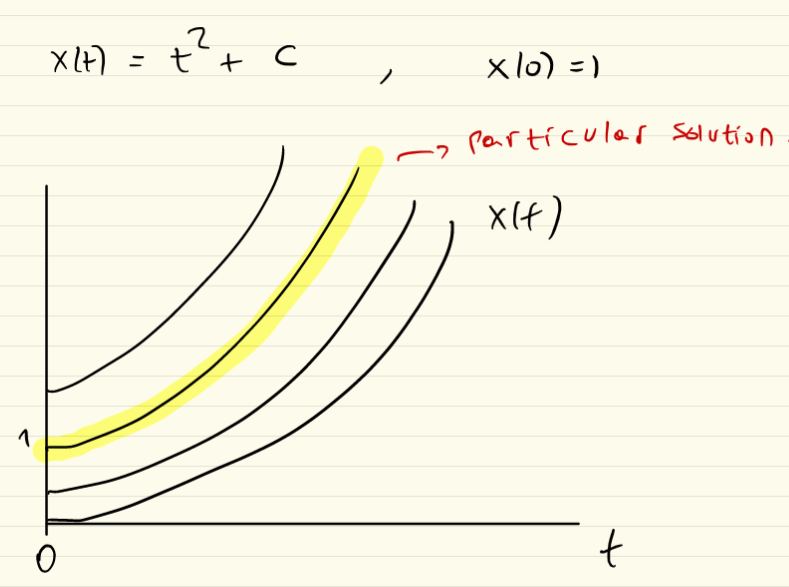
\includegraphics[width=4cm, height=3cm]{pic5}
            \end{center}
        \end{itemize}
    \end{itemize}
    \item  \underline{Finite-Difference Methods for Solution}: here we approximate derivates using finite-differences to approximate the solution to the ODE. This involves finding $\dot{x}(t) = F(t,x(t))$, $x(t_{a}) = x_{a}$, and $t \in [t_{a}, t_{b}]$. There are a wide range of methods depending on how the derivatives are approximated
    \begin{itemize}
        \item  \underline{Euler's Method}: given the equation implied by the ODE
        \begin{itemize}
            \item  \underline{Step 1}: specify a grid for t, i.e. $t_{0} = t_{a} < t_{1} < t_{2} < \dots < t_{N} = t_{b}$
            \item  \underline{Step 2}: we can approximate the ODE using the difference equation $$\frac{x(t_{i+1}) - x(t_{i})}{t_{i+1}-t_{i}} = F(t_{i},x(t_{i}))$$ iterating over $i = 0, \dots, N-1$, where $x(t_{0})=x_{a}$ is fixed by the initial condition
                \begin{itemize}
                    \item  \underline{Note}: the difference equation is obtained by rearranging the equation in step 1, we know all elements on the RHS of the difference equation which provides us with an explicit solution for $x(t_{1})$
                \end{itemize}
        \end{itemize}
        \item  \underline{Euler's Method Illustration}:
        \begin{itemize}
            \item  \underline{Step 1}: discretize $[t_{a}, t_{b}]$
            \item  \underline{Step 2}: iterate forward on $x(t_{i_1}) = x(t_{i}) + (t_{i+1} - t_{1})F(t_{i}, x(t_{i})) \ \ \ \forall i$
            \begin{itemize}
                \item \underline{i=0}: $x(t_{1}) = x(t_{0}) + (t_{1} - t_{0})F(t_{0}, x(t_{0}))$
                \item  \underline{i=1}: $\dots$ (etc)
            \end{itemize}
        \end{itemize}
        \item  \underline{Euler's Method Numerical vs Analytical Solution Equivalency}: $\dot{x}(t) = 2t, \ \ x(0)=1, \ \ t \in [0, 1000]$
            \newline
            \begin{center}
            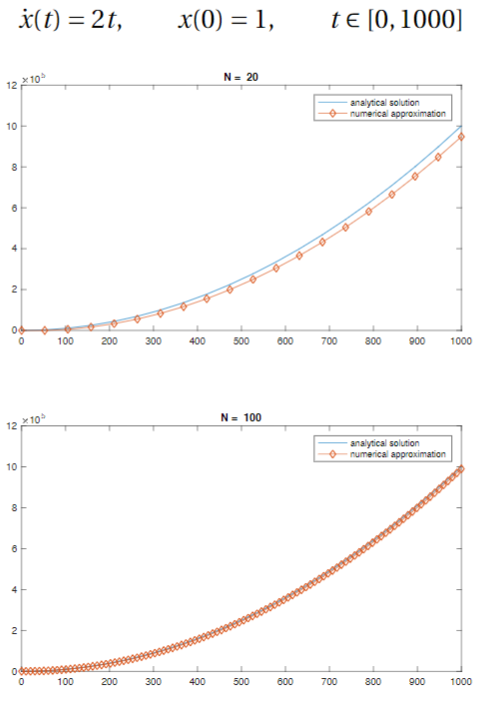
\includegraphics[width=5cm, height=3cm]{pic6}
            \end{center}
    \end{itemize}
    \item \underline{ODE Systems}: consider the system of two equations in two unknowns
    \begin{gather*}\dot{x}(t) = f(t, x(t), y(t)) \\ \dot{y}(t) = g(t, x(t), y(t)) \end{gather*} where $t \in [t_{a}, t_{b}]$. The general solution typically depends on two arbitrary constants,  say A and B, and can be written as \begin{gather*} x(t) = \phi_{1} (t; A, B) \\ y(t) = \phi_{2} (t; A,B) \end{gather*} Here the two arbitrary constants  A and B can be pinned down via two conditions on the solution which can causes two types of problems to emerge. In other words, the function must be solved such that either or both the initial and boundary conditions hold. Note that, like single-equation ODEs, exact solutions ODE systems can only be obtained under special cases
    \begin{itemize}
        \item \underline{Initial Value Problem(IVP)}: where you have conditions on the initial time ($a$) values - here $x(t_{a}) = x_{a}$, $y(t_{a}) = y_{a}$ can be solved numerically by applying Euler's Methods
        \begin{itemize}
            \item \underline{Step 1}: discretize the domain
            \item  \underline{Step 2}: iterate forward starting from $x(t_{a}) = x_{a}$ and $y(t_{a}) = y_{a}$
        \end{itemize}
        \item  \underline{Boundary Value Problem (BVP)}: where you have a condition on the value at a time period ($b$) that different from the initial time value ($a$). Here $x(t_{a}) = x_{a}$ and $y(t_{b}) = y_{b}$, which can be solved by applying a shooting algorithm
        \begin{itemize}
            \item \underline{Step 1}: make an initial guess for $y(t_{a})$ called $y_{a}^{G}$
            \item \underline{Step 2}: solve the ODE system by applying Euler's method given $x(t_{a}|y_{a}) = x_{a}$ and $y(t_{a}) = y_{a}^{G}$
            \item \underline{Step 3}: if $y(t_{b})$ is 'close enough' to $y_{b}$ then stop, else update $y_{a}^{G}$ and go back to step 2
            \newline
            \begin{center}
            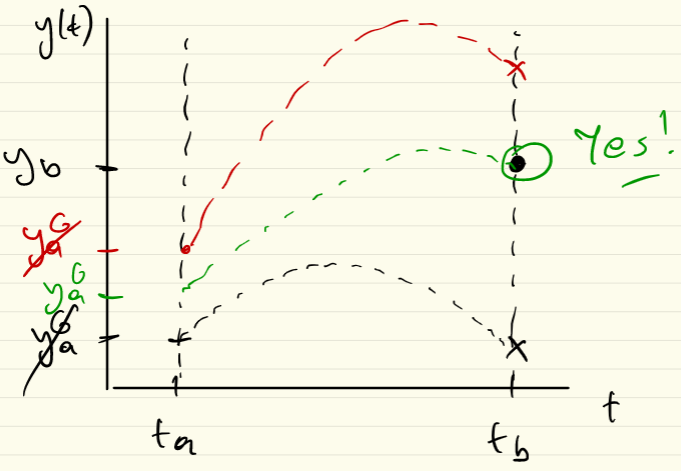
\includegraphics[width=4cm, height=3cm]{pic8}
            \end{center}
            \begin{itemize}
                \item  \underline{Note}: the solution must cause the value of $x(t_{a})$ to equal the a-priori $x(a)$ at time $t_{a}$ and the value of $y(t_{b})$ to equal the a-priori $y(b)$ at time $t_{b}$
            \end{itemize}
        \end{itemize}
    \end{itemize}
    \item \underline{Higher-Order ODEs}: techniques for solving ODE systems also apply to analysing higher-order Equations. Here we can express the second order ODE equation as a first order ODE system
    \begin{itemize}
        \item \underline{Example}: consider the second-order ODE \begin{gather*} \ddot{x}(t) = f(t, \dot(t), x(t)) \end{gather*} where $\ddot{x}(t) \equiv \partial^{2}x(t) / \partial t^{2}$.
        Define the new variables $y = \dot{x}$ and you are left with the two-equation ODE system
        \begin{gather*} \dot{y} (t) = f(t, y(t), x(t)) \\ \dot{x}(t) = y(t) \end{gather*}
    \end{itemize}
\end{itemize}
\vspace{2.5mm}
\par \underline{\bf{The Maximum Principle}}: the typical continuous time optimization problem is
\begin{gather*} \max_{x(t), y(t)} \ \int_{0}^{t_{1}} f (t,x(t), y(t)) \ \ \ dt \end{gather*}
subject to
\begin{gather*} \dot{x}(t) = g\big(t, x(t), y(t)\big), \ \ \ x(t) \in \mathcal{X} \ \forall t, \ \ \ y(t) \in \mathcal{Y} \ \forall t, \ \ \ x(0) = x_{0} \end{gather*}
There are two main issues with conventional solution methods to this problem; (1) we are choosing over infinitely dimensional objects such as the function $x: [0, t_{1}] \rightarrow \mathcal{X}$, (2) the constaints include a differential equation rather than a set of equalities/inequalities. In order to overcome these issues and find a solution, we apply the maximum principle theorem
\begin{itemize}
    \item \underline{Notation and Assumptions}: $x$ is the state variable, $y$ is the control variable, $\mathcal{X} \subset \mathbb{R}$  and $\mathcal{Y} \subset \mathbb{R}$ are nonempty and convex, $f$ and $g$ are continuously differentiable in their arguments, we define a Hamiltonian, and for simplicity we assume $t_{1} < \infty$
    \begin{itemize}
        \item  \underline{Hamiltonian}: we define the hamiltonian $$H(t,x(t),y(t),\mu(t)) \equiv f(t,x(t),y(t)) + \mu(t)g(t,x(t),y(t))$$ where $\mu(t)$ is a continuously differentiable function called the costate variable
    \end{itemize}
    \item  \underline{Maximum Principle Theorem}: suppose that the aforementioned continuous time problem has an interior continuous solution $(\widehat{x}(t), \widehat{y}(t))$. Then there exists a continuously differentiable function $\mu(t)$ such that
    \begin{gather*} H_{y}(t,\widehat{x}(t), \widehat{y}(t), \mu(t)) = 0 \ \ \forall t \in [0, t_{1}] \\ \dot{\mu}(t) = -H_{x}(t, \widehat{x}(t), \widehat{y}(t), \mu(t)) \ \ \forall t \in [0, t_{1}] \\ \mu(t_{1}) = 0
    \end{gather*}
    These operate as the necessary conditions for the Hamiltonian
    \begin{itemize}
        \item \underline{ODE Usage}: by $H_{y}(t,\widehat{x}(t), \widehat{y}(t), \mu(t)) = 0$ we can solve for $y$ as a function of $x$ thereby writting $y = Y(t, x \mu)$. Plugging $y = Y(t, x \mu)$ into $\dot{\mu}(t) = -H_{x}(t, \widehat{x}(t), \widehat{y}(t), \mu(t))$ and $ \dot{x}(t) = g\big(t, x(t), y(t)\big)$ and combining the law of motion we are left with
        \begin{gather*} \dot{x} = g\big(t, x, Y(t,x,\mu)\big) \\ \dot{\mu} = -H_{x}\big(t,x,Y(t,x,\mu),\mu \big) \\ x(0) = x_{0}, \ \ \ \mu(t_{1}) = 0 \end{gather*}
        which is an ODE system in $x$ and $\mu$ that can be solved numerically by applying the shooting algorithm
        \item \underline{Sufficient Condition Requirements}: the maximum principle only provides necessary conditions for an optimum, sufficient conditions for a maximum rely on concavity properties of the objective and on convexity of the feasible set
        \item \underline{Technique Generalization}: the techniques generalize to multidimensional problems (where $x$ and $y$ are vectors), infinite horizon problems (ie $t_{1} = \infty$), and to including terminal conditions on the final state (e.g. $x(t_{1}) = x_{1}$)
        \item \underline{Index}: the variable t may represent time or any other index
    \end{itemize}
\end{itemize}
\vspace{2.5mm}
\par \underline{\bf{Heuristic Proof of The Maximum Principle}}: to solve problem $(x)$ it would be natural to start trying "some sort" of lagrangian optimization such as constructing the function \begin{gather*} \mathcal{L} = \int_{0}^{t_{1}} \left\{F(t, x(t), y(t)) + \mu(t)[g(t,x(t), y(t)) - \dot{x}(t)] \right\} \end{gather*} where $\mu(t)$ is a continuously differentiable function from the hamiltonian. Supposing that $(\widehat{x}(t), \widehat{y}(t))$ is an interior solution to the lagrange problem, then $(\widehat{x}, \widehat{y})$ should maximize $\mathcal{L}$.
\begin{itemize}
    \item \underline{Lemma}: the function $\mathcal{L}$ can be written as \begin{gather*} \mathcal{L} = \int_{0}^{t_{1}} \left\{ f(t,x(t),y(t)) + \mu(t)g(t,x(t),y(t)) + \dot{\mu}(t)x(t) \right\} \ \ dt - \mu(t_{1})x(t_{1}) + \mu(0) x(0) \end{gather*}
    \begin{itemize}
        \item \underline{Proof}: note that
        \begin{gather*} \int_{0}^{t_{1}} \tfrac{\partial (\mu(t)x(t))}{\partial t} \ \ dt = \int_{0}^{t_{1}} \dot{\mu}(t)x(t) \ \ dt + \int_{0}^{t_{1}} \mu(t)\dot{x}(t) \ \ dt
        \end{gather*}
        If we integrate both sides over $[0, t_{1}]$ then we have
        \begin{gather*}
            \mu(t_{1})x(t_{1}) - \mu(0)x(0) = \int_{0}^{t_{1}} \dot{\mu}(t) x(t) \ \ dt + \int_{0}^{t_{1}} \mu(t)\dot{x}(t) \ \ dt
        \end{gather*}
        This can be rearranged as
        \begin{gather*} \mu(t)\dot{x}(t) \ \ dt = \mu(t_{1})x(t_{1}) - \mu(0)x(0) - \int_{0}^{t_{1}} \dot{\mu}(t)x(t) \ \ dt
        \end{gather*}
        Plugging this into our lagrangian yields the above lemma
    \end{itemize}
    \item \underline{Proof of Function Features}: consider a variation/perturbation around the optimal path $(\widehat{x}(t), \widehat{y}(t))$. Specifically, take an arbitrary function $P_{y}(t)$, let $\varepsilon \in \mathbb{R}$, and define $y(t, \varepsilon) = \widehat{y}(t) + \varepsilon P_{y}(t)$. Here$y(t, \varepsilon)$ is the solution plus a deviation from the solution ($\widehat{y}(t) + \varepsilon P_{y}(t)$) Graphically
    \newline
    \begin{center}
    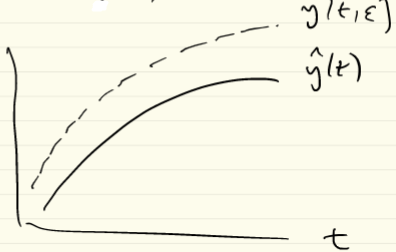
\includegraphics[width=4cm, height=3cm]{pic9}
    \end{center}
    Similarly, let $x(t, \varepsilon) = \widehat{x}(t) + \varepsilon P_{x}(t)$ where $P_{x}(t)$ denotes the corresponding perturbation to $\widehat{x}(t)$ when $\widehat{y}(t)$ is varied according to $P_{y}(t)$. Note that the sum of the perturbations is the variation around the optimum. Define the 'perturbed' lagrangian function as
    \begin{gather*}
    \mathcal{L}(\varepsilon) = \int_{0}^{t_{1}} \left\{ f(t,x(t,\varepsilon),y(t,\varepsilon)) + \mu(t)g(t,x(t,\varepsilon),y(t,\varepsilon)) + \dot{\mu}(t) x(t,\varepsilon) \right\} \ \ dt - \mu(t_{1})x(t_{1}, \varepsilon)+\mu(0)x_{0}
    \end{gather*}
    Recall that $\mathcal{L}$ is maximized at $\widehat{x},\widehat{y}$, where the marginal gain from increasing $\varepsilon$ (ie the perturbation) is 0, and therefore we must have
    \begin{gather*}
    \tfrac{\partial \mathcal{L}(\varepsilon)}{\partial \varepsilon} | (\varepsilon, x, y) = (0, \widehat{x}, \widehat{y}) = 0
    \end{gather*}
    Using the definitions of $x(t,\varepsilon)$, $y(t,\varepsilon)$, and $\mathcal{L}$ the above equation can be expressed as:
    \begin{align*}
     0 = &\int_{0}^{t_{1}} \Big\{ \overbrace{f_{x}(t,\widehat{x}(t),\widehat{y}(t)) + \mu(t)g_{x}(t,\widehat{x}(t),\widehat{y}(t))}^{ \begingroup\color{magenta} H_{x}(t,\widehat{x}(t), \widehat{y}(t), \mu(t)) \endgroup} + \dot{\mu}(t) \Big\} P_{x}(t) \ \ dt \\ &+ \int_{0}^{t_{1}} \underbrace{\Big\{f_{y}(t,\widehat{x}(t), \widehat{y}(t)) + \mu(t)g_{y}(t,\widehat{x}(t), \widehat{y}(t)) \Big\} }_{\begingroup\color{magenta}H_{y}(\cdot)\endgroup} P_{y}(t) \ \ dt - \mu(t_{1})P_{x}(t_{1})
    \end{align*}
    \begin{itemize}
        \item  \underline{Note}: this expression can only hold for all feasible perturbation paths $(P_{x}, P_{y})$ if each integrand vanishes and $\mu(t_{1}) = 0$ such that $P_{y}(t)$ and $P_{x}(t)$ equal 0, which are the conditions of the maximum principle
    \end{itemize}
\end{itemize}
\vspace{2.5mm}
\par \underline{Problem Example 1}: consider the optimal consumption problem of an agent living between two dates, 0 and 1. Time is continuous and the individual has an instantaneous utility function $\ln(c)$ over consumption $c$ and discount future payoffs exponentially at rate $p > 0$. \\ Let $a(t) \geq 0$ be the level of assets of the agent at time $t$. Assume that the individual starts with assets $a(0) = \overline{a} > 0$ and has to end up with zero assets at the end of her planning horizon such that $a(1) = 0$. At every point in time, the individual obtains income from two sources: interest $r > 0$ on asset holdings and labour earnings $w > 0$. \\ The lifetime utility maximization problem can be written as:
\begin{gather*}
    \max_{c(t) \geq 0, a(t) \geq 0} \ \int_{0}^{1} \exp (- \rho t) \ln (c(t)) dt \\
    \text{subject to} \\
    \cdot{a}(t) = r a(t) + w - c(t) \\
    a(0) = \overline{a}, \ \ a(1) = 0
\end{gather*}
\begin{itemize}
    \item  \underline{Question 1}: write up the Hamiltonian of the consumer's problem. In doing so, let $\mu(t)$ be the costate variable
    \begin{itemize}
        \item  \underline{Solution}: $H = \exp (-\rho t) \ln (c(t)) + \mu(t) (ra(t) + w - c(t))$
    \end{itemize}
    \item  \underline{Question 2}: show that the optimal solution satisfies the following system of differential equation in $\mu(t)$ and $a(t)$:
    \begin{gather*}
        \cdot{a}(t) = ra(t) + w - \frac{\exp(-\rho t)}{\mu(t)} \\
        \cdot{\mu}(t) = - \mu(t) \rho
    \end{gather*}
    with $a(0) = \overline{a}$ and $a(1) = 0$. (Hint: given the terminal condition $a(1) = 0$, this problem does not feature the condition $\mu(1) = 0$)
    \begin{itemize}
        \item  \underline{Solution}:
        \begin{arrange*}
            \frac{\partial H}{\partial c} = 0 \Rightarrow \frac{\exp(-\rho t)}{c(t)} - \mu &= 0 \\
            \therefore c(t) = \frac{\exp (-\rho t)}{\mu (t)}
        \end{arrange*}
        \begin{gather*}
            \frac{\partial H}{\partial a} = - \cdot{\mu}(t) \Rightarrow \cdot{\mu}(t) = -\mu(t)\rho \tag{*} \\
        \end{gather*}
        \begin{gather*}
            \mu(t) = 0
        \end{gather*}
        Plugging $c(t) = \frac{\exp (-\rho t)}{\mu (t)}$ into our constraint we have:
        \begin{gather*}
            \cdot{a}(t) = ra(t) + w - \frac{\exp(\rho t)}{\mu (t)}
        \end{gather*}
    \end{itemize}
    \item  \underline{Question 3}: show that $\mu(t) = \mu(0) \exp (-\rho t)$ so that optimal assets evolve according to $\cdot{a}(t) = ra(t) + w - \tfrac{\exp ((r-\rhi)t)}{\mu(0)}$
    \begin{itemize}
        \item  \underline{Solution}: by equation (*) we have $\tfrac{\cdot{\mu}(t)}{\mu(t)} = \rho$. Note that $\cdot{\mu}(t) = \partial \mu(t)$ and therefore:
        \begin{gather*}
            \frac{\partial \mu(t)}{\mu(t)} = -\rho \tag{**}
        \end{gather*}
        Multiplying the equation (**) by the integrand $\in [0, t]$ and taking the derivative with respect to $t$ on both sides we have:
        \begin{gather*}
            up to here
        \end{gather*}
    \end{itemize}
    \item  \underline{Question 4}: how does the difference between the subjective discount rate $\rho$ and the interest rate $r$ affect the optimal consumption path $c(t)$
    \begin{itemize}
        \item  \underline{Solution}:
    \end{itemize}
\end{itemize}

\newpage

\section{Enforcement Frictions I - One-Sided}

\vspace{2.5mm}
\par \underline{Overview}: the analysis of contractual arrangements and enforcement frictions aims to rectify conflicts of interest that arise from violations of two assumptions - (1) both parties were perfectly committed to the rules of the exchange, (2) both parties in the exchange shared the same information. Dropping either of these assumptions creates conflicts of interest
\begin{itemize}
    \item  \underline{Assumption 1 Violation}: here an agent who is not committed to the rules of the exchange would deviate from such rules when she finds it more convenient
    \item  \underline{Assumption 2 Violation}: here an agent who possesses private information would manipulate such information to her advantage
\end{itemize}
\vspace{2.5mm}
\par \underline{Contract Theory}: the study of the economic aspects of contract design where a contract is a set of rules that facilitates cooperation among individuals with conflicting objectives. The goal of contract theory is twofold with the normative goal of how to draw up better contracts and the positive goal of analysing why real life contracts have various forms and designs. We can arbitrarily classify contract theory models by two classifications - (1) according to the type of private information, (2) according to the duration of the contractual relationship
\begin{itemize}
    \item \underline{Type of Private Information}: here we assume that the uninformed party designs the contract and address two types of information issues (adverse selection and moral hazard)
    \begin{itemize}
        \item  \underline{Adverse Selection}: asymmetric information about the characteristics of the informed party (e.g. life insurance where the insured's state of health is unknown by the insurer)
        \item  \underline{Moral Hazard}: asymmetric information about the actions of the informed party (e.g. CEO compensation where the CEO's actions are imperfectly observed by the Board of Directors)
    \end{itemize}
    \item  \underline{Duration of Contractual Relationship}: here we address two types of contract periods (static and dynamic)
    \begin{itemize}
        \item  \underline{Static Contracts}: relationship lasts for one period
        \item  \underline{Dynamic Contracts}: relationship lasts for more than one period (gives rise to enforcement/commitment issues)
    \end{itemize}
\end{itemize}
\vspace{2.5mm}
\par \underline{Principal-Agent Paradigm}: since contracts involve two parties we need to address how the parties bargain over  the terms of the exchange. We bypass the difficulties inherent to the bargaining process by allocating all bargaining power to one of the parties (the Principal) who will offer a take-it or leave-it contract to the Agent. The Principal-Agent Paradigm is the norm in contract theory
\begin{itemize}
    \item \underline{w.l.o.g}: the set of Pareto optimal contracts can be characterised by maximizing the utility of one agent subject to a given level of utility of the other agent. This outcome is a result of the Principal-Agent analogy
\end{itemize}
\vspace{2.5mm}
\par \underline{Enforcement Frictions}: occur when agents are free to walk away from the contract at any time, note that for most models of enforcement frictions we assume that all information is public
\begin{itemize}
    \item  \underline{One-Sided Limited Commitment}: occurs when the principal is committed but the agent is not
    \begin{itemize}
        \item \underline{Applications}: long term labour contracts (principal is the firm and agent is the worker), international lending (principal is the lending country and agent is the borrowing country), firm dynamics (principal is the bank, agent is the entrepreneur seeking to finance a project)
    \end{itemize}
\end{itemize}
\vspace{2.5mm}
\par \underline{Basic Model}: the economy lasts for $T = \infty$ periods and consists of a village with a large number of households. Household preferences are
\begin{gather*}
    U = \mathbb{E}_{0} \sum_{t = 0}^{\infty} \beta^{t} u(c_{t})
\end{gather*}
where $\beta \in (0, 1)$ and $u$ is concave and has the usual properties. \\ \\ Each HH receives a stochastic endowment stream $\left\{y_{t}\right\}_{t=0}^{\infty}$ where $y_{t} \in \left\{ \overline{y}_{1}, \overline{y}_{2}, \dots, \overline{y}_{S} \right\}$ and $\overline{y}_{s+1} > \overline{y}_{s}$. Note that for each $t \geq 0$, $y_{t}$ is independently and identically distributed according to the discrete probability distribution $\Pr(y_{t} = \overline{y}_{s}) = \pi_{s}$ where $s$ is the set from which HHs draw endowments from. At time $t\geq 1$ the household has received a history of endowments $h_{t} = (y_{t}, y_{t-1}, \dots, y_{0})$
\begin{itemize}
    \item \underline{Assumptions}: the endowment processes are iid both across time and across households, overline represents the realizations of the endowments, due to concavity HHs value insurance against endowment realizations, $y_{t}$ is non-storable and therefore self-insruance is precluded
    \item \underline{No Contractual Issue Solution}: if there were a competitive equilibrium with complete markets, at $t=0$ HHs would trade history and date contigent claims before the realization of endowments. Since all HHs are ex ante identical, each HH would end up consuming the per capita endowment in every period and their its lifetime utility would be
    \begin{gather*}
        v_{pool} = \sum_{t=0}^{\infty} \beta^{t} u \Big( \sum_{s=1}^{S} \Pi_{s} \overline{y}_{s} \Big) = \frac{1}{1-\beta} u \Big( \sum_{s=1}^{S} \Pi_{s}\overline{y}_{s} \Big)
    \end{gather*}
    HHs would thus insure away all of the risk associated with their individual endowment process. However, due to limited commitment and other contractual issues, this allocation is unattainable
\end{itemize}
\vspace{2.5mm}
\par \underline{One-Sided Limited Commitment Contract Issue}: in this case, the HH can only trade with the moneylender and can walk away from the contract. If the HH walks away then the HH consumers their endowment and lives in autarky evermore (i.e. the HH cannot return from autarky). Note that only the HH can break the contract, while the moneylender is fully committed to keeping their promise. Therefore, HHs must be induced not to walk away from the contract via structuring the contract in such a way that it is "self-enforcing" in that HHs prefer to conform to it. \\ \\
This involves a contract between the moneylender and the HH as a sequence of history dependent functions $\left\{c_{t}\right\}_{t=0}^{\infty}$ with $c_{t} = f_{t} (y^{t})$. The contract specifies that in each period the HH contributes her endowment realization $y_{t}$ to the moneylender in exchange for consumption $c_{t}$. \\ \\
From this arrangement, the moneylender earns an ex ante expected present value
\begin{gather*}
    P = \mathbb{E}_{0} \sum_{t=0}^{\infty} \beta^{t} (y_{t} - c_{t})
\end{gather*}
where $(y_{t} - c_{t})$ is the net transfer from HH at time t. The moneylender seeks to maximize the expected present value of profits from making contracts. \\ \\
Given the HHs preferences in the basic model, the contract assigns the HH an expected present value of
\begin{gather*}
    v = \mathbb{E} \sum_{t=0}^{\infty} \beta^{t} u(c_{t})
\end{gather*}
If the HH walks away from the contract, the ex ante value associated with consuming the endowment stream in autarky is
\begin{gather*}
    v_{aut} = \mathbb{E}_{0} \sum_{t=0}^{\infty} \beta^{t} u(y_{t}) = \frac{1}{1-\beta} \sum_{s=1}^{S} \Pi_{s} u(\overline{y}_{s})
\end{gather*}
where the continuation utility under autarky is the weighted sum of the possible realizations from the endowment (which due to iid we can remove the dependency of $y$ on time). Note that at time $t$ the HH can guarantee itself a present value of utility of $u(y_{t}) + \beta v_{aut}$ by consuming its own endowment and therefore the moneylender's contract must offer the HH at least this utility at every possible history and every date (this forms the basis of the participation constraint). \\ \\
Here the optimal contract can be analysed using recursive tools, this relies on the inclusion of a participation constraint and promise constraint to entice the HH to stay in the contract
\begin{itemize}
    \item  \underline{Assumptions}: information is symmetric and therefore the moneylender can observe $y_{t}$, the HHs cannot borrow or lend with one another and can only trade with the moneylender, the money lender is risk-neutral and can borrow or lend at the risk free rate $R = \beta^{-1}$, only the money lender has access to the risk-free loan market outside the village, $R$ is exogeneous (i.e. this is a partial equilibrium model)
    \item  \underline{Notation}: our variables include
    \begin{align*}
    &\beta \in (0,1): \ \text{the discount factor} \\
    &c_{t}:\ \text{the consumption that the moneylender gives to the HH in exchange for the endowment $y_{t}$ under the contract} \\
    &y_{t}:\ \text{the endowment that the HH receives in time period $t$} \\
    &y^{t}:\ \text{refers to the endowment history up until time t (i.e. the sum of prior endowments)} \\
    &\overline{y_{s}}: \ \text{the observed endowment that is realized at time $t$} \\
    &W_{t}: \ \text{the sum of the money lender's net gains from each previous period's contract up until time t} \\
    &w_{s}: \ \text{refers to the moneylender's utility transfer to the HH the contract given a particular future state $s$ from time $t$ onwards} \\
    &\text{$\sum_{s=1}^{S}$} \Pi_{s} w_{s}: \ \text{the money lender's expected utility transfer to the HH from time $t \rightarrow \infty$} \\
    &v_{aut}: \ \text{the sum of future endowments (as utility) that the HH receives if living in autarky} \\
    &v_{t}: \ \text{the discounted sum of future gains (as utility) that the HH receives under the contract from time $t$ onwards} \\
    &s: \ \text{refers to the different possible states at at a given time period}
\end{align*}
    Here unspecified $t$ refers to present time.
    \item  \underline{HH "Forward-Looking" State Variable}: note that for the HH, under the contract, the state variable is the promised expected discounted future value (i.e. the sum of all future earnings from the contract). In otherwords, the HH's state variable $v_{t}$ is a "forward-looking" variable where  $v_{t} = \mathbb{E}_{0} \sum_{j=0}^{\infty} \beta^{j} u(c_{t+j})$. This "forward-looking" variable summarizes a stream of future utilities
    \item \underline{Moneylender "Backward-Looking" State Variable}: note that for the moneylender, under the contract, the state variable is the total net gain $(y- c)$ at time $t$. In otherwords, the moneylender's state variable $W_{t}$ is a "backward-looking" variable where $W_{t} = \sum_{t=0}^{t=T} (y_{t} - c_{t})$ (i.e. $W_{t}$ encodes all history dependence in the contract)
    \begin{itemize}
        \item \underline{Logic}: to see how this works, consider the following way of representing a contract $\left\{ f_{t} \right\}$ in terms of a state variable $x_{t}$:
        \begin{align*}
            c_{t} &= g(x_{t}) \\
            x_{t+1} &= \mu (x_{t}, y_{t})
        \end{align*}
        Here $g$ and $\mu$ are time-invariant functions. Notice that by iterating the $\mu(\cdot)$ function $t$ times starting from $(x_{0}, y_{0})$, one obtains
        \begin{gather*}
            x_{t} = m_{t}(x_{0}; y_{t-1}, \dots, y_{0}), \ \ \ t \geq 1
        \end{gather*}
        This allows one to summarize large dimensional shocks and rewards into a single variable and thus $x_{t}$ summarizes histories of endowments
    \end{itemize}
    \item \underline{Participation Contraint}: since autarky is the outside option of the agents, the optimal contract must satisfy the participation constaints where the value of the contract is worth more than the value of autarky and is therefore "self-enforcing" (otherwise the HH will default). Since the money lender arrives at period $y$ before $y_{t}$ is realized and having previously made promised value $v_{t}$ our participation constraint is:
    \begin{gather*}
        u(\overbrace{f_{t}(y^{t})}^{\begingroup\color{magenta} c_{t} \endgroup}) + \underbrace{\beta \mathbb{E}_{t} \sum_{j=1}^{\infty} \beta^{j-1} u(\overbrace{f_{t+j}(y^{t+j})}^{\begingroup\color{magenta} c_{t+j} \endgroup})}_{\begingroup\color{magenta} w_{t}(y^{t}): \ \text{continuation utility at t} \endgroup} \geq u(y_{t}) + \beta v_{aut}
    \end{gather*}
    for all $t, y^{t}$ \\
    We can rewrite our participation constraints as
    \begin{gather*}
        u(f_{t}(y^{t})) + \beta \begingroup\color{cyan} w_{s}(y^{t}) \endgroup \geq u(y_{t}) + \beta v_{aut}
    \end{gather*}
    for all $t, y^{t}$ where
    \begin{gather*}
        \begingroup\color{cyan} w_{s}(y^{t}) \endgroup \equiv \mathbb{E}_{t} \sum_{j=1}^{\infty} \beta^{j-1} u(f_{t+j} (y^{t+j}))
    \end{gather*}
    is the continuation utility of the agent at time $t$, given endowment history $y^{t}$
    \item  \underline{Promise Keeping Constraint}: the Promise Keeping Constraint states that the amount the HH gets in expectation must be greater than $v$, in other words the moneylender must be able to fulfil the contract such that
    \begin{gather*}
        \sum_{s=1}^{S} \Pi_{s} [u(c_{s}) + \beta w_{s}] \geq v
    \end{gather*}
    \item  \underline{Moneylender Problem}: each period the money lender chooses how much to give to the HH and how much that they will promise to transfer in the future (which is encoded in $w_{s}$) in order to make the contract "self-enforcing". Here the moneylender chooses $c_{s}$ and a promised value starting in the next time period $v$. Therefore, the the money lender solves
    \begin{gather*}
        P(v) = \max_{\left\{ c_{s}, w_{s} \right\} } \sum_{s=1}^{S} \Pi_{s} [\overline{y}_{s} - c_{s} + \beta P(w_{s})]
    \end{gather*}
    subject to
    \begin{align*}
        \sum_{s=1}^{S} \Pi_{s} [u(c_{s}) + \beta w_{s}] \geq v & \rightarrow \ \text{Promise Keeping Constraint} \\
        u(c_{s}) + \beta w_{s} \geq u(\overline{y}_{s}) + \beta v_{aut}, \ \ s = 1, \dots, S & \rightarrow \ \text{Participation Constraint}
    \end{align*}
    Here $w_{s} \in [v_{aut}, \overline{v}]$ where $\overline{v}$ is a large number. $w_{s}$ is the \textit{future} (i.e. next period) realized transfer under the contract established at time $t$ given state possible $s$, given that $y = \overline{y}_{s}$ this period. $w_{s}$ therefore represents the promised value which the HH will enter next period). We treat promised utility $v$ as a state variable for the HH. Note that $P$ must be a decreasing function of $v$ because the higher the consumption stream of the villager, the lower must be the profits of the moneylender
    \begin{itemize}
        \item  \underline{Characterisation}: it can be shown that the constraint set is convex and that the value function $P(v)$ is stictly concave (as well as differentiable). Given this we have the following lemmas that essentially state that agents have incentives to walk away when income realisations are large enough - wherein the participation constraint will bind for a $\overline{y}_{s}$ that is significantly high.

        \begin{itemize}
            \item \underline{Lemma 1}: for each $v$, there exists a threshold $\overline{y}(v)$ such that the PC binds binds if and only if $\overline{y}_{s} \geq \overline{y}(v)$
            \begin{itemize}
                \item  \underline{Logic}: in other words, for every possible "discounted sum of future gains", there exists a theshold endowment level such that the PC will bind if the actual endowment level is greater or equal to the figurative endowment level. This makes sense, since if the HH receives a particularly high endowment this period then the moneylender will offer distribute $y_{t}$ with a lower proportion of $u(c_{t})$ (though still a higher level of $u(c_{t})$) and a higher proportion $c_{t+j}$ to make the contract "self-enforcing"
            \end{itemize}
            \item  \underline{Lemma 2}: the threshold $\overline{y}(v)$ is increasing in v
            \begin{itemize}
                \item  \underline{Logic}: this makes sense since a higher $v$ occurs when $c_{s+j}$ increases. $c_{t+j}$ increases when $\overline{y}(v)$ is reached, with the moneylender offering a lower proportion (relative to $y_{s}$) of $u(c_{t})$ as part of the contract (though $u(c_{t})$ will still be higher than when receiving $y_{1} < y_{s}$)
            \end{itemize}
            \item  \underline{Proof}: we write the lagrangian as
            \begin{gather*}
                \mathcal{L} = \sum_{s=1}^{S} \Pi_{s} [\overline{y}_{s} - c_{s} + \beta P(w_{s})] \\ + \varepsilon \left\{ \sum_{s=1}^{S} \Pi_{s} [u(c_{s}) + \beta w_{s} - v \right\} \\ +  \sum_{s=1}^{S} \eta_{s} \left\{ u(c_{s}) + \beta w_{s} - u(\overline{y}_{s}) - \beta v_{aut} \right\}
            \end{gather*}
            where $\varepsilon$ and $\eta$ are the lagrangian multipliers on the Promise Keeping Constraint and Participation Contraint respectively. Taking first order conditions and applying the envelope theorem yields the following:
            \begin{align*}
                \frac{\partial \mathcal{L}}{\partial C_{s}} = 0 &\rightarrow -\Pi_{s} + \varepsilon \Pi_{s} u^{'}(C_{s}) + \eta_{s} u^{'} (C_{s}) = 0 \tag{1} \\
                \frac{\partial \mathcal{L}}{\partial w_{s}} = 0 &\rightarrow \eta_{s} + \varepsilon \Pi_{s} = - \Pi_{s}P^{'}(w_{s}) \tag{2} \\
                \text{Envelope Theorem}: \ \ &\rightarrow P'(v) = - \varepsilon < 0 \tag{3}
            \end{align*}
            Rearranging equations $(1)$ and $(2)$ for $\varepsilon \Pi_{s} + \eta_{s}$ and solving them simultaneously yields
            \begin{align*}
                u^{'}(C_{s}) = - P^{'}(w_{s})^{-1} \tag{4}
            \end{align*}
            It is clear to see that the LHS of this equation falls with $C_{s}$ due to concavity of $u(\cdot)$ and the RHS of this equation falls with $w_{s}$ due to concavity of $P(\cdot)$. This implies that $C_{s}$ and $w_{s}$ are positively related. In otherwords, as our lemma states, a higher $C_{s}$ results in a higher $w_{s}$
            \newline
            Combining $(3)$ and $(2)$ yields the law of motion for continuation Utility
            \begin{align*}
                P^{'}(w_{s}) = P^{'}(v) - \frac{\eta_{s}}{\Pi_{s}} \tag{5}
            \end{align*}
            \newline
            \underline{Lemma 1 Proof}
            \newline
            Take as given that $\overline{y}_{s}$ subject to PC is not binding (i.e. $\eta_{s} = 0$), therefore by $(5)$ we have
            \begin{gather*}
                P^{'}(w_{s}) = P^{'}(v) \Rightarrow w_{s} = v \ \ \text{by concavity}
            \end{gather*}
            Using this fact into $(4)$ we can write $c$ as a function of only $v$ and so have
            \begin{gather*}
                u^{'}(C_{s}) = -P^{'} (v)^{-1}
            \end{gather*}
            Which can be rewritten as $C_{s} = g_{1}(v), \ \ g_{1}^{'} > 0$. This allows us to rewrite the PC as
            \begin{gather*}
                u(C_{s}) + \beta w_{s} > u(\overline{y}_{S}) + \beta v_{aut} \\
                \Big\Downarrow \\
                u(g_{1}(v)) + \beta v > u(\overline{y}) + \beta v_{aut} \equiv \overline{y}(v) \\
                \Big\Downarrow \\
                \underbrace{u^{-1} (u(g_{1}(v)) _ \beta (v-v_{aut}))}_{\begingroup\color{cyan} \equiv \overline{y}(v) \endgroup} > \overline{y_{s}}
            \end{gather*}
            Thus, given the definition of $\overline{y}(v)$, the PC is not binding if and only if $\overline{y}_{s} < \overline{y}(v)$
            \newline
            \underline{Lemma 2 Proof}
            \newline
            Given the definition of $\overline{y}(v)$ from the proof for Lemma 1, this is straightforward
                \newline
                \begin{center}
                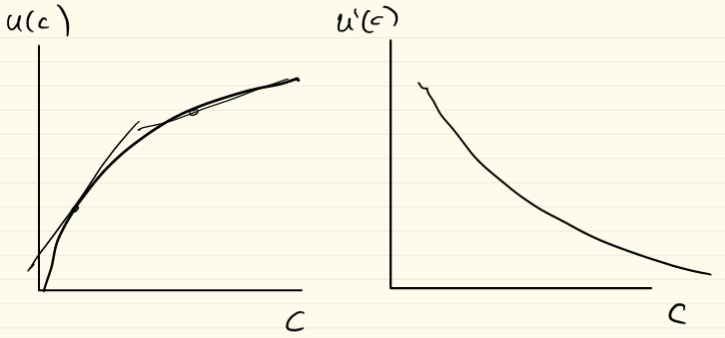
\includegraphics[width=4cm, height=3cm]{pic11}
                \end{center}
        \end{itemize}
    \end{itemize}
    \item \underline{Properties of PC Binding vs Not Binding}
    Suppose PC is not binding, then $w_{s} = v$ and $C_{s} = g_{1}(v)$ where $g_{1}^{'} > 0$. Therefore, if PC is not binding then $w_{s}$ and $C_{s}$ remain constant with consumption in state $s$ depending on promised utility $v$ but not on the endowment in state $s$ \\ \\
    Suppose PC is binding, then $w_{s} = l(\overline{y}_{s}) > v$ and $C_{s} = g_{2}(\overline{y}_{s}) \in (g_{1}(v), \overline{y}_{s})$ where $l^{'}, g_{2}^{'} \geq 0$. \\ \\ Therefore, if PC is binding then $w_{s}$ and $C_{s}$ must increase to induce the agent not to walk away from the contract - wherein $w_{s}$ and $c_{s}$ only depend on current income realisations (and not on the history of shocks given by $v$)
    \begin{itemize}
        \item \underline{Consumption under Optimal Contract}: graphically, given v, consumption under the optimal contract is
            \newline
            \begin{center}
            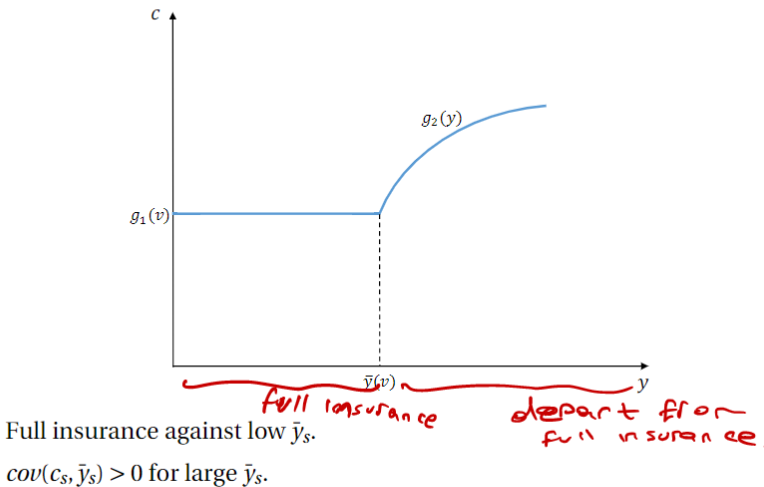
\includegraphics[width=8cm, height=6cm]{pic12}
            \end{center}
        \item \underline{Long Run Dynamics}: $c_{t}$ increases over time until $\overline{y}_{S}$ is realized.
            All agents eventually become fully insured (no fluctuations in consumptions) when their highest income realization $\overline{y}_{S}$ is realized and therefore $C$ eventually becomes constant.
            \newline
            \begin{center}
            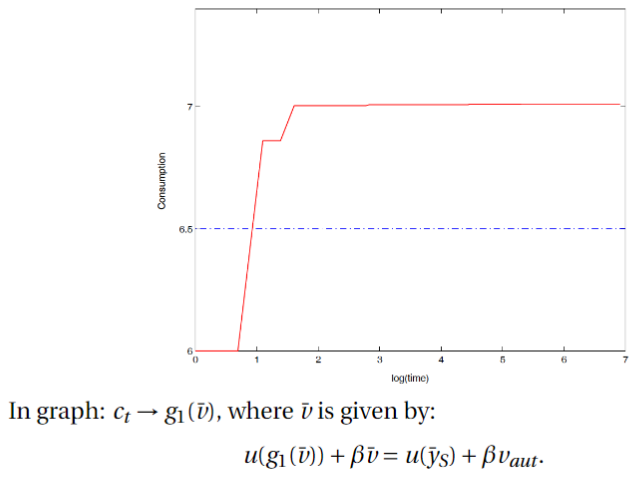
\includegraphics[width=8cm, height=6cm]{pic13}
            \end{center}
            With many HHs, all agents eventually get to consume $g_{1}(\overline{v})$: $\lim_{t \rightarrow \infty} \Pr(c_{t} = g_{1}(\overline{v})) = 1$. Overall, we have "fanning in" of the cross-sectional distribution of consumption and full risk sharing in the long run (ie t=500)
            \newline
            \begin{center}
            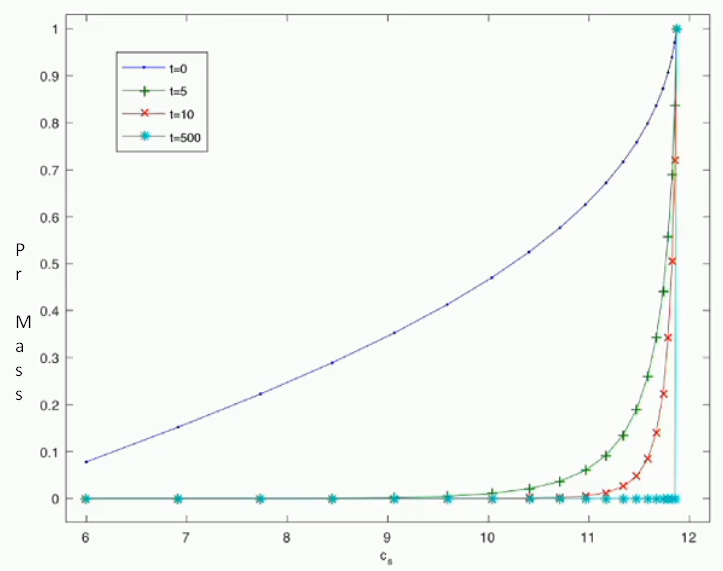
\includegraphics[width=8cm, height=6cm]{pic14}
            \end{center}
        \item  \underline{Not Binding Proof}: shown in the proof of the lemma
        \item  \underline{Binding Proof}: assume that PC is binding
        \begin{itemize}
            \item \underline{Step 1}: show that $w_{s}$ and $c_{s}$ are only functions of $\overline{y}_{s}$
            \newline
            By FOC $(4)$ we have $u^{1} (C_{s}) = -P^{'}(w_{s})^{-1}$ and given the fact that PC is binding we have $u(C_{s}) + \beta w_{s} = u(\overline{y}_{s}) + \beta v_{aut}$. Note that these two equations form a system of 2 equations in 2 unknowns ($C_{s}, w_{s}$). Since promised $v$ does not show up in this system we can write its solution as $w_{s} =l(\overline{y}_{s})$ and $C_{s} = g_{2}(\overline{y}_{s})$
            \item  \underline{Step 2}: show that $g_{2}^{'} > 0$ and $l^{'} > 0$
            \newline
            By $u(C_{s}) + \beta w_{s} = u(\overline{y}_{s}) + \beta v_{aut}$ we know that $[u(C_{s}) + \beta w_{s}]$ is non-decreasing in $\overline{y}_{s}$. Also, by $u^{1} (C_{s}) = -P^{'}(w_{s})^{-1}$ (as shown previously), $C_{s}$ is non-decreasing in $w_{s}$ and hence $C_{s}$ should be non-decreasing in $\overline{y}_{s}$
            \item  \underline{Step 3}: show that $w_{s} > v$
            \newline
            By $P^{'}(w_{s}) = P^{'}(v) - \tfrac{\eta_{s}}{\Pi_{s}}$, if the PC binds then $\eta_{s} > 0$ and so $P^{'}(w_{s}) < P^{'}(v) \Rightarrow w_{s} > v$ via concavity
            \item  \underline{Step 4}: show that $C_{s} \in (g_{1}(v), \overline{y}_{s})$
            \newline
            A binding PC implies that $u(C_{s}) + \beta w_{s} = u(\overline{y}_{s}) + \beta v_{aut}$. Therefore, $c_{s} < \overline{y}_{s}$. Because $w_{s} > v$ we have
            \begin{gather*}
                -P^{'}(w_{s})^{-1} < -P^{'}(v)^{-1} \\
                \Big\Downarrow \\
                u^{'}(C_{s}) < u^{'}(g_{1}(v)) \ \ \text{by (4)} \\
                \Big\Downarrow \\
                C_{s} > g_{1}(v)
            \end{gather*}
        \end{itemize}
    \end{itemize}
    \item \underline{Connection to Labour Contracts}: early work on one-sided limited commitment models aimed at analysing the characteristics of labour contracts. In our model this can be mapped as $C$ being the wage offered within a firm, $y$ shock being wages offered in the spot market, and the enforcement friction being labour mobility. Since workers are risk-averse, they value insurance against fluctuations in the spot market for wages (i.e. implicit insurance premium in contractual wages). Firms find contractual arrangement beneficial because in the short run they can pay wages below those in the spot market (due to the implicity insurance premium), which is embedded by $C_{s} < \overline{y}_{s}$ when PC binds in our model
\end{itemize}

\newpage

\section{Enforcement Contracts II - Two-Sided}

\vspace{2.5mm}
\par \underline{Overview}: two agents "share risk" if they use state-contingent transfers to increase the expected utility of both, by reducing the risk of at least one. In the absence of contractual frictions there should be full risk sharing with all idiosyncratic risk eliminated and only aggregate risk affecting individuals' consumption. However, despite this we find that, even after conditioning for aggregate income, individual income is positively correlated with current and lagged individual income (i.e. risk is not shared across time). This inconsistency has three causes.
\begin{itemize}
    \item  \underline{Cause 1 - Exogeneously Incomeplete Markets}: occurs when there are more states than assets and therefore transferring wealth across certain is restricted. For example, in Bewley-Hugget-Aiyagari models agents can only use a single bond to insure against idiosyncratic labour income shocks. However, this involves assuming that some asset markets are shut down - such as through arbitray assumptions about which assets are available (conclusions are sensitive to these assumptions)
    \item  \underline{Cause 2 - Private Information Frictions}: occurs when consumption is correlated with individual income to induce truth-telling or adequate efforce. This involves two major drawbacks:
    \begin{itemize}
        \item  \underline{Drawback 1 - Imperfect Risk Sharing}: holds event in environments where informational asymmetries are small (e.g. village economies or within families)
        \item  \underline{Drawback 2 - Longrun Implications of Private Infomration}: these models are counterfactual
    \end{itemize}
    \item  \underline{Cause 3 - Two-sided Limited Commitment}: occurs when there is an optimal insurance arrangement between two agents who lack commitment. This differs from one-sided limited commitment (where agents can default but principals cannot) in that both the principal and the agent can default. The key results of modelling two-sided limited commitment are that incomeplete risk sharing can be perpetual and the amount of risk sharing endogenously emanates from limited enforcement frictions
\end{itemize}
\vspace{2.5mm}
\par \underline{Kocherlakota Model of Two-sided Limited Commitment}: involves two infinitely-lived agents subject to endowment shocks where the state of the world is determined by realization of $\theta_{t} \in \left\{ 1, \dots, S \right\}$, which is iid with $\Pr (\theta_{t} = s) = \pi_{s} > 0$. In other words, the endowment profile of the agents, $(y_{t}^{1}, y_{t}^{2})$ is determined by realization of $\theta_{t}$.
The aggregate endowment is $Y_{t} = y_{t}^{1} + y_{t}^{2} \geq 0$ and the joint distribution of endowments is symmetric such that $\Pr(y, y^{'}) = \Pr(y', y)$ \footnote{a special case occurs where there is no aggregate uncertainty (i.e. $Y_{t} = 1$), $\theta_{t} \in [0,1]$, $y_{t}^{1} = \theta_{t}, \ y_{t}^{2} = 1 - \theta_{t}$, and the distribution of $\theta_{t}$ is symmetric around 1/2}.
Given identical preferences, both agents have the following objective function
\begin{gather*}
\mathbb{E}_{0} \sum_{t=1}^{\infty}\beta_{t-1}u(c_{t})
\end{gather*}
where $\beta \in (0,1)$, u is increasing, strictly concave, and differentiable.
An allocation $\textbf{c} = \left\{ c_{t}^{j}\right\}_{t=1, j=1}^{\infty, 2}$ is feasible if and only if $$c_{t}^{1} + c_{t}^{2} \leq Y_{t}$$ for all $t = 1, 2, \dots, \infty$
\begin{itemize}
    \item  \underline{Assumptions}: there is no outside lender (agents can only contract with other agents)
    \item \underline{Contract}: agents sign a contract to insure against endowment shocks and each agent can walk away from the contract at time $t$. Agents proceed with the following steps per period
    \begin{itemize}
        \item  \underline{Step 1}: $\theta_{t}$ is realized and therefore $(y_{t}^{1}, y_{t}^{2})$ is observed by both agents
        \item  \underline{Step 2}: each individual $j$ simultaneously transfers $TR_{t}^{j} = y_{t}^{j} - c_{t}^{j}$ to the other
    \end{itemize}
    \item  \underline{Autarky}: if an agent defaults, they live in autark forever with utility
    \begin{gather*}
        v_{aut} = \sum_{s=1}^{S} \pi_{s} \big[ u(y_{s}^{j}) + \beta V_{aut} \big]
    \end{gather*}
    Note that the symmetry of distribution of $(y_{t}^{1}, y_{t}^{2})$ guarantees that $v_{aut}^{1} = v_{aut}^{2}$
    \item  \underline{Participation Constraints} in order to induce participation and prevent an agent from defaulting the following participation constraint must hold
    \begin{gather*}
        u(c_{t}^{j}) + \mathbb{E}_{t}\sum_{\tau = 1}^{\infty} \beta^{\tau}u(c_{t+\tau}^{j}) \geq u(y_{t}^{j}) + \beta V_{aut}, \ \ \ j = 1,2
    \end{gather*}
    for all dates and states.
    Note that an allocation $\textbf{c}$ is sustainable if it is feasible and satisfies participation constraints
    \item  \underline{Efficient Allocations}: a sustainable allocation $\textbf{c}$ is efficient if there is no other sustainable allocation providing both individuals with at least as much utility and one individual with more (i.e. an efficient allocation is Pareto Optimal)
    \item  \underline{Contract Design with a Principal and an Agent}: efficient allocations can be found by solving the planning problem
    \begin{gather*}
        V(w) = \max_{c_{s}, w_{s}} \sum_{s=1}^{S} \pi_{s} \big[u(Y_{s} - c_{s}) + \beta V(w_{s})\big] \\
        \text{s.t:} \ \ \sum_{s=1}^{S} \pi_{s} [u(c_{s}) + \beta w_{s}] = w \tag{$PK_{c}$}\\
        u(c_{s}) + \beta w_{s} \geq u(y_{s}^{1}) + \beta V_{aut}, \ \ \ \forall s \tag{$PC^{1}$} \\
        u(Y_{s} - c_{s}) + \beta V(w_{s}) \geq u(Y_{s} - y_{s}^{1}) + \beta V_{aut}, \ \ \ \forall s \tag{$PC^{2}$}
    \end{gather*}
    where $w \in [V_{aut}, V_{max}]$
    Note that $(c_{s}, w_{s})$ are the consumption and continuation utility allocations of Agent 1 given state s, $(Y_{s} - c_{s}, V(w_{s}))$ are the consumption and continuation utility allocations of Agent 2 given state s, and $V(w)$ represents the Pareto frontier (traced out by changing $w$). \\ \\
    Here the planner enters period $t$ having promised agent 1 a certain amount of ex ante utility $u_{0}$ and given this promise seeeks to maximize the amount of ex ante utility agent 2 receives. The planner determines how much consumption to give to or take from agent 1 and how much future utility to promise agent 1, contingent on each state of the world. The planner must take into account the participation constraints that capture his inability to force the agents to give up consumption beyond threatening them with future autarky.
    \newline
    \begin{center}
    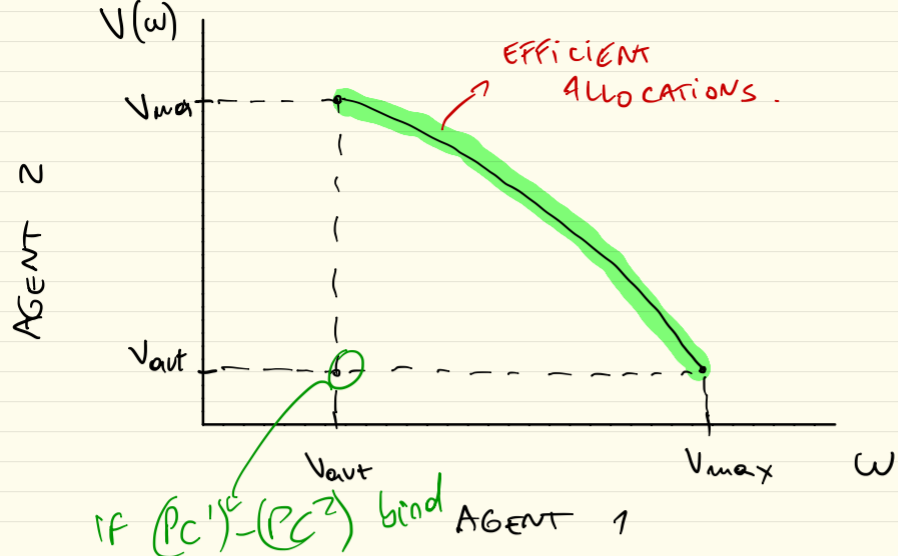
\includegraphics[width=8cm, height=6cm]{pic16}
    \end{center}
    \begin{itemize}
        \item  \underline{First Best Allocation}: an allocation is first best if $c_{t}^{1} + c_{t}^{2} = Y_{t}$ for all dates and states and $u^{'}(c_{t}^{1})/u^{'}(c_{t}^{2})$ is also constant over all dates and states. Therefore, the individual's consumption is a time and state invariant function of the aggregate endowment. Therefore, we solve:
        \begin{gather*}
            V(w) = \max_{c_{s}, w_{s}} \sum_{s=1}^{S} \pi_{s} [u(Y_{s} - c_{s}) + \beta V(w_{s})] \\
            \text{s.t:} \ \ \sum_{s=1}^{S} \pi_{s} [u(c_{s}) + \beta w_{s}] = w
        \end{gather*}
        \begin{itemize}
            \item  \underline{Proof}: writing the Lagrangian we have
            \begin{gather*}
                \sum_{s=1}^{S} \pi_{s} [u(Y_{s} - c_{s}) + \beta V(w_{s})] - \lambda \left\{\sum_{s=1}^{S} \pi_{s} [u(c_{s}) + \beta w_{s}] - w \right\}
            \end{gather*}
            The FOCs of the First Best Allocation includes:
            \begin{gather*}
                \frac{\partial \lambda}{\partial c} = 0 \Rightarrow -\Pi_{s}u^{'}(Y_{s} - c_{s}) + \lambda \Pi_{s} u^{'}(c_{s}) = 0 \\
            \end{gather*}
            Rearranging this we have
            \begin{gather*}
                \frac{u^{'}(Y_{s} - c_{s})}{u^{'}(c_{s})} = \lambda
            \end{gather*}
            This implies full risk sharing with individual consumption only function with average income
        \end{itemize}
        \item \underline{Solution}: the solution will be driven by the pattern of binding PCs where the possible state of the world can be divided into four groups
        \begin{itemize}
            \item  \underline{State 1}: in which $PC_{1}$ binds
            \item  \underline{State 2}: in which $PC_{2}$ binds
            \item  \underline{State 3}: in which neither $PC$ binds
            \item  \underline{State 4}: in which both $PCs$ bind
        \end{itemize}
        Since state 4 never holds if the allocation is efficient only state 1-3 are possibilities
        \begin{itemize}
            \item  \underline{Proof}: suppose that $PC_{1}$ is binding, then $u(c_{s}) + \beta w_{s} = u(y_{s}^{'}) + \beta v_{aut}$. This implies that $c_{s} \leq y_{s}^{1}$ since $w_{s} \geq v_{aut}$
            Suppose that $PC_{2}$ is binding, then $u(Y_{s} - c_{s}) + \beta v(w_{s}) = u(y_{s}^{2}) + \beta v_{aut}$. This implies the following:
            \begin{align*}
                u(Y_{s} - c_{s}) - u(y_{s}^{2}) &= \beta \overbrace{[v_{aut} - v(w_{s})]}^{\leq 0} \\
                u(y_{s} - c_{s}) &\leq u(y_{s}^{2}) \\
                u(Y_{s} - c_{s}) &\leq u(Y_{s} - Y_{s}^{1}) \\
                Y_{s} - c_{s} &\leq Y_{s} - Y_{s}^{1}
            \end{align*}
            Therefore $c_{s} \geq y_{s}^{1}$. \\ \\
            This means that if both participation constraints bind we have $PC^{1} \rightarrow c_{s} \leq y_{s}^{1}$ and $PC^{2} \rightarrow c_{s} \geq y_{s}^{1}$, therefore $c_{s} = y_{s}^{1}$. This implies that $w_{s} = v_{aut}$ and $v(w_{s}) = v_{aut}$, thus both $PCs$ binding is not an efficient solution
        \end{itemize}
        \item \underline{Efficient Allocations}: it can be shown that V is differentiable, decreasing, and concave. This implies the following evolution of promised utility given our states:
        \begin{itemize}
            \item  \underline{State 1 Evolution}: if $PC_{1}$ binds then $w_{s} > w$
            \item  \underline{State 2 Evolution}: if $PC_{2}$ binds then $w_{s} < w$
            \item  \underline{State 3 Evolution}: if neither $PC$ binds then $w_{s} = w$
        \end{itemize}
        This means that, unlike with one-sided commitment, promised values can fall since agents will alter their promised values with eachother in order to achieve insurance under the contract
        \begin{itemize}
            \item  \underline{Proof}: we have the following objective function
            \begin{gather*}
                v(w) = \max_{c_{s}, w_{s}} \sum_{s} \Pi_{s} [u(y_{s} - c_{s}) + \beta v(w_{s})] \\
                \text{s.t:} \ \  \eta \sum_{s} \Pi_{s}[u(c_{s}) + \beta w_{s}] = w \\
                \mu_{s}^{1} u(c_{s}) + \beta w_{s} \geq u(y_{s}^{'}) + \beta v_{aut}, \ \ \ \forall s \\
                \mu_{s}^{2} u(Y_{s} - c_{s}) + \beta v(w_{s}) \geq u(y_{s}^{2}) + \beta v_{aut}, \ \ \ \forall s \\
            \end{gather*}
            Note that $\eta$, $\mu_{s}^{2}$, and $\mu_{s}^{1}$ are arbitrarily attached multipliers. Taking first order conditions and applying the envelope theorem yields the following:
            \begin{align*}
             \frac{\partial v}{\partial w_{s}} = 0 &\rightarrow \Pi_{s} \beta v^{'}(w_{s}) + \eta \Pi_{s} \beta + \mu_{s}^{1} \beta + \mu_{s}^{2} \beta V^{'}(w_{s}) = 0 \tag{1} \\
             \frac{\partial v}{\partial c_{s}} = 0 &\rightarrow - \Pi_{s}u^{'}(Y_{s} - c_{s}) + \eta \Pi_{s}u^{'}(c_{s}) + \mu_{s}^{1}u^{'}(c_{s}) - \mu_{s}^{2} u^{'}(y_{s} - c_{s}) = 0 \tag{2} \\
             \text{Envelope Theorem} &\rightarrow v^{'}(w) = -\eta \tag{3}
         \end{align*}
            We need to consider the 3 states: (1) when $PC_{1}$ binds and therefore $\mu_{s}^{1} > 0, \  \mu_{s}^{2} = 0$, (2) when $PC_{2}$ binds and therefore $\mu_{s}^{1} = 0, \ \mu_{s}^{2} > 0$, (3) no PC binds and therefore $(\mu_{s}^{1} = \mu_{s}^{2} = 0)$
            \begin{itemize}
                \item  \underline{State 1 - $PC_{1}$ Binds}: by $(1)$ and $(3)$ we have
                \begin{gather*}
                    \Pi_{s}v^{'}(w_{s}) \sout{\beta} - v^{'}(w) \Pi_{s} \sout{\beta} + \mu_{s}^{1} \sout{\beta} = 0 \\
                    \big\Updownarrow \\
                    v^{'}(w_{s}) = v^{'}(w) - \frac{\mu_{s}^{1}}{\Pi_{s}}
                \end{gather*}
                Therefore $v^{'}(w_{s}) < v^{'}(w)$ and thus, by concavity, $w_{s} > w$
                \item  \underline{State 2 - $PC_{2}$ Binds}: by rearranging equations $(1)$ and $(3)$ we get
                \begin{gather*}
                    v^{'}(w_{s}) = \frac{\Pi_{s}}{\Pi_{s} + \mu_{s}^{2}} v^{'}(w) \\
                    \Downarrow \\
                    \frac{v^{'}(w_{s})}{v^{'}(w)} = \frac{\Pi_{s}}{\Pi_{s} + \mu_{s}^{2}} < 1 \\
                    \Downarrow \\
                    v_{'}(w_{s}) > v^{'}(w)
                \end{gather*}
                Therefore, $w_{s} < w$
                \item  \underline{State 2 - No PC Binds}: by $(1)$ and $(3)$ we have that $v^{'}(w_{s}) = v^{'}(w)$. Therefore, $w_{s} = w$
            \end{itemize}
        \end{itemize}
        Analogously to what we showed in the one-sided limited commitment model, it follows that:
        \begin{itemize}
            \item  $PC_{1}$ binds when $y_{s}^{1}$ is high
            \item  $PC_{2}$ binds when $y_{s}^{2}$ is high
            \item  $w_{s}$ is a non-decreasing function of $c_{s}$
        \end{itemize}
        Combined with the evolution of promised utilitys this implies that $Cov(c_{t}, y_{t} | Y_{t}) \geq 0$ and therefore we have imperfect risk sharing. Given the correlation result with imperfect risk sharing, lagged individual income occurs since in an efficient allocation $$Cov(c_{t}^{j}, y_{t-k}^{j} | Y_{t-k}) \geq 0$$ for $k \geq 0$ and $j = 1,2$
        \item \underline{Long-Run Dynamics}: suppose the first best allocation is not sustainable. Then as $t \rightarrow \infty$, $\Pr(w_{t} | w_{0})$ converges in distribution to the same non-degenerate limiting distribution for all $w_{0}$.
        As a result the first best is typically not sustainable whenever $\beta$ is small enouggh. This result strengthens the previous result on imperfect risk sharing in two dimensions:
        \begin{itemize}
            \item  \underline{Dimension 1}: it holds in the long run, as the limiting distribution is non-degenerate
            \item  \underline{Dimension 2}: the same distribution (and hence correlation) is obtained regardless of initial promised values
        \end{itemize}
    \end{itemize}
\end{itemize}
\underline{Graphical Intuition for Perpetual Imperfect Risk Sharing}
\begin{center}
\textbf{One Sided Limited Commitment} \par
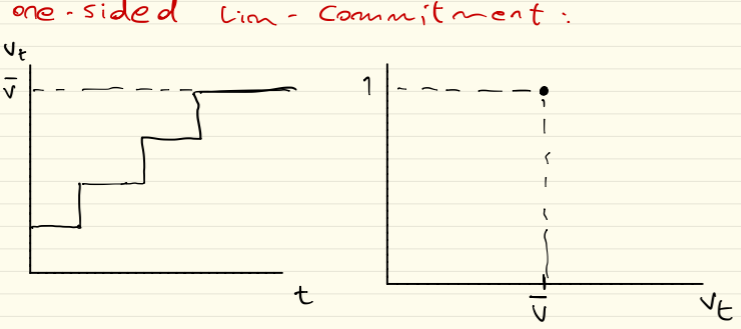
\includegraphics[width=4cm, height=3cm]{pic17}
\end{center}
\begin{center}
\textbf{Two Sided Limited Commitment} \par
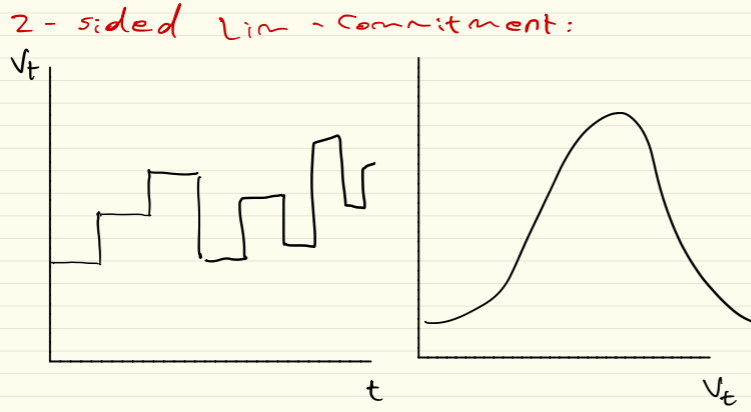
\includegraphics[width=4cm, height=3cm]{pic18}
\end{center}

\newpage

\section{Mirrlees Taxation Model with Two Types}

\vspace{2.5mm}
\par \underline{Variable Overview}: let $y$ denote before-tax income and let $T(y)$ denote the income tax schedule. The optimal income tax system $T^{*}(y)$ is the one that maximizes social welfare subject to a revenue requirement. $T^{*}(y)$ can be found by either the Ramsey approach of Mirrlees approach
\vspace{2.5mm}
\par \underline{Ramsey Approach}: makes parametric assumptions on the tax function $T(y)$ (i.e. a progressive tax function such as $T(y) = y - \lambda y^{1-\tau}$) and precludes non-distortionary lump sum taxes (i.e. $T(y) = constant$ is not allowed)
\begin{itemize}
    \item  \underline{Advantages}: tractability
    \item  \underline{Disadvantages}: the set of possible tax instruments is exogeneous, by precluding lump-sum taxation the taxes are distortionary by assumption, the optimal tax function is arbitrarily restricted
\end{itemize}
\vspace{2.5mm}
\par \underline{Mirrlees Approach}: feasible tax instruments are endogeneised given informational frictions by featuring workers who are traditionally heterogeneous across labour productivity/skill (which are private information). This leads to a trade off between redistribution and work incentives where the right balance in this trade-off will shape tax distortions and hence the optimal tax function $T^{*}(y)$
\begin{itemize}
    \item  \underline{Contractual Friction}: applies tools from contract theory and adverse selection where private information acts as a contractual frictions
    \item  \underline{Static Environments}: involves either a discrete number of different worker skill types or a continuous number of different worker skill types
\end{itemize}

\vspace{2.5mm}
\par \underline{Mirrlees Model with Two Types}: involves a static economy with a single consumption good and a continuum of workers of one of two skill types. No ad-hoc structure on tax design ($T^{*}(y)$) is imposed and the only contraints on $T^{*}(y)$ arise endogenously due to informational frictions. Workers earn money on the basis of their skills and their effort, so there is a tradeoff between effort and taxes the planner applies
\begin{itemize}
    \item  \underline{Assumptions}: $\theta$ and $n$ are private information, $y$ is observable, aggregate output is linear in effective effort (implies that in a competitive equilibrium with a perfect labor market that y equals before tax income), workers have no income effects due to quasi-linear preferences (there are only substitution effects of after-tax  income)
    \item  \underline{Heterogeneity of Workers}: workers are heterogeneous across skills/labor productivity where $\theta \in \Theta$ and $F: \ \Theta \rightarrow [0,1]$ denotes the cumulative distribution function of $\theta$
    \item  \underline{Worker Preferences and Transformation}: workers have quasi-linear preferences over consumption $c$ and effort $n$:
    \begin{gather*}
        U(c,n) = c - v(n)
    \end{gather*}
    where $v^{'}, v^{''} > 0$ (i.e. $v$ is convex). Workers transform effort into output $y$ (or effective labour) using the technology function $y = \theta \cdot n$. Note that $n$ is substituted by $y/\theta$ due to n not being observable, allowing us to write the contract in terms of observables
    \item  \underline{Key Tradeoff}: there is a tradeoff between equity and efficieny. This is as confiscatory taxation improves upon the distribution of the 'social pie' but also reduces production and thus the size of the pie
    \item  \underline{Allocation (the contract)}: an allocation is an assignment of $c$ and $y$ given $\theta$:
    \begin{gather*}
        \left\{ c(\theta), y(\theta) \right\}_{\theta \in \Theta} \ \ \Rightarrow \ \text{the contract}
    \end{gather*}
    This allocation is feasible if and only if
    \begin{gather*}
        \int c(\theta) dF(\theta) + G \leq \int y(\theta) dF(\theta)
    \end{gather*}
    where the LHS is aggregate consumption plus exogenous government expenditure, the RHS is aggregate output.
    \item  \underline{Social Welfare Function}: the government aims to allocate $c$ and $y$ across $\theta$ to maximize the SWF:
    \begin{gather*}
        SWF = \int \Psi \big( c (\theta) - v(\frac{y(\theta)}{\theta}) \big) d F(\theta)
    \end{gather*}
    where $\Psi^{'} > 0$ and $\Psi^{''} < 0$ (ie is increasing and concave). The SWF encapsulates the normative criterion followed by the government and given the concavity of $\Psi$ displays a preference for redistribution across $\theta$s
    \item \underline{Aim}: to design an income tax system that maximizes social welfare. More precisely, let $T(y)$ be the income tax schedule so that agents face the budget constraint $c \leq y - T(y)$. In this case, we are seeking a function $T^{*}(y)$ that maximizes the SWF in a competitive equilibrium and focus on characterising optimal marginal tax rates $T^{*'}(y)$ across the income distribution
    \item  \underline{Solution for Optimal Taxes}: we find $T^{*}(y)$ by following two steps
    \begin{itemize}
        \item  \underline{Step 1 - Centralization (Contract Design)}: characterise the allocations for $\left\{ c^{*}, y^{*} \right\}$ that maximise the SWF subject to informational constraints
        \begin{itemize}
            \item \underline{First Best}: Start by analyzing the case in which the government can observe $\theta$. At this 'first best', the government solves:
            \begin{gather*}
                \max_{\left\{c(\theta), y(\theta) \right\}_{\theta \in \Theta} } \int \Psi \big( c (\theta) - v(\frac{y(\theta)}{\theta}) \big) d F(\theta) \\
                \text{subject to} \\
                \int c(\theta) dF(\theta) + G \leq \int y(\theta) dF(\theta) \tag{RC}
            \end{gather*}
            Assume that the set of possible types (i.e. two) is given by $\Theta = \left\{\theta_{L}, \theta_{H} \right\}$ with $\theta_{L} < \theta_{H}$ and let $\pi_{i} \in (0,1)$ denote the probability of being type $theta_{i}$. Therefore, with two types, the first best becomes:
            \begin{gather*}
                \max_{c_{L}, y_{L}, c_{H}, y_{H}} \sum_{i \in \left\{ L, H \right\} } \pi_{i} \Psi \big( c_{i} - v(\frac{y_{i}}{\theta_{i}})\big) \\
                \text{subject to} \\
                \sum_{i \in \left\{ L,H \right\} } \pi_{i} c_{i} + G \leq \sum_{i \in \left\{ L,H \right\} } \pi_{i} y_{i} \tag{RC}
            \end{gather*}
            It can be shown that at the first best:
            \begin{itemize}
                \item  \underline{Property 1}: everyone gets the same utility, $c_{L}^{FB} - v(\frac{y_{L}^{FB}}{\theta_{L}}) = c_{H}^{FB} - v(\frac{y_{H}^{FB}}{\theta_{H}})$
                \item  \underline{Property 2}: high types work more, $y^{FB}_{H} > y^{FB}_{L}$
            \end{itemize}
            \underline{Issue}: the first best cannot be implemented under private information since high types have incentives to misreport their type
            \begin{itemize}
                \item  \underline{Proof}: using $\theta_{H} > \theta_{L}$ and $y_{H}^{FB} > y_{L}^{FB}$ we get:
                \begin{align*}
                    c_{L}^{FB} - v(\frac{y_{L}^{FB}}{\theta_{H}}) &> c_{L}^{FB} - v(\frac{y_{L}^{FB}}{\theta_{L}}) \\
                    &= c_{H}^{FB} - v(\frac{y_{H}^{FB}}{\theta_{H}^{FB}})
                \end{align*}
                which follows property 1 and implies that if the principal offered the First Best contract, both types of agents would choose $(c_{L}^{FB}, y_{L}^{FB})$. Therefore, there will not be equal utility between types.
            \end{itemize}
            \item  \underline{Second Best}: the principal can generally do better than the first best by screening types. This is done via offering a contract through which different types get different allocations - wherein, under the Revelation Principle, asking agents directly about their types can occur without loss of generality. \\ With the Revelation Principle we add the Incentive Compatibility Contraints ($IC_{H}$ and $IC_{L}$), which requires that individuals should be better-off by revealing their true types. Therefore, the second best problem becomes:
            \begin{gather*}
                \max_{c_{L}, y_{L}, c_{H}, y_{H}} \sum_{i \in \left\{ L, H \right\} } \pi_{i} \Psi \big( c_{i} - v(\frac{y_{i}}{\theta_{i}}) \big) \\
                \text{subject to} \\
                \sum_{i \in \left\{ L,H \right\} } \pi_{i} c_{i} + G \leq \sum_{i \in \left\{ L,H \right\} } \pi_{i} y_{i} \tag{RC} \\
                c_{H} - v(\frac{y_{H}}{\theta_{H}}) \geq c_{L} - v(\frac{y_{L}}{\theta_{H}}) \tag{$IC_{H}$} \\
                c_{L} - v(\frac{y_{L}}{\theta_{L}}) \geq c_{H} - v(\frac{y_{H}}{\theta_{L}}) \tag{$IC_{L}$}
            \end{gather*}
            This is a direct mechanism since allocations are indexed by $\theta$-types. It can be shown that only $IC_{H}$ will be binding at the optimum.
            \begin{itemize}
                \item  \underline{Logic}: this is a reflection of the equity and efficiency tradeoff. Since the redistribution from $\theta_{H}$ to $\theta_{L}$ is desired, $\theta_{H}$ might mimic $\theta_{L}$ and work less (thus decreasing the size of the pie). The binding of $IC_{H}$ means that $\theta_{H}$ should be provided with incentives not to shirk. The ICs effectively are just constraints that a types utility from correctly reporting must be greater than or equal to their utility from misreporting
            \end{itemize}
            Since only $IC_{H}$ is binding, the second best problem becomes:
            \begin{gather*}
                \max_{c_{L}, y_{L}, c_{H}, y_{H}} \sum_{i \in \left\{L, H \right\}} \pi_{i} \Psi \big( c_{i} - v(\frac{y_{i}}{\theta_{i}}) \big) \\
                \text{subject to} \\
                \sum_{i \in \left\{L,H \right\}} \pi_{i} c_{i} + G \leq \sum_{i \in \left\{L,H \right\}} \pi_{i} y_{i} \tag{$\lambda$} \\
                c_{H} - v(\frac{y_{H}}{\theta_{H}}) \geq c_{L} - v(\frac{y_{L}}{\theta_{H}}) \tag{$\mu$}
            \end{gather*}
            where $\lambda, \mu > 0$ and denote the multipliers on $RC$ and $IC_{H}$ respectively.
            \begin{itemize}
                \item  \underline{First Order Conditions}: taking FOCs on the second best problem with $IC_{H}$ binding yields:
                \begin{align*}
                    0 = \frac{\partial U}{\partial c(\theta_{L})} &= \pi(\theta_{L}) \Psi^{'}[c(\theta_{L}) - v(\frac{y(\theta_{L})}{\theta_{L}})] - \lambda \pi(\theta_{L}) - \mu \tag{1} \\
                    0 = \frac{\partial U}{\partial c(\theta_{H})} &= \pi(\theta_{H}) \Psi^{'}[c(\theta_{H}) - v(\frac{y(\theta_{H})}{\theta_{H}})] - \lambda \pi(\theta_{H}) - \mu \tag{2} \\
                    0 = \frac{\partial U}{\partial y(\theta_{L})} &= -\theta(\lambda_{L}) \Psi^{'}[c(\lambda_{L}) - v(\frac{y(\theta_{L})}{\theta_{L}})] v^{'}(\frac{y(\theta_{L})}{\theta_{L}}) \frac{1}{L} + \lambda \pi(\theta_{L}) + \mu v^{'} (\frac{y(\theta_{L})}{\theta_{H}}) \frac{1}{\theta_{H}} \tag{3} \\
                    0 = \frac{\partial U}{\partial y(\theta_{H})} &= -\theta(\lambda_{H}) \Psi^{'}[c(\lambda_{H}) - v(\frac{y(\theta_{H})}{\theta_{H}})] v^{'}(\frac{y(\theta_{H})}{\theta_{H}}) \frac{1}{H} + \lambda \pi(\theta_{H}) + \mu v^{'} (\frac{y(\theta_{H})}{\theta_{H}}) \frac{1}{\theta_{H}} \tag{4}
                \end{align*}
            \end{itemize}
        \end{itemize}
        \item  \underline{Step 2 - Decentralisation}: back out the $T^{*}(y)$ that implement $\left\{ c^{*}, y^{*} \right\}$ as a competitive equilibrium
        \begin{itemize}
            \item  \underline{Framework}: in a decentralised economy an agent of type $\theta$ solves:
            \begin{gather*}
                \max_{c,y} c - v(\frac{y}{\theta}) \\
                \text{subject to} \\
                c = y - T(y)
            \end{gather*}
            This implies that $T^{'}$ satisfies:
            \begin{gather*}
                1 - T^{'}(y) = v^{'}(\frac{y}{\theta}) \frac{1}{\theta} \tag{5}
            \end{gather*}
            This, together with the FOCs, can be used to characterise optimal marginal taxes $T^{*'}(y)$ for $y_{L}$ and $y_{H}$.
            \item \underline{High Skilled Taxation}: recall that
            \begin{gather*}
                1 - T^{*'}(y(\theta_{H})) = v^{'}(\frac{y(\theta_{H})}{\theta_{H}}) \frac{1}{\theta_{H}}
            \end{gather*}
            By equation (2) we have that:
            \begin{gather*}
                \pi(\theta_{H}) \Psi^{'}(\mathcal{U}(\theta_{H})) + \mu = \lambda \pi(\theta_{H}) \tag{2'} \\
                \text{where}: \ \ \mathcal{U}(\theta_{H}) = c(\theta_{H}) - v(\frac{y(\theta_{H})}{\theta_{H}})
            \end{gather*}
            By equation (4) we have that:
            \begin{gather*}
                v^{'}(\frac{y(\theta_{H})}{\theta_{H}}) \frac{1}{\theta_{H}} \big[\pi(\theta_{H})\Psi^{'}(\mathcal{U}(\theta_{H}))+\mu] = \lambda \pi(\theta_{H}) \tag{4'}
            \end{gather*}
            By (2') and (4') we have that:
            \begin{gather*}
                v^{'}(\frac{y(\theta_{H})}{\theta_{H}}) \frac{1}{\theta_{H}} = 1 \tag{*}
            \end{gather*}
            By (5) we have
            \begin{gather*}
                T^{'}(y(\theta_{H})) = 0 \tag{**}
            \end{gather*}
            implying that we have zero marginal taxation at the top.
            \item  \underline{Low Skilled Taxation}: by (1) we have:
            \begin{gather*}
                \lambda \pi(\theta_{L}) = \pi(\theta_{L}) \Psi^{'}(\mathcal{U}(\theta_{L})) - \mu \tag{1'}
            \end{gather*}
            By (3) we have:
            \begin{gather*}
            \lambda \pi (\theta_{L}) = \pi (\theta_{L}) \Psi^{'} (\mathcal{U}(\theta_{L})) v^{'}(\frac{y(\theta_{L})}{\theta_{L}}) \frac{1}{\theta_{L}} - \mathcal{U} v^{'} (\frac{y(\theta_{L})}{\theta_{H}}) \frac{1}{\theta_{H}} \tag{3'}
            \end{gather*}
            Combining (1') and (3') yields:
            \begin{gather*}
                \pi(\theta_{L}) \Psi^{'}(\mathcal{U}(\theta_{L})) - \mu = \pi(\theta_{L}) \Psi^{'} (\mathcal{U}(\theta_{L})) v^{'}(\frac{y(\theta_{L})}{\theta_{L}}) \frac{1}{\theta_{L}} - \mu v^{'} (\frac{y(\theta_{L})}{\theta_{H}}) \frac{1}{\theta_{H}} \\
                \text{which is equivalent to} \\
                \pi(\theta_{L}) \Psi^{'}(\mathcal{U}(\theta_{L})) \underbrace{\big[1 - v^{'}(\frac{y(\theta_{L})}{\theta_{L}}) \frac{1}{\theta_{L}} \big]}_{\begingroup\color{cyan} \equiv T^{'}(y(\theta_{L})) \endgroup} = \mu \big[1 - v^{'}(\frac{y(\theta_{L})}{\theta_{H}}) \frac{1}{\theta_{H}} \big]
            \end{gather*}
            Rearranging this and inserting $+/- \mu v^{'}(\frac{y(\theta_{H})}{\theta_{H}}) \frac{1}{\theta_{H}}$ we have:
            \begin{align*}
                T^{'}(y(\theta_{L})) &= \mu \big[1 - v^{'}(\frac{y(\theta_{L})}{\theta_{H}}) \frac{1}{\theta_{H}} \big] \frac{1}{\pi(\theta_{L}) \Psi^{'}(u(\theta_{L}))} \\
                T^{'}(y(\theta_{L})) &= \mu \big[\underbrace{1 - v^{'}(\frac{y(\theta_{H})}{\theta_{H}}) \frac{1}{\theta_{H}}}_{\begingroup\color{magenta} \equiv 0 \ \ \text{by (**)}\endgroup} + v^{'}(\frac{y(\theta_{H})}{\theta_{H}})\frac{1}{\theta_{H}} - v^{'}(\frac{y(\theta_{L})}{\theta_{H}})\frac{1}{\theta_{H}} \big] \frac{1}{\pi(\theta_{L}) \Psi^{'}(u(\theta_{L}))} \\
                T^{'}(y(\theta_{L})) &= \mu \big[ v^{'}(\frac{y(\theta_{H})}{\theta_{H}})\frac{1}{\theta_{H}} - v^{'}(\frac{y(\theta_{L})}{\theta_{H}})\frac{1}{\theta_{H}} \big] \frac{1}{\pi(\theta_{L}) \Psi^{'}(u(\theta_{L}))} \tag{**}
            \end{align*}
            Note that since $y(\theta_{H}) \geq y(\theta_{L})$, ** must be positive. Therefore, $0 \leq T^{'}(y(\theta_{L})) \leq 1$
        \end{itemize}
        \item  \underline{Summary}: optimal marginal taxes satisfy (A): $T^{*'}(y_{h}) - 0$ and (B): $0 \leq T^{'}(y(\theta_{L})) \leq 1$. Overall, high incomes are untaxed at the margin but low incomes are levied a positive marginal tax (optimal income tax is therefore regressive)
        \begin{itemize}
            \item \underline{Proof}: (A) follows from combining (2), (4), and (5). (B) follows from combining (1), (3), (5), and that $y(\theta_{H}) \geq y(\theta_{L})$
            \item  \underline{Intuition}: there should be no taxation at the top since the distribution of skills is bounded - therefore, a marginal tax on the highest type would only decrease work incenstives without yielding additional revenue. The tax should be regressive to prevent the high type from deviating, so the planner distorts the low type at the margin
        \end{itemize}
    \end{itemize}
\end{itemize}

\newpage
\section{Mirrless Taxation Model with a Continuum of Types}
\vspace{2.5mm}
\par \underline{Setup}: involves a static economy with a single consumption good and a continuum of workers of a continuum of skill types. No ad-hoc structure on tax design ($T^{*}(y)$) is imposed and the only contraints on $T^{*}(y)$ arise endogenously due to informational frictions.
\\ \underline{Assumptions}: $\theta$ and $n$ are private information, $y$ is observable, aggregate output is linear in effective effort (implies that in a competitive equilibrium with a perfect labor market that y equals before tax income)
\underline{Heterogeneity of Workers}: workers are heterogeneous across skills/labor productivity where $\theta \in \Theta$ and $F: \ \Theta \rightarrow [0,1]$ denotes the cumulative distribution function of $\theta$. Here $\Theta = [\theta_{LB}, \theta_{UB}] \rightarrow \ \text{continuum of types}$, wherein $\theta_{UB}$ can be finite or infinite (unbounded distribution)
\\ \underline{Worker Preferences and Transformation}: workers have quasi-linear preferences over consumption $c$ and effort $n$:
\begin{gather*}
    U(c,n) = c - v(n)
\end{gather*}
where $v^{'}, v^{''} > 0$. Workers transform effort into output $y$ (or effective labour) using the technology function $y = \theta \cdot n$. Note that $n$ is substituted by $y/\theta$, allowing us to write the contract in terms of observables
\\ \underline{Key Tradeoff}: there is a tradeoff between equity and efficieny. This is as confiscatory taxation improves upon the distribution of the 'social pie' but also reduces production and thus the size of the pie
\\ \underline{Allocation}: an allocation is an assignment of $c$ and $y$ given $\theta$:
\begin{gather*}
    \left\{ c(\theta), y(\theta) \right\}_{\theta \in \Theta} \ \ \Rightarrow \ \text{the contract}
\end{gather*}
This allocation is feasible if and only if
\begin{gather*}
    \int c(\theta) dF(\theta) + G \leq \int y(\theta) dF(\theta)
\end{gather*}
where the LHS is aggregate consumption plus exogenous government expenditure, the RHS is aggregate output.
\\ \underline{Social Welfare Function}: the government aims to allocate $c$ and $y$ across $\theta$ to maximize the SWF:
\begin{gather*}
    SWF = \int \Psi \big( c (\theta) - v(\frac{y(\theta)}{\theta}) \big) d F(\theta)
\end{gather*}
where $\Psi^{'} > 0$ and $\Psi^{''} < 0$. The SWF encapsulates the normative criterion followed by the government and given the concavity of $\Psi$ displays a preference for redistribution across $\theta$s
\\ \underline{Aim}: to design an income tax system that maximizes social welfare. More precisely, let $T(y)$ be the income tax schedule so that agents face the budget constraint $c \leq y - T(y)$. In this case, we are seeking a function $T^{*}(y)$ that maximizes the SWF in a competitive equilibrium and focus on characterising optimal marginal tax rates $T^{*'}(y)$ across the income distribution
\\ \underline{Solution for Optimal Taxes}: we find $T^{*}(y)$ by following two steps
\\ \underline{Step 1 - Contract Design}: characterise the allocations for $\left\{ c^{*}, y^{*} \right\}$ that maximise the SWF subject to informational Constraints
\begin{itemize}
    \item \underline{Planning Problem}: the social planner solves:
    \begin{gather*}
        \max_{\left\{ c(\theta), y(\theta) \right\}} \int \Psi  \big( c(\theta) - v(\frac{y(\theta)}{\theta}) \big) \\
        \text{subject to}
        \int c(\theta) d F(\theta) \leq \int y(\theta) d F(\theta) \tag{RC} \\
        c(\theta) - v(\frac{y(\theta)}{\theta}) \geq c(\theta^{'}) - v (\frac{y(\theta^{'})}{\theta}), \ \ \forall (\theta, \theta^{'}) \tag{IC}
    \end{gather*}
    \item  \underline{Double Infinite IC Constraints}: as we have a continuum number of types we have an infinite number of $\theta$s, since for each $\theta$ we also have an infinite number of constraints (i.e. $\theta$s to compare to) we therefore have a double infinite number of IC constraints.
    \item  \underline{IC Constraints Simplification}: due to there being a double infinite number of ICs, they must be simplified to characterise the solution. The double infinite series of ICs is simplified by the proposition that (IC) holds if and only if for all $\theta$:
    \begin{gather*}
        c^{'}(\theta) - v^{'}(\frac{y(\theta)}{\theta}) \frac{y^{'}(\theta)}{\theta} = 0 \tag{$IC_{1}$} \\
        \text{and} \\
        y^{'}(\theta) \geq 0 \tag{$IC_{2}$}
    \end{gather*}
    which are the simplified IC constraints
    \begin{itemize}
        \item  \underline{Proof}: the idea of the proof is to show that under $(IC_{1})$ and $(IC_{2})$ we have that $\mathcal{U}(\theta^{'}; \theta) = c(\theta^{'}) - v(\frac{y(\theta^{'})}{\theta})$ attains a global maximum at $\theta^{'} = \theta$ for all $\theta$. Let
        \begin{gather}
            \mathcal{U} (\theta^{'}; \theta) = c(\theta^{'}) - v(\frac{y(\theta')}{\theta})
        \end{gather}
        be the utility of agent $\theta$ from reporting as $\theta^{'}$. This involves proving lemma 1 and then lemma 2
        \item \underline{First Lemma:} \textit{a local maximum of $\mathcal{U}(\theta^{'}; \theta)$ at $\theta^{'} = \theta$ is attained if and only if $\forall \theta \in \Theta$ $(IC_{1})$ and $(IC_{2})$ hold}
        \begin{itemize}
            \item \underline{Lemma 1 Proof}: The first order conditions for local maximum are $$\frac{\partial \mathcal{U}(\theta^{'};\theta)}{\partial \theta^{'}} |_{\theta^{'} = \theta} = 0$$ More succinctly, by $\mathcal{U}_{1}(\theta; \theta) = 0$ and recalling that $\mathcal{U}(\theta^{'}; \theta) = c(\theta^{'}) - v(\frac{y(\theta^{'})}{\theta})$ we have $$\mathcal{U}_{1}(\theta^{'}; \theta) = \underbrace{c^{'}(\theta^{'}) - v^{'}(\frac{y(\theta^{'})}{\theta})\frac{y^{'}(\theta^{'})}{\theta} = 0}_{IC_{1}}$$
            \newline
            The second order conditions for a local maximum at $\theta^{'} = \theta$ are:
            \begin{gather*}
                \frac{\partial^{2} \mathcal{U}(\theta^{'}; \theta)}{\partial \theta^{'2}}|_{\theta^{'} = \theta} \leq 0
            \end{gather*}
            Which can be written as
            \begin{gather}
                \mathcal{U_{11}} (\theta; \theta) \leq 0 \tag(1)
            \end{gather}
            Recall that we showed at a local maximum that $\mathcal{U}_{1}(\theta; \theta) = 0$ and therefore $\mathcal{U}_{11}(\theta; \theta) \leq 0$. Differentiating this with respect to $\theta$ we have
            \begin{gather*}
                \mathcal{U}_{11}(\theta; \theta) + \mathcal{U}_{12}(\theta; \theta) = 0 \tag{2}
            \end{gather*}
            This is as the total derivative is equal to the sum of partial derivatives and the total second order derivative equals 0 at a critical value (e.g. a local minima). By (1) we must then have that $\mathcal{U}_{12}(\theta; \theta) \geq 0$
            \newline
            Expanding on the LHS of (2) and recalling that $\mathcal{U}_{1}(\theta^{'}; \theta) = c^{'}(\theta^{'}) - v^{'}(\frac{y(\theta^{'})}{\theta^{'}})\frac{y^{'}(\theta^{'})}{\theta} = 0$ we have
            \begin{align*}
                \underbrace{\mathcal{U}_{12}(\theta; \theta)}_{\geq 0 \ \text{by (2)}} &= v^{''}(\frac{y(\theta}{\theta}) \frac{y(\theta)}{\theta^{2}} \frac{y^{'}(\theta)}{\theta} + v^{'}(\frac{y(\theta)}{\theta})\frac{y^{'}(\theta)}{\theta^{2}} \\
                &= \underbrace{\big[ v^{''} (\frac{y(\theta)}{\theta}) \frac{y(\theta)}{\theta^{3}} + v^{'}(\frac{y(\theta)}{\theta})\frac{1}{\theta^{2}} \big]}_{\geq 0} y^{'}(\theta)
            \end{align*}
            This implies that $y^{'}(\theta) \geq 0$ ($IC_{2}$)
        \end{itemize}
        \item \underline{Second Lemma:} \textit{ a global maximum of $\mathcal{U}(\theta^{'}; \theta)$ at $\theta^{'} = \theta$ is attained at $\theta^{'} = \theta$ if and only if $\forall \theta \in \Theta$ $(IC_{1})$ and $(IC_{2})$ hold}
        \begin{itemize}
            \item \underline{Lemma 2 Proof}: the idea is to show that the sign of $\mathcal{U}_{1}(\theta^{'}, \theta)$ is the same as $(\theta^{'} - \theta)$
            \newline
            \begin{center}
                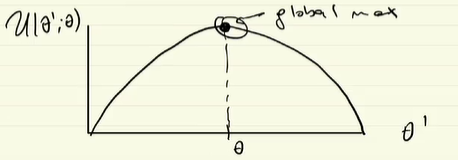
\includegraphics[width=8cm, height=6cm]{pic29}
            \end{center}
            Here we show that the sign of $\mathcal{U}_{1}(\theta^{'};\theta)$ is the same as $(\theta - \theta^{'})$ (which is greater or equal to zero). First note that
            \begin{gather*}
                \mathcal{U}_{1}(\theta^{'}; \theta) = c^{'}(\theta^{'}) - v^{'}(\frac{y(\theta^{'})}{\theta^{'}})\frac{y^{'}(\theta^{'})}{\theta} \tag{i}
            \end{gather*}
            By condition ($IC_{1}$) evaluated at $\theta^{'}$ we have:
            \begin{gather*}
                c^{'}(\theta^{'}) = v^{'}(\frac{y(\theta^{'})}{\theta^{'}})\frac{y^{'}(\theta^{'})}{\theta^{'}} \tag{ii}
            \end{gather*}
            Combining (i) and (ii) yields:
            \begin{align*}
                \mathcal{U}_{1}(\theta^{'}; \theta) &= v^{'}(\frac{y(\theta^{'})}{\theta^{'}})\frac{y^{'}(\theta^{'})}{\theta^{'}} - v^{'}(\frac{y(\theta^{'})}{\theta})\frac{y^{'}(\theta)}{\theta} \\
                &= \underbrace{\big[v^{'}(\frac{y(\theta^{'})}{\theta^{'}}) \frac{1}{\theta^{'}} - v^{'}(\frac{y(\theta^{'})}{\theta})\frac{1}{\theta} \big]}_{\geq 0 \ \text{by} \ (IC_{2})} y^{'}(\theta^{'}) \tag{$[\cdot]$}
            \end{align*}
            By ($IC_{2}$) and because $v^{''} \geq 0$ (i.e. since we have convexity in $v$), we get the following:
            \begin{gather*}
                \text{sign} \ (\mathcal{U_{1}}(\theta^{'},\theta)) = \ \text{sign} \ ([\cdot]) = \ \text{sign} \ (\theta - \theta^{'})
            \end{gather*}
        \end{itemize}
    \end{itemize}
    This proposition has the advantage of reducing dimensionality (from double infinity to infinity constraints) since ($IC_{1}$) and ($IC_{2}$) are conditions for local maxima and therefore we actually work with a local version of ($IC$).
    \item  \underline{Simplified IC Qualities}: ($IC_{2}$) requires that higher types work more. ($IC_{1}$) requires that higher types get higher utility at the optimum.
    \begin{itemize}
        \item  \underline{Proof}: let $\mathcal{U}^{'}(\theta) \equiv U(\theta; \theta)$ be the utility for type $\theta$ at the optimum. Note that
        \begin{gather*}
            \mathcal{U}^{'}(\theta) = \underbrace{\big[c^{'}(\theta) - v^{'}(\frac{y(\theta)}{\theta}) \frac{y^{'}(\theta)}{\theta}\big] }_{\begingroup\color{cyan} = 0 \ by \ (IC_{1}) \endgroup\color{cyan}} + \underbrace{ v^{'} (\frac{y(\theta)}{\theta}) \frac{y(\theta)}{\theta^{2}}}_{\begingroup\color{magenta} \geq 0 \endgroup\color{magenta}}
        \end{gather*}
        Hence, $\mathcal{U}^{'}(\theta) \geq 0$. Note that the above is derived by solving the simplified $IC_{1}$ and substituting it into the utility formula
        \item  \underline{Intuition}: $\mathcal{U}(\lambda)$ should increase with $\lambda$ to incentivise high types to work at full potential. More technically, we need that the informational rent (embedded in $\mathcal{U}(\lambda)$) increases with $\lambda$. These results extend what we obtained in the 2-types case
    \end{itemize}
    \item  \underline{Final Planning Problem} let $\mathcal{U} = c(\theta) - v(\frac{y(\theta)}{\theta})$ be the utility of agent $\theta$ at the optimum. WE can therefore rewrite the planning problem using $\mathcal{U}(\theta)$ as a state variable where:
    \begin{itemize}
        \item  \underline{Consumption}: can be written as $c(\theta) = \mathcal{U}(\theta) + v(\frac{y(\theta)}{\theta})$
        \item  \underline{$IC_{1}$}: is equivalent to $\mathcal{U}^{'}(\theta) = v^{'}(\frac{y(\theta)}{\theta})\frac{y(\theta)}{\theta^{2}}$
    \end{itemize}
    Therefore, the planning problem can be rewritten as:
    \begin{gather*}
        \max_{\left\{ \mathcal{U}(\theta), y(\theta)\right\}_{\theta \in \Theta}} \int \Psi (\mathcal{U}(\theta))f(\theta) d \theta \\
        \text{subject to} \\
        \int \big(\overbrace{\mathcal{U}(\theta) + v(\frac{y(\theta)}{\theta})}^{ \equiv c(\theta)} - y(\theta) \big) f(\theta) d \theta = 0 \tag{RC} \\
        \mathcal{U}^{'}(\theta) = v^{'}(\frac{y(\theta)}{\theta}) \frac{y(\theta)}{\theta^{2}}, \ \ \forall \theta \tag{$IC_{1}$} \\
        y^{'}(\theta) \geq 0, \ \ \forall \theta \tag{$IC_{2}$}
    \end{gather*}
    \item  \underline{Relaxing the Planning Problem}: by applying optimal control techniques we can handle the inequality contraint ($IC_{2}$) and integral constraint (RC)
    \begin{itemize}
        \item  \underline{Inequality Constraint ($IC_{2}$)}: to make progress we neglect the monotonicity condition by assuming it holds at the optimum - thus working with a 'relaxed' planning problem by ignoring ($IC_{2}$)s existence. This is equivalent to assuming that there is no bunching at the optimum (i.e. different types are offered a different contract)
        \newline
        This is the so called 'first-order approach' to the planning problem because ($IC_{1}$), the condition we keep, is a first order condition for truth telling to be optimal while ($IC_{2}$) came from second order conditions. In practice, we typically verify $(IC_{2})$ ex-post via simulations
        \item  \underline{Integral Constraint (RC)}: for applying the Maximum Principle, the constraint set should only include differential equations, not integral constraints. To do this, we define a new state variable $z(\theta)$ such that $z(\theta_{LB}) = z(\theta_{UB}) = 0$ and $z^{'}(\theta) = \underbrace{\big(\mathcal{U}(\theta) + v(\frac{y(\theta)}{\theta}) - y(\theta) \big) f(\theta)}_{\text{integrand of RC}}$. Clearly these conditions are equivalent to the RC, therefore:
        \begin{gather*}
            0 = z(\theta_{UB}) - z(\theta_{LB}) = \int_{\theta_{LB}}^{\theta_{UB}} z'(\theta) d \theta = \int_{\theta_{LB}}^{\theta_{UB}} \big( \mathcal{U}(\theta) + v \frac{y(\theta)}{\theta} - y(\theta) \big) f(\theta) d \theta
        \end{gather*}
        \item  \underline{Relaxed Problem}: by handling (RC) and ($IC_{2}$), the relaxed problem becomes:
        \begin{gather*}
            \max_{\left\{ \mathcal{U}(\theta), y(\theta)\right\}_{\theta \in \Theta}} \int \Psi (\mathcal{U}(\theta))f(\theta) d \theta \\
            \text{subject to} \\
            z^{'}(\theta) = \big(\mathcal{U}(\theta) + v(\frac{y(\theta)}{\theta}) - y(\theta) \big) f(\theta), \ \forall \theta \tag{$\lambda, \ RC$} \\
            \mathcal{U}^{'}(\theta) = v^{'}(\frac{y(\theta)}{\theta}) \frac{y(\theta)}{\theta^{2}}, \ \forall \theta \tag{$\mu, \ IC_{1}$} \\
            z(\theta_{LB}) = z(\theta_{UB}) = 0
        \end{gather*}
    \end{itemize}
    \item  \underline{Solving the Relaxed Problem}: this can be done via applying the Maximum Principle with $y(\theta)$ as the control variable and $z(\theta), \mathcal{U}(\theta)$ as the state Variables. The Hamiltonian is:
    \begin{gather*}
        H = \Psi (\mathcal{U}(\theta)) f(\theta) + \lambda (\theta) \big[\mathcal{U}(\theta) + v(\frac{y(\theta)}{\theta}) - y(\theta) \big] f(\theta) + \mu (\theta) v^{'} (\frac{y(\theta)}{\theta}) \frac{y(\theta)}{\theta^{2}}
    \end{gather*}
    where $\lambda (\theta)$ and $\mu (\theta)$ are the costates associated with $z(\theta)$ and $\mathcal{U}(\theta)$. According to the Maximum Principle, the necessary consitions for an optimum are (dropping explicit dependencies on $\theta$):
    \begin{align*}
        \frac{\partial H}{\partial y} &= 0 \ \Rightarrow \ H_{y} = \lambda \big[v^{'}(\frac{y}{\theta}) \frac{1}{\theta} - 1 \big]f + \mu \big[v^{''}(\frac{y}{\theta})\frac{1}{\theta^{3}} + v^{'}(\frac{y}{\theta}) \frac{1}{\theta^{2}} \big] = 0\\
        \frac{\partial H}{\partial z} &= -\lambda^{'} \Rightarrow \lambda^{'} = 0 \\
        \frac{\partial H}{\partial \mathcal{U}} &= -\mu^{'} \Rightarrow \mu^{'} = - \big[\Psi^{'}(\mathcal{U}) + \lambda \big] f
    \end{align*}
    Boundary conditions are (recall that $\mathcal{U}$ is free at the boundaries):
    \begin{gather*}
        \mu(\theta_{LB}) = \mu(\theta_{UB}) = 0
    \end{gather*}
    \begin{itemize}
        \item  \underline{Disutility of Effort}: the disutility for effort is isoelastic $$v(n) = \frac{n^{1+\tfrac{1}{\varepsilon}}}{1 + \tfrac{1}{\varepsilon}}$$ where $\varepsilon > 0$ is the Frisch elasticity of labour supply and measures the elasticity of effort to a change in wages, holding constant the marginal utility of wealth
        \item  \underline{Average Marginal SW}: let $$D(\theta) \equiv \frac{1}{1 - F(\theta)} \int_{\theta_{LB}}^{\theta_{UB}} \Psi^{'} (\mathcal{U}(\widetilde{\theta})) f (\widetilde{\theta}) d \widetilde{\theta} $$ be the average marginal social welfare weight on individuals with $\widetilde{\theta} \geq \theta$
        \begin{itemize}
            \item $\underline{D(\theta)}$: summarises the redistributive tastes of the planner where $D(\theta) \geq 0$ and is decreasing in $\theta$ by the concavity of $\Psi$
            \item \underline{Note}: $F(\theta)$ is the proportion of agents with skill type $\theta \leq \widetilde{\theta}$ and will increase as $\widetilde{\theta}$ increases. This implies a higher social weight on individuals with higher $\widetilde{\theta}$ and therefore that they should be taxed less (all else equal). Further note that $(1 - F(\theta)) = \int_{\theta - \theta_{LB}} f(\theta) d \theta$
        \end{itemize}
    \end{itemize}
    \item \underline{Optimal Marginal Taxes}: the optimal marginal taxes satisfy $$\frac{T^{*'}(y^{*}(\theta))}{1 - T^{*'}(y^{*}(\theta))} = (1 + \frac{1}{\varepsilon})(1 - \frac{D(\theta)}{D(\theta_{LB})})\frac{1 - F(\theta)}{\theta f(\theta)}$$ This has three key determinants: (1) elasticity of labour supply, (2) redistributive tastes, (3) distribution of skills. Recall that $y^{'} \geq 0$.
    \begin{itemize}
        \item  \underline{Proof Step 1 - Centralization}: characterise the allocations for $\{ c^{*}, y^{*} \}$ that maximise the SWF subject to informational constraints using the planning problem. \\
        By the maximum principal we have:
        \begin{gather*}
            \lambda [v^{'} (\frac{y}{\theta})\frac{1}{\theta}-1]f + \mu [v^{''}(\frac{y}{\theta})\frac{y}{\theta^{3}} + v^{'}(\frac{y}{\theta})\frac{1}{\theta^{2}}] = 0 \tag{1} \\
            \lambda^{'} = 0 \tag{2} \\
            \mu^{'} = -[\Psi^{'}(\mathcal{U}) + \lambda]f \tag{3}
        \end{gather*}
        Recall that $\mathcal{U}$ is free at the boundaries so $\mu(\theta_{LB}) = \mu(\theta_{UB}) = 0$. Therefore, by integrating (3) over all $\theta$ we have:
        \begin{gather*}
            \underbrace{\int_{\theta_{LB}}^{\theta_{UB}} \mu^{'}(\widetilde{\theta}) d \widetilde{\theta}}_{\mu(\theta_{UB}) - \mu(\theta_{LB}) = 0} = -\int_{\theta_{LB}}^{\theta_{UB}} [\Psi^{'} (\mathcal{U}(\widetilde{\theta})) + \lambda]f(\widetilde{\theta}) d \widetilde{\theta} \tag{4}
        \end{gather*}
        Based on (4), we have that:
        \begin{align*}
            \lambda' &= - \int_{\theta_{LB}}^{\theta_{UB}} \Psi^{'} (\mathcal{U}(\widetilde{\theta}))f(\widetilde{\theta})d \widetilde{\theta} \\
            \lambda' &= -D(\theta_{LB}) \tag{5}
        \end{align*}
        Since when $\widetilde{\theta} = \theta_{LB}$ we have that $(1 - F(\theta) = 1$, yielding the above result. Also, by integrating (3) between $[\theta, \theta_{UB}]$ we get:
        \begin{gather*}
            \underbrace{\mu(\theta_{UB})}_{=0} - \mu(\theta) = - \int_{\theta}^{\theta_{UB}} [\Psi^{'} (\mathcal{u}(\widetilde{\theta})) + \lambda]f (\widetilde{\theta}) d \widetilde{\theta} \\
            \mu(\theta) =  \underbrace{\int_{\theta}^{\theta_{UB}} [\Psi^{'} (\mathcal{u}(\widetilde{\theta}))]f (\widetilde{\theta}) d \widetilde{\theta}}_{(1 - F(\theta))D(\theta)} +  \underbrace{\lambda}_{-D(\theta_{LB})}  \underbrace{\int_{\theta}^{\theta_{UB}} f (\widetilde{\theta}) d \widetilde{\theta}}_{1 - F(\theta)}
        \end{gather*}
        Therefore, we have that:
        \begin{gather*}
            \mu (\theta) = (1-F(\theta)) (D(\theta) - D(\theta_{LB})) \tag{6}
        \end{gather*}
        Note that $\mu(\theta) \leq 0$ since $(D(\theta) - D(\theta_{LB})) \leq 0$ as $D(\theta)$ is decreasing in $\theta$ (based on the planner's taste for redistribution). Using the functional form for $v(\cdot)$ we have:
        \begin{gather*}
            v(n) = \frac{n^{1+\tfrac{1}{\varepsilon}}}{1 + \tfrac{1}{\varepsilon}} \\
            \therefore v^{'}(n) = n^{\tfrac{1}{\varepsilon}} \tag{7} \\
            \therefore v^{''}(n) = \frac{1}{\varepsilon} n^{\tfrac{1}{\varepsilon} -1} \tag{7}
        \end{gather*}
        Using (5), (6), and (7) into (1), we get:
        \begin{gather*}
            \underbrace{D(\theta_{LB})}_{\lambda} [(\frac{y}{\theta})^{\tfrac{1}{\varepsilon}} \frac{1}{\theta} - 1] f(\theta) = \underbrace{(1 - F(\theta))(D(\theta) - D(\theta_{LB}))}_{\mu(\theta)} [\frac{1}{\varepsilon} (\frac{y}{\theta})^{\tfrac{1}{\varepsilon} - 1} \frac{y}{\theta^{3}} + (\frac{y}{\theta})^{\tfrac{1}{\varepsilon}} \frac{1}{\theta^{2}}] \\
            \underbrace{(\frac{y}{\theta})^{\frac{1}{\varepsilon}} \frac{1}{\theta} - 1}_{-T^{'}(y)} = \frac{1 - F(\theta)}{\theta f (\theta)} (\frac{D(\theta)}{D(\theta_{LB})} - 1) (\frac{1}{\varepsilon} + 1) \underbrace{(\frac{y}{\theta})^{\tfrac{1}{\varepsilon}} \frac{1}{\theta}}_{1 - T^{'}(y)} \tag{8}
        \end{gather*}
        (8) can be used in conjunction with the decentralization step to solve for the optimal tax formula
        \item  \underline{Proof Step 2 - Decentralisation}: back out the $T^{*}(y)$ that implement $\left\{ c^{*}, y^{*} \right\}$ as a competitive equilibrium using the individual problem. \\
        The individual solves the following problem in the decentralization
        \begin{gather*}
            \max_{y} \ \underbrace{y - T(y)}_{c} - \underbrace{(\frac{y}{\theta})^{1 + \frac{1}{\varepsilon}} \frac{1}{1 + \tfrac{1}{\varepsilon}}}_{v(\tfrac{y}{\theta})}
        \end{gather*}
        The first order conditions to this problem are:
        \begin{gather*}
            1 - T^{'}(y) = (\frac{y}{\theta})^{\tfrac{1}{\varepsilon}} \frac{1}{\theta} \tag{9}
        \end{gather*}
        By combining (8) and (9) we derive the optimal tax formula
        \begin{gather*}
            \frac{T^{*'}(\theta)}{1 - T^{*'}(\theta)} = (1 + \frac{1}{\varepsilon}) (1 - \frac{D(\theta)}{D(\theta_{LB})}) \frac{1 - F(\theta)}{\theta f(\theta)}
        \end{gather*}
    \end{itemize}
\end{itemize}
\underline{Characteristics of $T^{*'}$}: (1) $T^{*'}(\theta)$ decreases with $\varepsilon$ since large $\varepsilon$ means that marginal taxes create large distortions, (2) $T^{*'}$ decreases with $D(\theta)$ since more social weight on individuals with $\widetilde{\theta} \geq \theta$ implies that the government taxes such individuals less, (3) $T^{*'}$ increases with $\frac{1 - F(\theta)}{\theta f(\theta)}$
\begin{itemize}
    \item  \underline{Logic for (3)}: suppose you increase $T^{*'}$. Then, all else equal, the government collects more tax revenue on individuals above $\theta$, who are $(1 - F(\theta))$ in number. This explains the positive dependence on $(1 - F(\theta))$. However, the resulting distortion is proportional to the mass of individuals at $\theta$ and to their productivity level $\theta$. This explains the negative dependence on $\theta f (\theta)$
\end{itemize}
\vspace{2.5mm}
\par \underline{Quantifying Optimal Taxes}: optimal marginal taxes satisfy $\frac{T^{*'}(\theta)}{1 - T^{*'}(\theta)} = (1 + \frac{1}{\varepsilon}) (1 - \frac{D(\theta)}{D(\theta_{LB})}) \frac{1 - F(\theta)}{\theta f(\theta)}$ with its key determinants being (1) elasticity of labour supply, (2) redistributive tastes, (3) distribution of skills
\begin{itemize}
    \item  \underline{Elasticity of Labour Supply ($\varepsilon$)}: $\varepsilon$ can be estimated from the data which suggests that the reasonable range among US males is $\varepsilon \in [0,0.5]$ and for US females $\varepsilon \geq 0.5$
    \item  \underline{Redistributive Tastes ($D(\theta)$)}: the shape of $D(\theta)$ is driven by the parameterisation of $\Psi$, typically the 'weighted utilitarian' SWF is used: $$\Psi(\mathcal{U}(\theta)) = a(\theta)\mathcal{U}(\theta) \Rightarrow D(\theta) = \frac{1}{1 - F(\theta)} \int_{\theta}^{\theta_{UB}} a(\widetilde{\theta})f(\widetilde{\theta}) d \widehat{\theta}$$ where $a(\theta)$ decreases with $\theta$. The Rawlsian $a(\theta_{LB}) = + \infty$ and Utilitarian $a(\theta) = 1$ for all $\theta$
    \item  \underline{Skill Distribution $f(\theta)$}: given the issue of the distribution of skills being unobservable, there are two common approaches - (1) the Saez approach backs out distribution of skills from distribution of income, (2) the Mankiw approach proxies skills with wages
    \begin{itemize}
        \item  \underline{Distribution of Skills}: if the distribution of skills is bounded then $\frac{1 - F(\theta_{UB})}{\theta_{UB}f (\theta_{UB})} = 0$ so that $T^{*'}(\theta_{UB}) = 0$ as in the two type model. However, if the distribution of skills is unbounded then this is not the case
    \end{itemize}
\end{itemize}
\vspace{2.5mm}
\par \underline{Saez Approach to Skill Distribution Analysis}: suppose that given the actual tax schedule $T(y)$ we observe an income distribution with cdf $Q(y)$. As long as $y^{'}(\theta) \geq 0$, we can back out the skill distribution based on the relationship $F(\theta) = Q(y(\theta))$. This implies that $f(\theta) = q (y(\theta))y^{'}(\theta)$, where $y^{'}(\theta)$ on the RHS can be recovered from the utility maximization problem given the actual tax code
\begin{itemize}
    \item  \underline{Optimization Problem}: given the actual tax code $T$, the agent solves
    \begin{gather*}
        \max_{c,y} c - v(\frac{y}{\theta}) \\
        \text{Subject to:} \ c = y - T(y)
    \end{gather*}
    The first order conditions of this problem imply that $$1 - T^{'}(y) - v^{'}(\frac{y}{\theta})\frac{1}{\theta} = 0$$ This implicity defines $y(\theta)$ and $y^{'}(\theta)$. Therefore, we can identify the skill distribution from the distribution of observed incomes and the observed tax schedule
    \item  \underline{Skill Distribution at the Top}: both the Saez and Mankiw approach for estimating $f(\theta)$ sets $\theta_{UB} = \infty$ and usually assumes that skills follow a pareto distribution at the top (e.g. above the 95th percentile). This assumption is due to limitations in the data. Specifically, above some productivity level $\theta_{p}$ we have:
    \begin{gather*}
        f(\theta) = \frac{\alpha (\theta_{p})^{\alpha}}{\theta^{1+\alpha}} \ \text{and} \ F(\theta) = 1 - (\frac{\theta_{p}}{\theta})^{\alpha}
    \end{gather*}
    where $\alpha$ measures the 'thinness' of the upper tail of F (i.e. low $\alpha$ implies a thick upper tail, therefore having distribution of top skills more spread out and more inequality within the top quantiles of skills). The below shows the pareto pdf for $\theta_{p} = 1$ (x is $\theta$):
    \newline
    \begin{center}
    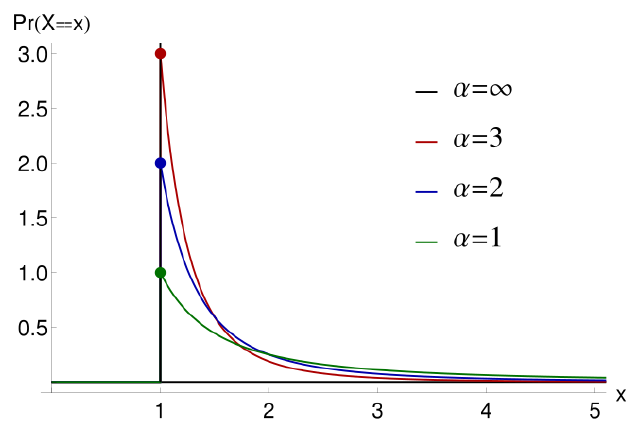
\includegraphics[width=8cm, height=6cm]{pic19}
    \end{center}
    The reason for fitting a pareto distribution for skills at the top is because income distribution is well approximated with a pareto distribution. This suggests that the underlying skill distribution should have a "right pareto tail". If income is pareto distributed with tail index $\alpha_{y}$, then
    \begin{gather*}
        \lim_{y \rightarrow \infty} \frac{1 - Q(y)}{y q(y)} = \frac{1}{\alpha_{y}} \rightarrow \ \text{constant}
    \end{gather*}
    In the data $\frac{1 - Q(y)}{y q(y)}$ is extremely stable at the top as seen below
    \newline
    \begin{center}
    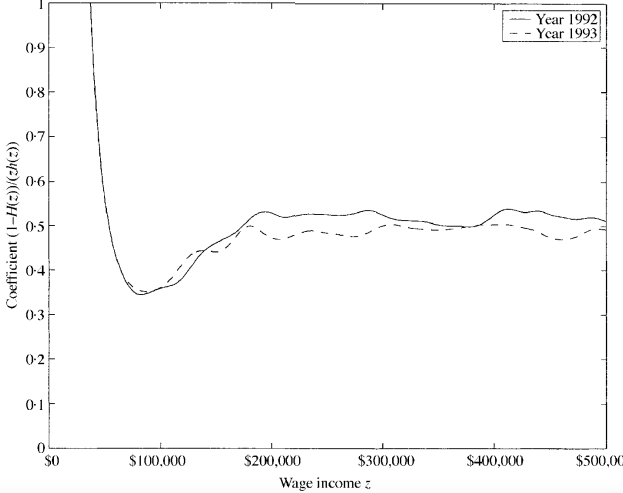
\includegraphics[width=8cm, height=6cm]{pic20}
    \end{center}
    In summary, if the skill distribution is also pareto at the top then
    \begin{gather*}
        \lim_{\theta \rightarrow \infty} \frac{1 - F(\theta)}{\theta f(\theta)} = \frac{1}{\alpha}
    \end{gather*}
    where $\alpha$ is backed out from $\alpha_{y}$ based on $a = (1 + \varepsilon) \alpha_{y}$ (this can be proven by manipulating the FOC of the agent's problem in decentralisation facing the linear top tax rate $\overline{\tau}$)
\end{itemize}
\vspace{2.5mm}
\par \underline{Simulation of Optimal Taxes}: from simulating the model we can derive optimal taxes as being
\newline
\begin{center}
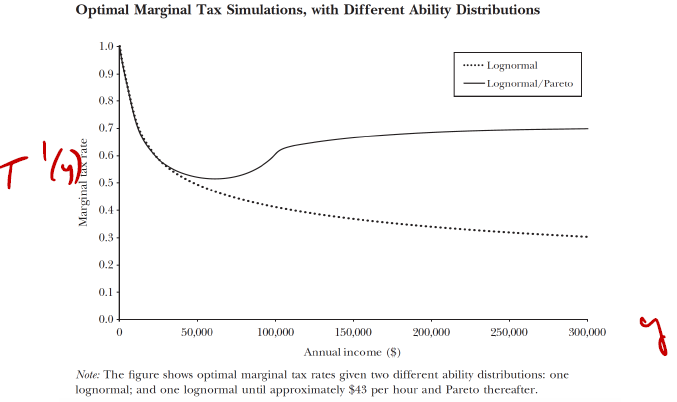
\includegraphics[width=8cm, height=6cm]{pic21}
\end{center}
\begin{itemize}
 \item  \underline{Bottom and Top Distribution Results}: we have that the optimal $T^{'}$ at the bottom is very high, which deters high incomes from not working at full potential (counterpart of the $T^{'}(\theta_{L}) > 0$ result in the two-type model). Moreover, $\frac{1 - F(\theta)}{\theta f(\theta)}$ is very high at the bottom since (1) there are too many individual above the bottom making the numerator big, (2) the denominator being small because of few individual around the bottom and low $\theta$. Due to the low number of individuals and low skill level, distortions induced by high $T^{'}$ for low income agents are not too large
 \item  \underline{Distribution Shape Results}: the optimal $T^{'}$ is U-shaped, mirroring the behaviour of ratio  $\frac{1 - F(\theta)}{\theta f(\theta)}$. $T^{'}$ only becomes progressive at high incomes
 \item  \underline{Qualitative Results}: top tax rates can be quite large for high incomes. The 'zero taxation at the top' (see two type model) only applies to the very top income earner. With an unbounded skill distribution the level of top earnings is not known in advance. Hence, the 'zero taxation at the top' (and the implication that $T^{'}$ decreases at the top) has little empirical and policy relevance
\end{itemize}
\vspace{2.5mm}
\par \underline{Top Tax Formula}: with our optimal tax formula $\frac{T^{*'}(\theta)}{1 - T^{*'}(\theta)} = (1 + \frac{1}{\varepsilon}) (1 - \frac{D(\theta)}{D(\theta_{LB})}) \frac{1 - F(\theta)}{\theta f(\theta)}$, as $\theta \rightarrow \infty$ we have that $D(\theta) \rightarrow 0$ and $\frac{1 - F(\theta)}{\theta f(\theta)} \rightarrow \frac{1}{\alpha}$. Therefore, the optimal asymptotic top tax rate, known as the Diamond-Saez Top Tax Formula, is:
\begin{gather*}
    \overline{T}^{*'} = \frac{1}{1 + \alpha \tfrac{\varepsilon}{1 + \varepsilon}}
\end{gather*}
\begin{itemize}
    \item   \underline{Implications}: with low $\varepsilon$ we have low distortions as $\overline{T}^{*'}$ increases. With low $\alpha$ we have thick right tails of skill distribution and therefore if $\overline{T}^{*'}$ increases few will be affected at the margin but many inframarginally
    \item  \underline{Data}: $\overline{T}^{*'}$ is a key policy instrument to achieve redistribution and accounts for a significant fraction of individual tax revenue (about 40 $\%$ in the US). Using a back-of-the-envelope calibration we have $\varepsilon = 0.25$ as a midrange estimate, $\alpha_{y} = 1.5 \ \rightarrow \ \alpha = 1.88$. This implies that $\overline{T}^{*'} = 73 \% 73$.
    \newline
    Using a sensitivity analysis we have that:
    \newline
    \begin{center}
    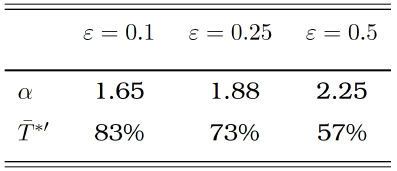
\includegraphics[width=4cm, height=2cm]{pic22}
    \end{center}
    which compares to the following statutory rates across time:
    \newline
    \begin{center}
    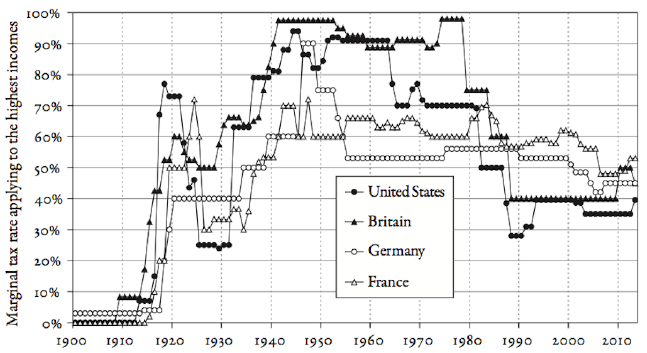
\includegraphics[width=10cm, height=8cm]{pic23}
    \end{center}
\end{itemize}

\newpage

\section{Optimal Dynamic Taxation}
\vspace{2.5mm}
\par \underline{Dynamic Mirrlees Approach}: extends the traditional mirrlees model to a dynamic one involving information friction that endogenise feasible tax instruments, a heterogeneous agents framework, and taxes on capital income
\underline{Baseline Model}: involves a discrete time economy lasting for $T \leq \infty$ periods and an economy populated by a continuum of ex-ante identical individuals
\begin{itemize}
    \item  \underline{Expected Lifetime Utility}: the expected lifetime utility of individuals is
    \begin{gather*}
        U_{0} \equiv \mathbb{E}_{0} \sum_{t-1}^{T} \beta^{t-1} (u(c_{t}) - v(n_{t}))
    \end{gather*}
    where $\beta \in (0,1)$, $c_{t} \geq 0$ is consumption, $n_{t} \geq 0$ is effort, $v$ is strictly increasing and convex, $u$ is strictly increasing and concave (we drop the quasilinearity assumption)
    \item  \underline{Skill}: individuals are heterogeneous with respect to skills/labour productivity where the skill of an agent at time $t$ is given by $\theta_{t} \in \Theta \in \mathbb{R}_{+}$.  \\ Skill shocks are stochastic where $\theta^{t} =  (\theta_{1}, \dots, \theta_{t}) \in \Theta^{t}$ is the history of shocks up to $t$, $\pi_{t} (\theta^{t})$ is the probability of history $\theta^{t}$, and individuals learn their $\theta_{t}$ at the beginning of $t$ with future realizations unknown. \\ the set of skill shocks is discrete where $$\Theta = \left\{ \overline{\theta}_{1}, \overline{\theta}_{2}, \dots, \overline{\theta}_{N} \right\}$$ with $\overline{\theta}_{1} > \overline{\theta}_{2} > \dots > \overline{\theta}_{N}$. \\ Skill shocks are iid such that: $$\pi_{t}(\theta_{t} |\theta^{t-1}) = \pi(\theta_{t})$$, therefore previous history of skill shocks is not going to impact the probability of experience a skill shock of size $\theta_{t}$ and without loss of generality we assume $\mathbb{E}[\theta] = \sum_{\theta \in \Theta}  \pi (\theta) \theta = 1$
    \item  \underline{Agent Output and Borrowing} Agents produce output at period $t$ according to $$y_{t} = \theta_{t} \cdot n_{t}$$ where $\theta_{t}$ and $n_{t}$ are private informations. Agents can borrow and lend at an exogenous gross $R$
    \item  \underline{Firm}: a representative firm produces output by operating a linear technology $$F(Y_{t}, K_{t}) = Y_{t} + RK_{t}$$ where $Y_{t} \equiv \sum_{\theta^{t}} \pi(\theta^{t}) \cdot y(\theta^{t})$ is aggregate effective effort and $K_{t}$ is aggregate savings
    \item  \underline{Aloocation}: an allocation $\left\{ c, y \right\}$ is a sequence of $\left\{ c_{t}, y_{t} \right\}_{t=0}^{T}$ with $(c_{t}, y_{t}): \Theta^{t} \rightarrow \mathbb{R}_{+}^{2}$. An allocation $\left\{ c, y \right\}$ is feasible if and only if
    \begin{gather*}
        \underbrace{\sum_{t=1}^{T} \sum_{\theta^{t} \in \Theta^{T}} R^{1-t} \pi (\theta^{t}) c_{t} (\theta^{t})}_{PV Consumption} \leq \underbrace{\sum_{t=1}^{T} \sum_{\theta^{t} \in \Theta^{t}} R^{1-t} \pi (\theta^{t}) y_{t}(\theta^{t})}_{PV Output}
    \end{gather*}
    \item  \underline{Social Welfare}: assume that a social planner evaluates $\left\{ c, y \right\}$ according to a utilitarian social welfare function that maximizes the expected utility of the agents
    \begin{gather*}
        SWF(c, y) = \sum_{t=1}^{T} \sum_{\theta^{t} \in \Theta^{t}} \beta^{t-1} \pi(\theta^{t}) \big(u(c_{t}(\theta^{t})) - v (n_{t} (\theta^{t})) \big)
    \end{gather*}
    i.e. $SWF(c, y) = U_{0}(c,y)$. Here the motive for redistribution from high to low types is captured by the concavity of $u$ and due to no initial heterogeneity the planner's goal is to provide insurance against $\theta_{t}$ shocks
    \item  \underline{Incentive Compatibility}: we define a reporting strategy by $\sigma_{t}: \Theta^{t} \rightarrow \Theta$ and a history of reporting strategies by $\sigma^{t} = (\sigma_{1}, \dots, \sigma_{t})$. Given this, we have the following IC Contraints:
    \begin{gather*}
        \sum_{t=1}^{T} \sum_{\theta^{t} \in \Theta} \beta^{t-1} \pi(\theta^{t}) \bigg(u(c_{t}(\theta^{t})) - v \big(\frac{y_{t}(\theta^{t})}{\theta_{t}} \big) \bigg) \geq \sum_{t=1}^{T} \sum_{\theta^{t} \in \Theta} \beta^{t-1} \pi(\theta^{t}) \bigg(u(c_{t}(\sigma^{t} (\theta^{t}))) - v \big(\frac{y_{t}(\sigma^{t}(\theta^{t}))}{\theta_{t}} \big) \bigg)
    \end{gather*}
    for all $\sigma^{T}$
    \item  \underline{Optimal Tax Design}: with the goal of the government designing a tax transfer system to provide insurance against $\theta_{t}$ shock, let $\mathcal{T}_{t}(\cdot)$ be a tax system so that agents' budget constraints are
    \begin{gather*}
        c_{t} + k_{t+1} \leq y_{t} + Rk_{t} - \mathcal{T}_{t}(\cdot)
    \end{gather*}
    We are seeking a function $\mathcal{T}_{t}^{*}(\cdot)$ that maximises ex-ante welfare $U_{0}$ in a competitive equilibrium. To find $\mathcal{T}_{t}^{*}(\cdot)$ we follow two steps
    \begin{itemize}
        \item  \underline{Step 1}: find the allocations $\left\{ c^{*}, y^{*} \right\}$ that maximize $U_{0}$ subject to informational frictions (applying dynamic contracts tools)
        \item  \underline{Step 2}: back out a $\mathcal{T}_{t}^{*}(\cdot)$ that implements $\left\{ c^{*}, y^{*} \right\}$ as a competitive equilibrium
    \end{itemize}
    One key difference with the static model is that $\mathcal{T}_{t}^{*}(\cdot)$ is generally not unique. For this reason, we focus on characterising the wedges (distortions) derived from the planning problem
    \item  \underline{Planning Problem}: the constrained optimal allocations $\left\{ c^{*}, y^{*} \right\}$ solve
    \begin{gather*}
        \max_{\left\{ c, y \right\} } \mathbb{E}_{0} \bigg[\sum_{t=1}^{T} \beta^{t-1} \big(u(c_{t}(\theta^{t})) - v\big(\frac{y_{t}(\theta^{t})}{\theta^{t}} \big) \big) \bigg] \\
        \text{subject to}
        \mathbb{E}_{0} \bigg[\sum_{t=1}^{T} R^{1-t} \big(c_{t}(\theta^{t}) - y_{t}(\theta^{t}) \big) \bigg] \leq 0 \tag{RC} \\
        \sum_{t=1}^{T} \sum_{\theta^{t} \in \Theta} \beta^{t-1} \pi(\theta^{t}) \bigg(u(c_{t}(\theta^{t})) - v \big(\frac{y_{t}(\theta^{t})}{\theta_{t}} \big) \bigg) \geq \sum_{t=1}^{T} \sum_{\theta^{t} \in \Theta} \beta^{t-1} \pi(\theta^{t}) \bigg(u(c_{t}(\sigma^{t} (\theta^{t}))) - v \big(\frac{y_{t}(\sigma^{t}(\theta^{t}))}{\theta_{t}} \big) \bigg) \ \forall \ \sigma^{T} \tag(IC)
    \end{gather*}
\end{itemize}
\vspace{2.5mm}
\par \underline{Two Period Model}: focusing on a two period model ($T = 2$) with constant type across time ($\theta_{1} = \theta_{2}$) and two possible types $\Theta = \left\{ \theta_{L}, \theta_{H} \right\}$. We have ex-ante utility:
\begin{gather*}
    U_{0} = \mathbb{E}_{0}\bigg[u(c_{1}) - v(\frac{y_{1}}{\theta}) + \beta \big(u(c_{2}) - v(\frac{y_{2}}{\theta}) \big) \bigg]
\end{gather*}
We have the following resource constraints:
\begin{gather*}
    \sum_{\theta} \pi (\theta) [c_{1} (\theta) - y_{1}(\theta)] + K_{2} = 0 \tag{1} \\
    \sum_{\theta} \pi (\theta) [c_{2} (\theta) - y_{2}(\theta)] = RK_{2} \tag{2}
\end{gather*}
Combining (1) and (2) yields:
\begin{gather*}
\sum_{\theta} \pi (\theta) \bigg[c_{1}(\theta) - y_{1}(\theta) + \frac{1}{R} (c_{2}(\theta) - y_{2}(\theta)) \bigg]
\end{gather*}
Overall, we have the following planning problem:
\begin{gather*}
    \max_{\left\{ c, y \right\}} \sum_{\theta} \pi(\theta) \bigg[u(c_{1}) - v(\frac{y_{1}}{\theta}) + \beta \big(u(c_{2}) - v(\frac{y_{2}}{\theta}) \big) \bigg] \\
    \text{subject to} \\
    \sum_{\theta} \pi (\theta) \bigg[c_{1}(\theta) - y_{1}(\theta) + \frac{1}{R} (c_{2}(\theta) - y_{2}(\theta)) \bigg] \\
    u(c_{1}(\theta)) - v \big(\frac{y_{1} (\theta)}{\theta} \big) + \beta \big(u(c_{2}(\theta)) - v(\frac{y_{2}(\theta)}{\theta}) \big) \geq u(c_{1}(\theta^{'})) - v(\frac{y_{1}(\theta^{'})}{\theta}) + \beta \big(u(c_{2}(\theta^{'})) - v(\frac{y_{2}(\theta^{'})}{\theta}) \big) \ \forall \ \theta, \theta^{'}
\end{gather*}
With ($IC_{H}$) binding at the optimum we transform the planning problem to:
\begin{gather*}
    \max_{\left\{ c, y \right\}} \sum_{\theta} \pi(\theta) \bigg[u(c_{1}) - v(\frac{y_{1}}{\theta}) + \beta \big(u(c_{2}) - v(\frac{y_{2}}{\theta}) \big) \bigg] \\
    \text{subject to} \\
    \sum_{\theta} \pi (\theta) \bigg[c_{1}(\theta) - y_{1}(\theta) + \frac{1}{R} (c_{2}(\theta) - y_{2}(\theta)) \bigg] \\
    u(c_{1}(\theta_{H})) - v \big(\frac{y_{1} (\theta_{H})}{\theta_{H}} \big) + \beta \big(u(c_{2}(\theta_{H})) - v(\frac{y_{2}(\theta_{H})}{\theta_{H}}) \big) \geq u(c_{1}(\theta_{L})) - v(\frac{y_{1}(\theta_{L})}{\theta_{H}}) + \beta \big(u(c_{2}(\theta_{L})) - v(\frac{y_{2}(\theta_{L})}{\theta_{H}}) \tag{$IC_{H}$}
\end{gather*}
\begin{itemize}
    \item  \underline{First Best Allocation}: we have two key conditions for optimality
    \begin{itemize}
        \item  \underline{Tntratemporal Condition}: the intratemporal efficiency condition must hold where $MRS_{l, c} = MRT_{l,c}$ such that
        \begin{gather*}
            \frac{\tfrac{v^{'}(y_{t}^{FB})}{\theta_{t}}}{u^{'}(c_{t}^{FB})} = \theta_{t}
        \end{gather*}
        \begin{itemize}
            \item  \underline{Logic}: if intratemporal efficiency does not hold then I can rearrange $(c, l)$ and increase $U_{0}$
            \item  \underline{Alternative Form}: this can be alternatively written as
            \begin{gather*}
                \underbrace{v^{'}(l_{t}^{FB})}_{\text{Marginal Cost of Y Increase}} = \underbrace{\theta_{t} u^{'}(c_{t}^{FB})}_{\text{Marginal Benefit of Y Increase}}
            \end{gather*}
        \end{itemize}
        \item  \underline{Intertemporal Condition}: the intertemporal efficiency condition must hold where $MRS_{c_{1}, c_{2}} = MRT_{c_{1}, c_{2}}$ such that
        \begin{gather*}
            \frac{u^{'}(c_{1}^{FB})}{\beta u^{'}(c_{2}^{FB})} = R
        \end{gather*}
        \begin{itemize}
            \item  \underline{Alternative Form}: this can be alternatively written as
            \begin{gather*}
                \underbrace{u^{'}(c_{1}^{FB})}_{\text{Marginal Cost of $c_{2}$ Increase}} = \underbrace{R \beta u^{'}(c_{2}^{FB})}_{\text{Marginal Benefit of $c_{2}$ Increase}}
            \end{gather*}
        \end{itemize}
    \end{itemize}
    The constrained optimal allocation also features two types of wedges/distortions. These can be interpreted as implicit marginal taxes and will shape $\mathcal{T}_{t}^{*}(\cdot)$ in the decentralization
    \begin{itemize}
        \item  \underline{Labor Wedge at $t$}: this involves a distortion between $MRS_{l_{t}, c_{t}}$ and $MRT_{l_{t}, c_{t}}$ due to the implicit marginal tax on labor income at $t$. Note that
        \begin{gather*}
            1 - \tau_{t}^{y}(\theta) \equiv \frac{v^{'}(y_{t}^{*}(\theta)/\theta)/theta}{u^{'}(c_{t}^{*}(\theta))}
        \end{gather*}
        We have for a two-period dynamic model with $|\Theta| = 2$ and constant types (i.e. $\theta_{t} = \theta$ for $t = 1,2$) that for all $t$: $\tau_{t}^{y}(\theta_{L}) > 0$ and $\tau_{t}^{y}(\theta_{H}) = 0$
        \item  \underline{Savings Wedge at $t = 1$}: this involves a distortion between $MRS_{c_{1}, c_{2}}$ and $MRT_{c_{1}, c_{2}}$ due to the implicit marginal tax on capital income. Note that
        \begin{gather*}
            1 - \tau^{s}(\theta) \equiv \frac{u^{'}(c_{1}^{*}(\theta))}{\beta R u^{'}(c_{2}^{*}(\theta))}
        \end{gather*}
        We have for a two-period model with $|\Theta| = 2$ and constant types (i.e. $\theta_{t} = \theta$ for $t = 1,2$) that $\tau^{s}(\theta_{L}) = \tau^{s}(\theta_{H}) = 0$
    \end{itemize}
    \item  \underline{Final Planner Problem}: based on the wedges, when types are constant it is optimal not to distort savings decisions - a key assumption of this model. Thus our planning problem becomes:
     \begin{gather*}
         \max_{\left\{ c, y \right\}} \sum_{\theta_{1}, \theta_{2}} \pi (\theta_{1}) \pi (\theta_{2}) \bigg[ u(c_{1}(\theta_{1})) - v(\frac{y_{1} (\theta_{1})}{\theta_{1}}) + \beta \big(u(c_{2}(\theta_{2})) - v(\frac{y_{2}(\theta^{2})}{\theta^{2}}) \big) \bigg] \\
         \text{subject to} \\
         \sum_{\theta_{1}, \theta_{2}} \pi (\theta_{1}) \pi (\theta_{2}) \big[c_{1}(\theta_{1}) - y_{1}(\theta_{1}) + \frac{1}{R} (c_{2}(\theta^{2}) - y_{2}(\theta^{2})) \big] = 0 \\
         u(c_{1}(\theta_{1})) - v(\frac{y_{1}(\theta_{1})}{\theta_{1}}) + \beta \sum_{\theta_{2}} \pi(\theta_{2}) \big(u(c_{2}(\theta^{2})) - v (\frac{y_{2}(\theta^{2})}{\theta^{2}}) \big) \geq u(c_{1}(\sigma_{1}(\theta_{1}))) - v(\frac{y_{1}(\sigma_{1}(\theta_{1}))}{\theta_{1}}) + \beta \sum_{\theta_{2}} \pi(\theta_{2}) \big(u(c_{2}(\sigma^{2}(\theta^{2}))) - v(\frac{y_{2}(sigma^{2}(\theta^{2}))}{\theta^{2}}) \big)
     \end{gather*}
     for all ($\theta_{1}, \sigma_{1}, \theta^{2}, \sigma^{2}$).
     \begin{itemize}
         \item  \underline{Saving Wedge}: the savings wedge with stochastic types is:
         \begin{gather*}
             1 - \tau^{s}(\theta_{1}) \equiv \frac{u^{'}(c_{1}^{*}(\theta_{1}))}{\beta R \mathbb{E}_{1}[u^{'}(c_{2}^{*}(\theta_{1},\theta_{2}))]}
         \end{gather*}
         \item  \underline{Inverse Euler Equation}: consider the two-period model with stochastic types. The constrained efficient allocation satisfies
         \begin{gather*}
             \frac{1}{u^{'}(c_{1}^{*}(\theta_{1}))} = \frac{1}{\beta R} \sum_{\theta_{2}}
         \end{gather*}
         This is essentially a euler equation for the reciprocal of the marginal utilities.
         \begin{itemize}
             \item  \underline{Proof - Variational Approach with Utility Space}: consider the following variation of the optimal solution: fix $\theta$ and let
             \begin{gather*}
                 u_{1}^{\varepsilon}(\theta_{1}) = u_{1}^{*}(\theta_{1}) - \varepsilon, \ \ \varepsilon > 0 \\
                 u_{2}^{\varepsilon}(\theta_{1}, \theta_{2}) = u_{2}^{*} (\theta_{1}, \theta_{2}) + \frac{\varepsilon}{\beta}, \ \ \forall \theta_{2}
             \end{gather*}
             where $u_{1}^{*}(\theta_{1})$ is consumption utility at optimum at $t=1$ and $u_{2}^{*}(\theta_{1}, \theta_{2})$ is consumption utility at optimum at $t=2$. It is easy to show that the perturbed allocation is such that (1) the objective function doesn't change and (2) the ICs are satisfied. Therefore, a necessary condition for the original allocation to be optimal is that resources spent in implementing the allocation are minimized at $\varepsilon = 0$. Let the resource cost of delivering the new allocation be:
             \begin{gather*}
                 \mathcal{L}^{\varepsilon}(\theta_{1}) = \underbrace{u^{-1}(u_{1}^{\varepsilon}(\theta_{1}))}_{c_{1}(\theta_{1})} + \frac{1}{R} \sum_{\theta_{2}} \pi (\theta_{2}) \underbrace{u^{-1}(u_{2}^{\varepsilon}(\theta_{1},\theta_{2}))}_{c_{2}^{\varepsilon}(\theta_{1}, \theta_{2})}
             \end{gather*}
             If $u_{1}^{*}(\theta_{1})$ and $u_{2}^{*}(\theta_{1}, \theta_{2})$ are optimal, we must have that:
             \begin{gather*}
                 \frac{\partial \mathcal{L}^{\varepsilon}(\theta_{1})}{\partial \varepsilon} \big|_{\varepsilon = 0} = 0 \tag{*}
             \end{gather*}
             Note that:
             \begin{gather*}
                 \mathcal{L}^{\varepsilon} (\theta_{1}) = u^{-1}(u_{1}^{*}(\theta_{1}) - \varepsilon) + \frac{1}{R} \sum_{\theta_{2}} \pi (\theta_{2}) u^{-1} (u_{2}^{*}(\theta_{1}, \theta_{2}) + \tfrac{\varepsilon}{\beta})
             \end{gather*}
             Then condition (*) boils down to:
             \begin{gather*}
                 \frac{\partial \mathcal{L}^{\varepsilon}(\theta_{1})}{\partial \varepsilon} \big|_{\varepsilon = 0} = 0 \Leftrightarrow \overbrace{\frac{1}{u^{'}(underbrace{u^{-1}(u_{1}^{*}(\theta_{1}))}_{c_{1}^{*}(\theta_{1})})} = \frac{1}{R \beta} \sum_{\theta_{2}} \pi(\theta_{2}) \frac{1}{u^{'}(\underbrace{ u^{-1} (u_{2}^{*}(\theta_{1}, \theta_{2})) }_{c_{2}^{*}(\theta_{1},\theta_{2})})} }^{\text{IEE}}
             \end{gather*}
             Use that: $[F^{-1}]^{'}(x) = \frac{1}{f^{'}(f^{-1}(x))}$
         \end{itemize}
         \item  \underline{Savings Taxes}: for the two period model with stochastic types, suppose that for some $\theta_{1}, c_{2}^{*}(\theta_{1}, \theta_{2})$ is not independent of $\theta_{2}$. Then we have that
         \begin{gather*}
             \tau^{s}(\theta_{1}) > 0, \ \ \forall \theta_{1}
         \end{gather*}
         \begin{itemize}
             \item  \underline{Proof}: by the inverse Euler Equation we have that
             \begin{gather*}
                 \frac{1}{u^{'}(c_{1}^{*}(\theta_{1}))} = \frac{1}{R \beta} \mathbb{E}_{1} \big[\frac{1}{u^{'}(c_{2}^{*}(\theta_{1}, \theta_{2}))} \big]
             \end{gather*}
             Applying Jensen's inequality we have:
             \begin{gather*}
                 \frac{1}{u^{'}(c_{1}^{*}(\theta_{1}))} \geq \frac{1}{R \beta \mathbb{E}_{1}[u^{'}(c_{2}^{*}(\theta_{1}, \theta_{2}))]} \Leftrightarrow 1 \geq \frac{u^{'}(c_{1}^{*})}{\beta R u^{'}(c_{2}^{*})}
             \end{gather*}
             If $c_{2}^{*}(\theta_{1}, \theta^{2})$ is not independent of $\theta_{2}$ then the inequality is strict. Using this into the definition of $\tau^{s}(\theta_{1})$ proves the result
             \item  \underline{Jensen's Inequality}: $E[\frac{1}{x}] \geq \frac{1}{E[x]}$
             \item  \underline{Intuition behind $\tau^{s}(\theta_{1}) > 0$}: with stochastic types, incentives to exert high effort should also be provided in period $t=2$. When agents save, providing such inventives is more costly since higher savings creates a positive income effect which leads to reducing effort. This goes against the Ramsey approach, where taxing capital/savings is never optimal in the long run, and the Atkinson-Stiglitz result, where taxing capital/savings is never optimal in the presence of non-linear labour income taxes
         \end{itemize}
         \item  \underline{Implementing the Savings Wedge}: in an implementation with income taxes, consumers face the following budget constraints
         \begin{align*}
             c_{1} + k_{2} &\leq y_{1} - T_{1}(y_{1}) \\
             c_{2} &\leq y_{2} + R k_{2} - T_{2}(y_{1}, y_{2}, R k_{2})
         \end{align*}
         Since tax implementations in the dynamic model are non-unique, different specifications for $T_{2}$ could implement the savings wedge $\tau^{s}$
     \end{itemize}
\end{itemize}
\vspace{2.5mm}
\par \underline{Finite Horizon Model}: in the finite horizon version of the dynamic mirrlees model we have the following planning problem:
\begin{gather*}
    \max_{c,y} \mathbb{E}_{0} \bigg[\sum_{t=1}^{T} \beta^{t-1} \big(u(c_{t}(\theta^{t})) - v(\frac{y_{t}(\theta^{t})}{\theta_{t}}) \big) \bigg] \\
    \text{subject to} \\
    \mathbb{E}_{0} \big[\sum_{t=1}^{T} R^{1-t} (c_{t}(\theta^{t}) - y_{t}(\theta^{t})) \big] \leq 0 \\
    \mathbb{E}_{0} \big[\sum_{t=1}^{T} \beta^{t-1} (u(c_{t}(\theta^{t})) - v(\frac{y_{t} (\theta^{t})}{\theta})) \big] \geq \mathbb{E}_{0} \big[\sum_{t=1}^{T} \beta^{t-1} (u(c_{t}(\sigma^{t}(\theta^{t}))) - v(\frac{y_{t} (\sigma^{t}(\theta^{t})}{\theta})) \big] \ \ \forall \sigma^{t}
\end{gather*}
Given history $\theta^{t-1}$, we define continution utility from reporting $\theta$ at $t$ and reporting truthfully from $t+1$ onwards by:
\begin{gather*}
    w_{t}(\theta^{t-1}, \theta) = \sum_{s=1}^{T-1}\sum_{\theta^{t+s}} \beta^{s-1} \pi(\theta^{t+s}) \big[ u(c_{t+s}(\theta^{t-1},\theta,\theta_{t+1}^{t+s})) - v(\frac{y_{t+s}(\theta^{t-1}, \theta, \theta^{t+1}_{t+1})}{\theta_{t+s}}) \big]
\end{gather*}
It can be shown that the original set of ICs is equivalent to:
\begin{gather*}
    u(c_{t}(\theta^{t-1}, \theta)) - v(\frac{y_{t}(\theta^{t-1},\theta)}{\theta}) + \beta w_{t}(\theta^{t-1},\theta) \geq u(c_{t}(\theta^{t-1}, \widehat{\theta})) - v(\frac{y_{t}(\theta^{t-1},\widehat{\theta})}{\theta}) + \beta w_{t}(\theta^{t-1}, \widehat{\theta})
\end{gather*}
for all $t, \theta^{t-1}, \theta, \widehat{\theta}$. Therefore, the planning problem now becomes:
\begin{gather*}
    \max_{c,y} \mathbb{E}_{0} \bigg[\sum_{t=1}^{T} \beta^{t-1} \big(u(c_{t}(\theta^{t})) - v(\frac{y_{t}(\theta^{t})}{\theta_{t}}) \big) \bigg] \\
    \text{subject to} \\
    \mathbb{E}_{0} \big[\sum_{t=1}^{T} R^{1-t} (c_{t}(\theta^{t}) - y_{t}(\theta^{t})) \big] \leq 0 \\
    u(c_{t}(\theta^{t-1}, \theta)) - v(\frac{y_{t}(\theta^{t-1},\theta)}{\theta}) + \beta w_{t}(\theta^{t-1},\theta) \geq u(c_{t}(\theta^{t-1}, \widehat{\theta})) - v(\frac{y_{t}(\theta^{t-1},\widehat{\theta})}{\theta}) + \beta w_{t}(\theta^{t-1}, \widehat{\theta}) \\
    w_{t}(\theta^{t}) = sum_{\theta} \pi(\theta) \big[u(c_{t+1}(\theta^{t}, \theta)) - v(\frac{y_{t+1}(\theta^{t}, \theta)}{\theta}) + \beta w_{t+1}(\theta^{t}, \theta) \big]
\end{gather*}
for all $t, \theta^{t-1}, \theta, \widehat{\theta}$. Since this problem has no recursive structure we can transofrm it to the dual problem of cost minimization given $w_{0}$:
\begin{gather*}
    \max_{c,y} - \mathbb{E}_{0} \big[\sum_{t=1}^{T} R^{1-t} (c_{t}(\theta^{t}) - y_{t}(\theta^{t})) \big]
    \text{subject to} \\
    u(c_{t}(\theta^{t-1}, \theta)) - v(\frac{y_{t}(\theta^{t-1},\theta)}{\theta}) + \beta w_{t}(\theta^{t-1},\theta) \geq u(c_{t}(\theta^{t-1}, \widehat{\theta})) - v(\frac{y_{t}(\theta^{t-1},\widehat{\theta})}{\theta}) + \beta w_{t}(\theta^{t-1}, \widehat{\theta}) \\
    w_{t}(\theta^{t}) = sum_{\theta} \pi(\theta) \big[u(c_{t+1}(\theta^{t}, \theta)) - v(\frac{y_{t+1}(\theta^{t}, \theta)}{\theta}) + \beta w_{t+1}(\theta^{t}, \theta) \big]
\end{gather*}
for all $t, \theta^{t-1}, \theta, \widehat{\theta}$. Thereby, we solve this problem by minimizing the cost of delivering $w_{0}$. This dual problem admits a nice recursive formulation:
\begin{gather*}
    K_{t}(x) = \max_{c(\theta), y(\theta), w(\theta)} \sum_{\theta} \pi(\theta) [y(\theta) - c(\theta) + R^{-1}K_{t+1}(w(\theta))] \\
    \text{subject to} \\
    x = \sum_{\theta} \pi (\theta) \big[ u(c(\theta)) - v(\frac{y(\theta)}{\theta}) + \beta w(\theta) \big] \tag{PKC} \\
    u(c(\theta)) - v(\frac{y(\theta)}{\theta}) + \beta w (\theta) \geq u(c(\widetilde{\theta})) - v(\frac{y(\widetilde{\theta})}{\theta}) + \beta w(\widetilde{\theta}), \ \ \forall (\theta, \widetilde{\theta}) \tag{IC}
\end{gather*}
\vspace{2.5mm}
\par \underline{Infinite Horizon}: extending the framework to $T = \infty$ we have
\begin{gather*}
    K(x) = \max_{c(\theta), y(\theta), w(\theta)} \sum_{\theta} \pi (\theta) [y(\theta) - c(\theta) + R^{-1} K (w(\theta))] \\
    \text{subject to} \\
    x = \sum_{\theta} \pi (\theta) \big[u(c(\theta)) - v(\frac{y(\theta)}{\theta}) + \beta w(\theta) \big] \tag{PKC} \\
    u(c(\theta)) - v(\frac{y(\theta)}{\theta}) + \beta w(\theta) \geq u(c(\widetilde{\theta})) - v(\frac{y(\widetilde{\theta})}{\theta}) +  \beta w(\widetilde{\theta}), \ \ \forall (\theta, \widetilde{\theta}) \tag{IC}
\end{gather*}
Note that technical conditions should also be met such that solutions to the original problem and recursive formulation coincide. The key results of the two period model extend to the infinite horizon model, partiicularly the positive savings wedge and implementations discussed. We set $R = \beta^{-1}$ since this is the only configuration consistent with a steady state and otherwise aggregate consumption would not be constant across periods
\begin{itemize}
    \item  \underline{Inequality Dynamics}: consider the special case with two types: $$\Theta = \left\{ \theta_{L}, \theta_{H} \right\}$$ The ICs for this problem are
    \begin{gather*}
        u(c(\theta_{H})) - v(\frac{y(\theta_{H})}{\theta_{H}}) + \beta w(\theta_{H}) \geq u(c(\theta_{L})) - v(\frac{y(\theta_{L})}{\theta_{H}}) + \beta w(\theta_{L}) \\
        u(c(\theta_{L})) - v(\frac{y(\theta_{L})}{\theta_{L}}) + \beta w(\theta_{L}) \geq u(c(\theta_{H})) = v(\frac{y(\theta_{H})}{\theta_{L}}) + \beta w(\theta_{H})
    \end{gather*}
    Using that only ($IC_{H}$) is binding at the optimum we can show that at an interior solution
    \begin{gather*}
        y(\theta_{H}) \geq y(\theta_{L}), \ c(\theta_{H}) \geq c(\theta_{L}), \ w(\theta_{H}) \geq w(\theta_{L})
    \end{gather*}
    Here $w$ serves as a new margin for incentive provision where to provide incentives the planner spreads out continuation utilities. Hence, providing incentives to reveal private information leads to inequality in lifetime utility promises and consumption. To analyse the optimal degree of inequality, let $\Psi_{t}$ be the distribution of promised utilities at $t$. The optimal contract defines a mapping $\Omega$ such that
    \begin{gather*}
        \Psi_{t+1} = \Omega (\Psi_{t})
    \end{gather*}
    with $\Psi_{0}$ given. This gives us the law of motion for $\Psi_{t}$. The aim then is to find the steady state distribution of $\Psi^{*}$ subject to $\Psi^{*} = \Omega (\Psi^{*})$. Rearranging the planning problem's first order conditions reveals that the optimal contract is such that
    \begin{gather*}
        K^{'}(x) = \mathbb{E} [K^{'} (w(\theta))]
    \end{gather*}
    This implies that $\left\{ K^{'}(w_{t}(\theta^{t})) \right\}$ is martingale and therefore has the following convergence property:
    \begin{gather*}
        x_{t} \rightarrow RV \\
        E_{t}[x_{t+1}] = x_{t} \rightarrow \ \text{martingale property}
    \end{gather*}
    \item  \underline{Immiseration Result}: suppose consumption utility $u$ is unbounded below. Then
    \begin{gather*}
        w_{t}(\theta^{t}) \rightarrow - \infty
    \end{gather*}
    as $t \rightarrow \infty$ with probability 1. Since this implies that $c_{t} \rightarrow 0$, in the long run almost everyone is trapped at misery. Note that this does not mean everyone's consumption converges to zero, there will still be some agents with strictly positive consumption but their measure vanishes at $t \rightarrow \infty$. In other words, inequality grows without bounds over time and a measure 0 of individuals consume the entire production.
    \begin{itemize}
        \item  \underline{Proof}: important properties of the value function K are that: K is continuous, strictly concave, strictly decreasing, differentiable, that $\lim_{w \rightarrow - \infty} K(w) = \lim_{w \rightarrow -\infty}K^{'}(w) = 0$ and $\lim_{w \rightarrow \overline{w}} K(w) = \lim_{w \rightarrow \overline{w}}K^{'}(w) = \infty$.
        \newline
        \begin{center}
            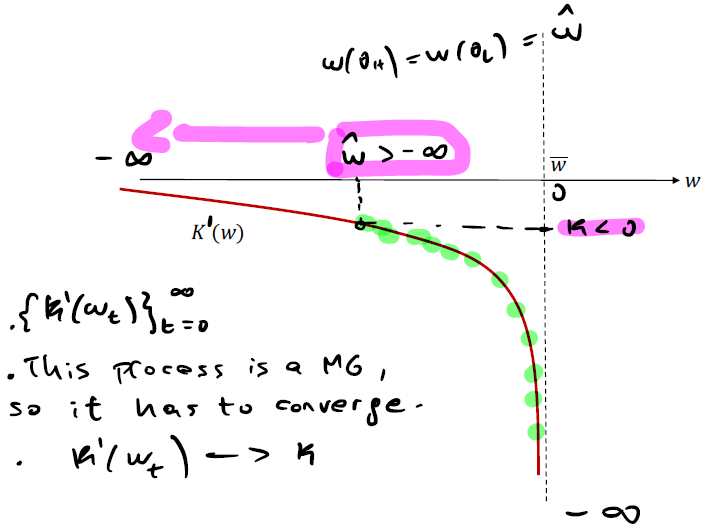
\includegraphics[width=8cm, height=6cm]{pic25}
        \end{center}
        For being a MG, $K^{'}(w_{t})$ converges to a random variable with probability 1. It is easy to see that $K^{'}(w_{t})$ must converge to 0 since suppose that $K^{'}(w_{t}) \rightarrow k \leq 0$ (recall that K is decreasing) then $w_{t} \rightarrow \widehat{w} > - \infty$, where $\widetilde{w}$ is defined by $K^{'}(\widetilde{w}) = k$. This implies that, in the limit, continuation utilities are not spread out and so $w(\theta_{L}) = w(\theta_{H})$ which is a contradition. Hence, $K^{'}(w_{t})$ must converge to 0 so that $w_{t} \rightarrow - \infty$
        \item  \underline{Intuition}: providing incentives is cheaper if the planner introduces a downward drift on consumption becaue utility is concave. Therefore, for poor individuals, even tiny increments in consumption would make them super happy.
        \item  \underline{Issue}: immersiration is an issue and there is no well-defined answer regarding the optimal level of inequality ($\Psi^{*}$ does not exist)
        \item  \underline{Solving for $\Psi^{*}$}: many economists have provided restricted solutions for if we suppose that $\Psi^{*}$ exists
        \begin{itemize}
            \item  \underline{Lower Bound}: impose an exogenous lower bound on continuation utility $\underline{w} > -\infty$
            \item  \underline{Commitment}: impose lack of commitment by the planner
            \item  \underline{Philosophical Arguments}: impose political economy arguments to microfound $\underline{w} > - \infty$
            \item  \underline{Discounting}: impose that the social discount factor < private discount factor
        \end{itemize}
    \end{itemize}
\end{itemize}

\newpage
\section{Optimal Unemployment Insurance}
\vspace{2.5mm}
\par \underline{Model}: economy lasts for $T = \infty$ periods, populated by a worker (agent) and an unemployment insurance agency (principal). The worker can be employed or unemployed and the goal is to characterise the optimal unemployment insurance contract between an unemployment agency and a worker
\begin{itemize}
    \item  \underline{Worker's Preferences}
    \begin{gather*}
        U = \mathbb{E}_{0} \sum_{t=0}^{\infty} \beta^{t} [u(c_{t}) - a_{t}]
    \end{gather*}
    where $c_{t} \geq 0$ is consumption, $u(\cdot)$ is strictly increasing, strictly concave, and bounded below, and $a_{t} \geq 0$ is search effort that determines the probability of finding a job at $t+1$
    \item  \underline{Employment}: employment is an absorbing state (one spell model) where all jobs are alike and pay wage $w > 0$ forever and the search effort is $a = 0$ if employed
    \item  \underline{Unemployment}: while unemployed the worker finds a job with probability $p(a)$ where $p^{'}(a) > 0, p^{''}(a) < 0, p(0) = 0$. During this time, the worker receives unemployment beneftis from the insurance agency
    \begin{itemize}
        \item  \underline{Non-Storable Consumption Good}: the worker cannnot save or borrow. Unemployment benefits are the only source of consumption ($c_{t}$) during unemployment
    \end{itemize}
    \item  \underline{Private Information Friction}: $a_{t}$ is unobservable by the insurance agency, with the information friction coming from private action ($a$) rather than private types (making this a moral hazard rather than adverse selection problem)
    \begin{itemize}
        \item  \underline{Note}: though this is a moral hazard instead of adverse selection problem, similar techniques (such as the Revelation Principle) still hold
    \end{itemize}
    \item  \underline{Value of Employment $V^{e}$}: let $V^{e}$ be the value of being employed for the worker. We assume that once a worker finds a job, she is beyond the reach of the agency (i.e. no further obligations such as taxes based on unemployment length). Given that jobs are permanent and pay $w$ forever, we have
    \begin{gather*}
        V^{e} = \frac{u(w)}{1 - \beta}
    \end{gather*}
    \item  \underline{Value of Autarky $V_{aut}$}: let $V_{aut}$ denote the value of being unemployed and not having acccess to unemployment insurance. $V_{aut}$ is the solution to the Bellman Equation:
    \begin{gather*}
        V_{aut} = \max_{a} \left\{ u(0) - a + \beta [p(a)V^{e} + (1-p(a)) V_{aut}] \right\}
    \end{gather*}
\end{itemize}
\vspace{2.5mm}
\par \underline{Model with Full Information}: suppose the UI agency can observe and control $c$ and $a$. The agency designs a UI contract to give the unemployed worker expected utility $V \geq V_{aut}$. Let $C(V)$ be the expected discounted cost of delivering $V \geq V_{aut}$, the Bellman Equation therefore becomes:
\begin{gather*}
    C(V) = \min_{c,a,V^{u}} \left\{ c + \beta (1 - p(a)) C(V^{u}) \right\} \\
    \text{subject to} \\
    u(c) - a + \beta \left\{p(a)V^{e} + (1 - p(a)) V^{u} \right\} = V \tag{PKC}
\end{gather*}
Note that PKC is the promise keeping constraint, we assume the agency discounts future payoffs using $\beta$, c is the unemployment benefit, C is structky convex, and $V \geq V_{aut}, V^{u} \geq V_{aut}$. Let $\lambda > 0$ be the multiplier on the (PKC).
\begin{itemize}
    \item  \underline{Solution}: the first order conditions are:
    \begin{align*}
        \frac{\partial}{\partial c} = 0 &\rightarrow \frac{1}{u^{'}(c)} = \lambda \tag{1} \\
        \frac{\partial}{\partial a} = 0 &\rightarrow C(V^{u}) = \lambda \big[\frac{1}{\beta p^{'}(a)} - (V_{e} - V^{u}) \big] \geq 0 \tag{2} \\
        \frac{\partial}{\partial V^{u}} = 0 &\rightarrow C^{'}(v^{u}) = \lambda \\
        \text{Envelope Theorem} \ &\rightarrow \ C^{'}(V) = \lambda
    \end{align*}
    By FOC (3) and (4) we have that $V^{u} = V$ using that C is convex. In sequential notation this is:
    \begin{gather*}
        V_{t+1} = V_{t} \ \ \forall t
    \end{gather*}
    Unemployment benefits can be written as:
    \begin{gather*}
        C_{t} = c(V_{t}) \rightarrow c_{t} = c_{t+1} \ \forall t \\
        a_{t} = a(V_{t}) \rightarrow a_{t} = a_{t+1} \ \forall t
    \end{gather*}
    Rearranging the optimality conditions we get the following proposition: \textit{Under full information, c and a are held constant during the unemployment state}. In the absence of private information, unemployment benefits (c) are fully smoothed during the unemployment state. This implies that the replacement ratio $c/w$ is also constant
    \item  \underline{Private Information Issue}: the full information solution is not achievable under private information. Note that by FOC (2), the socially optimal level of effort under full information $a^{*}$ satisfies:
    \begin{gather*}
        [\beta p^{'}(a^{*})]^{-1} > V^{e} - V^{u*}
    \end{gather*}
    However, if offered ($c^{*}, v^{u*}$) the worker could choose $a$ according to:
    \begin{gather*}
        a^{private} \in \arg \max_{a} \left\{ u(c^{*}) - a + \beta [p(a)V^{e} + (1-p(a))V^{u*}] \right\}
    \end{gather*}
    This leads to:
    \begin{gather*}
        [\beta p^{'} (a^{private})]^{-1} = V^{e} - V^{u*}
    \end{gather*}
    Since $p$ is concave we have that $a^{*} > a^{private}$. This is as the worker does not take into account the cost of the UI scheme and therefore chooses a level of effort below the socially optimal one.
\end{itemize}
\vspace{2.5mm}
\par \underline{Model with Asymmetric Information}: as effort is not observed, we must ensure that the agent optimally chooses the level of effort $a$ prescribed by the contract. Therefore, we have that:
\begin{gather*}
    a \in \arg \max_{\widehat{a}} \left\{ u(c) - \widehat{a} + \beta [p(\widehat{a})V^{e} + (1-p(\widehat{a}))V^{u}] \right\}
\end{gather*}
The necessary and sufficient condition is that $a$ satisfies
\begin{gather*}
    \beta p^{'}(a) (V^{e} - V^{u}) = 1
\end{gather*}
Note that the optimal level of effort is $a > 0$ if and only if $V^{e} - V^{u}$. Therefore, we have the following planning problem:
\begin{gather*}
    C(V) = \min_{c, a, V^{u}} \left\{ c + \beta (1 - p(a)) C(V^{u}) \right\} \\
    \text{subject to} \\
    u(c) - a + \beta \left\{ p(a)V^{e} + (1 - p(a))V^{u} \right\} = V \tag{PKC} \\
    \beta p^{'}(a) (V^{e} - V^{u}) = 1 \tag{IC}
\end{gather*}
Where we assume that $C(V)$ is strictly convex.
\begin{itemize}
    \item  \underline{Solution}: let $\lambda > 0$ be the multiplier on the (PKC) and $\mu$ be the multiplier on the (IC). We have the following first order conditions:
    \begin{align*}
        \frac{\partial}{\partial c} = 0 &\rightarrow \frac{1}{u^{'}(c)} = \lambda \tag{1} \\
        \frac{\partial}{\partial a} = 0 &\rightarrow C(v^{u}) = -\mu \frac{p^{''}(a)}{p^{'}(a)} (V^{e} - V^{u}) \\
        \frac{\partial}{\partial V^{u}} = 0 &\rightarrow C^{'}(V^{u}) = \lambda - \mu \frac{p^{'}(a)}{1 - p(a)}
    \end{align*}
    Rearranging the first order conditions we get the proposition: \textit{under private information - (1) unemployment benefits decrease with the duration of unemployment, (2) search effort rises with the duration of unemployment}.
    The planner knows that $p^{'}(a) > 0$. Exploiting $p^{'}(a) > 0$, the principal introduces duration dependence to provide incentives to search. Using the 'carrot' we will have high beenfits and low effort early in the unemployment spell. Using the 'stick' we will have low benefits and high effort later in the spell.
    \item  \underline{Numerical Example}: $\beta = 0.99$ with a weekly frequency, $u(c) = \frac{c^{1-\sigma}}{1 - \sigma}$, $\sigma = 0.5$, $p(a) = 1 - \exp(-ra)$ with $r = 3 \times 10^{-1}$, $w = 100$
    \newline
    \begin{center}
        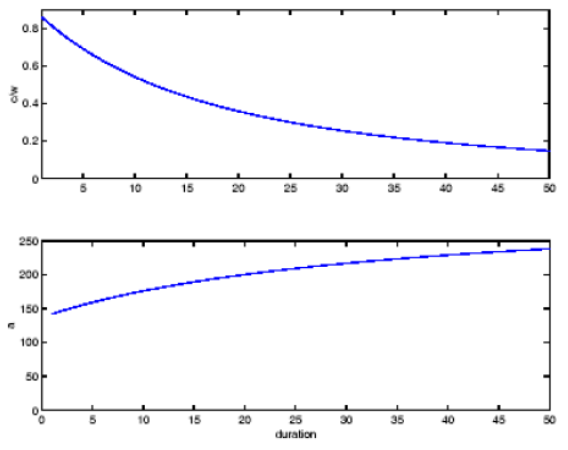
\includegraphics[width=8cm, height=6cm]{pic26}
    \end{center}
    \item  \underline{Model vs. Data}: in most OECD countries, unemployment benefits decrease with the duration of Unemployment
    \newline
    \begin{center}
        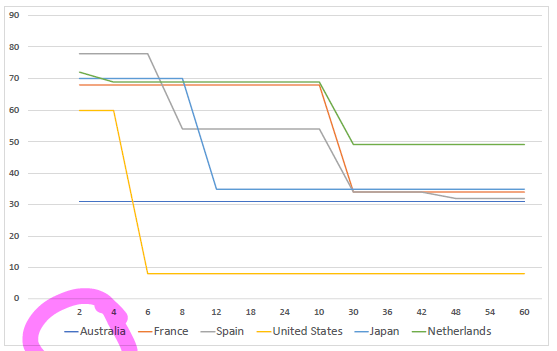
\includegraphics[width=8cm, height=6cm]{pic27}
    \end{center}
\end{itemize}
\vspace{2.5mm}
\par \underline{Model with Employment Taxes}: if we allow the unemployment agency to tax workers once employed we have the key result that taxes typically increase with the duration of the unemployment spell and that the cost savings from switching to this scheme can be large. We have the same environment as before but now the UI agency can use a permanent tax on labor income $\tau$
\begin{itemize}
    \item  \underline{Value of Employment}: this is now:
    \begin{gather*}
        V^{e} = \frac{u(w - \tau)}{1 - \beta}
    \end{gather*}
    We use $V^{e}$ instead of $\tau$ as the control variable for convenience. Therefore, we write tax as a function of $V^{e}$ as:
    \begin{gather*}
        \tau = w - u^{-1}((1-\beta)V^{e})
    \end{gather*}
    \item  \underline{Continuation Cost}: for the agency in the event of employment::
    \begin{gather*}
        W(V^{e}) = \frac{-w + u^{-1}((1-\beta)V^{e})}{1 - \beta}
    \end{gather*}
    \item  \underline{Planning Problem}: this becomes:
    \begin{gather*}
        C(V) = \min_{c,a,V^{u},V^{e}} \left\{ c + \beta (1- p(a)) C(V^{u}) + \beta p(a)W(V^{e}) \right\} \\
        \text{subect to} \\
        u(c) - a + \beta \left\{ (1 - p(a))V^{u} + p(a)V^{e} \right\} = V \tag{PKC} \\
        \beta p^{'}(a) (V^{e} - V^{u}) = 1 \tag{IC}
    \end{gather*}
    From this we have the following propositions:
    \begin{itemize}
        \item  \underline{Proposition 1}: the wage tax $\tau$ is not independent of the unemployment history
        \item  \underline{Proposition 2}: $\tau$ increases with unemployment duration under either of the following two conditions - (1) $-p^{''}(a)/p^{'}(a)^{2}$ is increasing in $a$, (2) $[-p^{''}(a)(1-p(a))p(a)]/p^{'}(a)^{3}$ is increasing in $a$
    \end{itemize}
    To provide incentives, the contract punishes workers for continued unemployment by reducing their claims for future consumption. To minimize costs, consumption should be reduced in all possible states of nature (i.e. unemployment and employment). The latter explains why taxes can increase with unemployment duration (proposition 1). But we need to make sure that the negative incentive effects are not too strong (proposition 2)
    \item  \underline{Numerical Example}: from Hopenhayn-Nicolini (1997) we have the following:
    \newline
    \begin{center}
        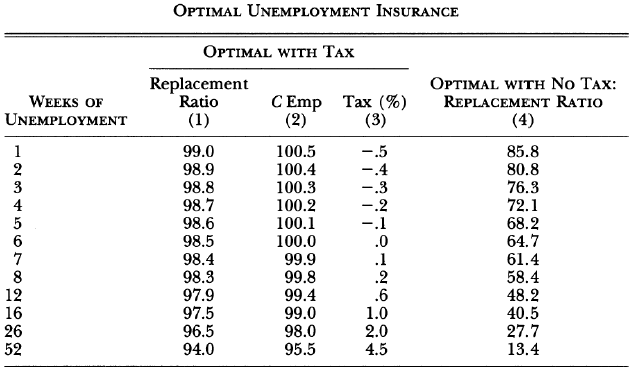
\includegraphics[width=8cm, height=6cm]{pic28}
    \end{center}
    Here the gains from using the employment tax can be large where agency's savings can increase by about 30%
\end{itemize}

\end{document}
